\begin{savequote}[75mm]
Nothing takes place in the world whose meaning is not that of some maximum or minimum.
\qauthor{--- Leonhard Euler ---}
\end{savequote}

\chapter{The graphical behaviour of functions}
\label{chap_behaviour}
\graphicspath{{figures/Behaviour/}}



Our study of limits led to continuous functions,  a certain class of functions that behave in a particularly nice way. Limits then gave us an even nicer class of functions, functions that are differentiable.

This chapter explores many of the ways we can take advantage of the information that continuous and differentiable functions  provide.

\section{Extreme values}\label{sec:extreme_values}

Given any quantity described by a function, we are often interested in the largest and/or smallest values that quantity attains. For instance, if a function describes the speed of an object, it seems reasonable to want to know the fastest/slowest the object traveled. If a function describes the value of a stock, we might want to know  the highest/lowest values the stock attained over the past year. We call such values \textbf{extreme values} (\textit{extrema}). 

\ifcalculus
\begin{definition}[Extreme values]\label{def:extreme_values}
Let $f$ be defined on an interval $I$ containing $c$.
	\begin{enumerate}[align=left]
	\item		$f(c)$ is the \textbf{minimum} (also, absolute minimum) of $f$ on $I$ if $f(c) \leq f(x)$ for all $x$ in $I$.
	\item		$f(c)$ is the \textbf{maximum} (also, absolute maximum) of $f$ on $I$ if $f(c) \geq f(x)$ for all $x$ in $I$.
	\end{enumerate}
	The maximum and minimum values are the extreme values, or extrema, of $f$ on $I$.\index{extrema!absolute}
\end{definition}
\fi


\ifanalysis
\begin{definition}[Extreme values]\label{def:extreme_values}
Let $f$ be defined on an interval $I$ containing $c$.
	\begin{enumerate}[align=left]
	\item		$f(c)$ is the \textbf{minimum} (also, absolute minimum) of $f$ on $I$ if 	$\forall\,x\in\,I:\,f(c) \leq f(x)$.
	\item		$f(c)$ is the \textbf{maximum} (also, absolute maximum) of $f$ on $I$ if $\forall\,x\in\,I:\,f(c) \geq f(x)$.
	\end{enumerate}
	The maximum and minimum values are the extreme values, or extrema, of $f$ on $I$.\index{extrema!absolute}
\end{definition}
\fi




\index{function ! (absolute) maximum}\index[aut]{functie ! (absoluut) maximum}
\index{function ! (absolute) minimum}\index[aut]{functie ! (absoluut) minimum}
\index{extreme values}\index[aut]{extreme waarden}
\index{absolute maximum}\index[aut]{absoluut maximum}
\index{absolute minimum}\index[aut]{absoluut minimum}
\index{maximum}\index[aut]{maximum}
\index{minimum}\index[aut]{minimum}
\index{extrema}\index[aut]{extrema}


We can also define relative minima and maxima, which may be understood as the smallest and largest $y$-value nearby, respectively. We can make this intuitive understanding more formal as follows. 


\begin{definition}[Relative minimum and relative maximum]\label{def:rel_ext}
Let $f$ be defined on an interval $I$ containing $c$. 
		\begin{enumerate}[align=left]
		\item	If there is a $\delta>0$ such that $f(c) \leq f(x)$ for all $x$ in $I$ where $|x-c|<\delta$, then $f(c)$ is a \textbf{relative minimum} (\textit{lokaal minimum}) of $f$. We also say that $f$ has a relative minimum at $(c,f(c))$. \index{minimum!relative/local}\index{extrema!relative}
		
		\item	If there is a $\delta>0$ such that $f(c) \geq f(x)$ for all $x$ in $I$ where $|x-c|<\delta$, then $f(c)$ is a \textbf{relative maximum} (\textit{lokaal maximum}) of $f$. We also say that $f$ has a relative maximum at $(c,f(c))$. \index{maximum!relative/local}\index{extrema!relative}
		\end{enumerate}
		
The relative maximum and minimum values comprise the \textbf{relative extrema} (\textit{lokaal extremum}) of $f$.
\end{definition}







\index{function ! (relative) maximum}\index[aut]{functie ! (relatief) maximum}
\index{function ! (relative) minimum}\index[aut]{functie ! (relatief) minimum}
\index{relative maximum}\index[aut]{relatief maximum}
\index{relative minimum}\index[aut]{relatief minimum}
\index{local maximum}\index[aut]{lokaal maximum}
\index{local minimum}\index[aut]{lokaal minimum}
\index{relative extrema}\index[aut]{relatieve extrema}

The function displayed in Figure~\ref{fig_behaviour_1a} has a maximum, but no minimum, as the interval over which the function is defined is open. In Figure~\ref{fig_behaviour_1b}, the function has a minimum, but no maximum; there is a discontinuity in the natural place for the maximum to occur. Finally, the function shown in Figure~\ref{fig_behaviour_1c} has both a maximum and a minimum; note that the function is continuous and the interval on which it is defined is closed. 

\begin{figure}[H]
\centering
%\raisebox{0.5cm}{
\subfigure[\label{fig_behaviour_1a}]{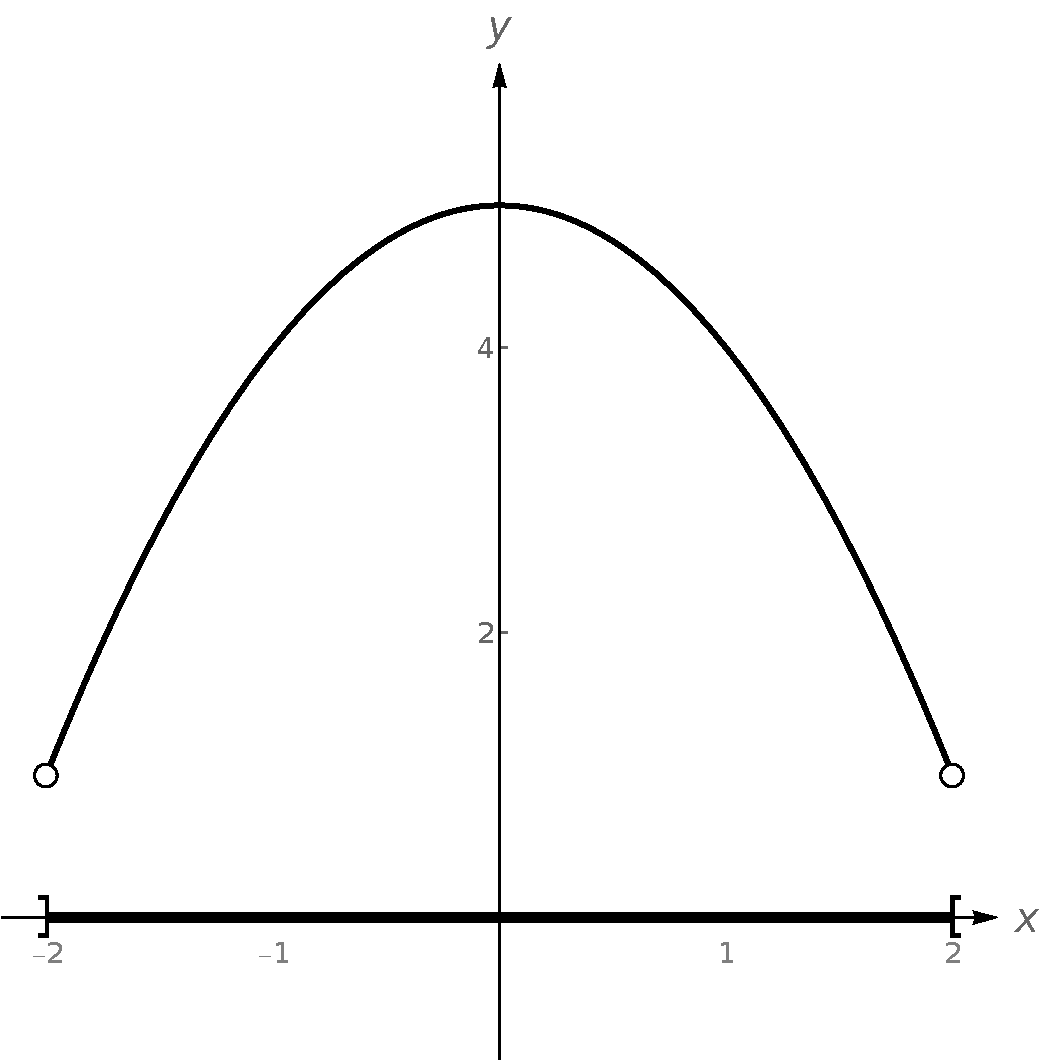
\includegraphics[width=0.35\textwidth]{fig_behaviour_1a}}
\qquad
\subfigure[\label{fig_behaviour_1b}]{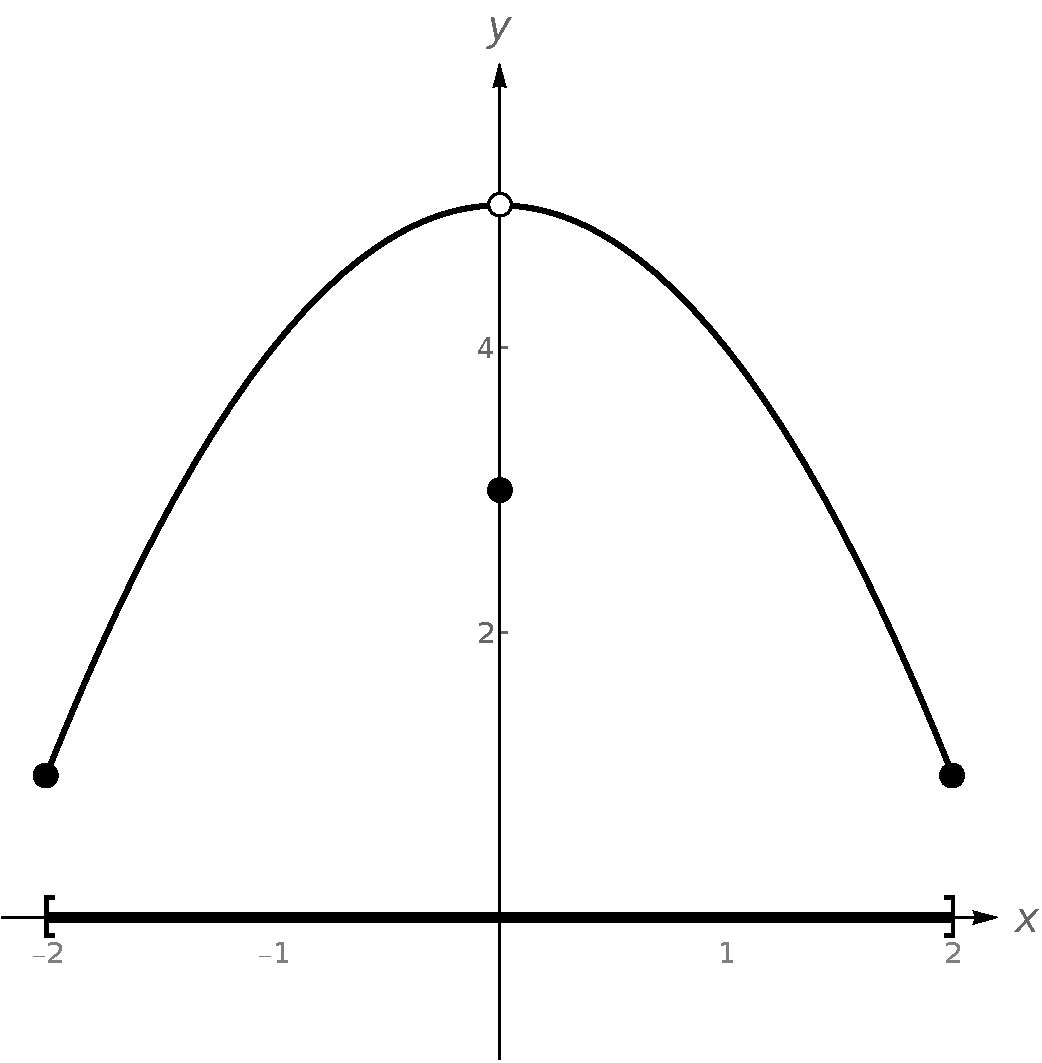
\includegraphics[width=0.35\textwidth]{fig_behaviour_1b} }
\qquad
\subfigure[\label{fig_behaviour_1c}]{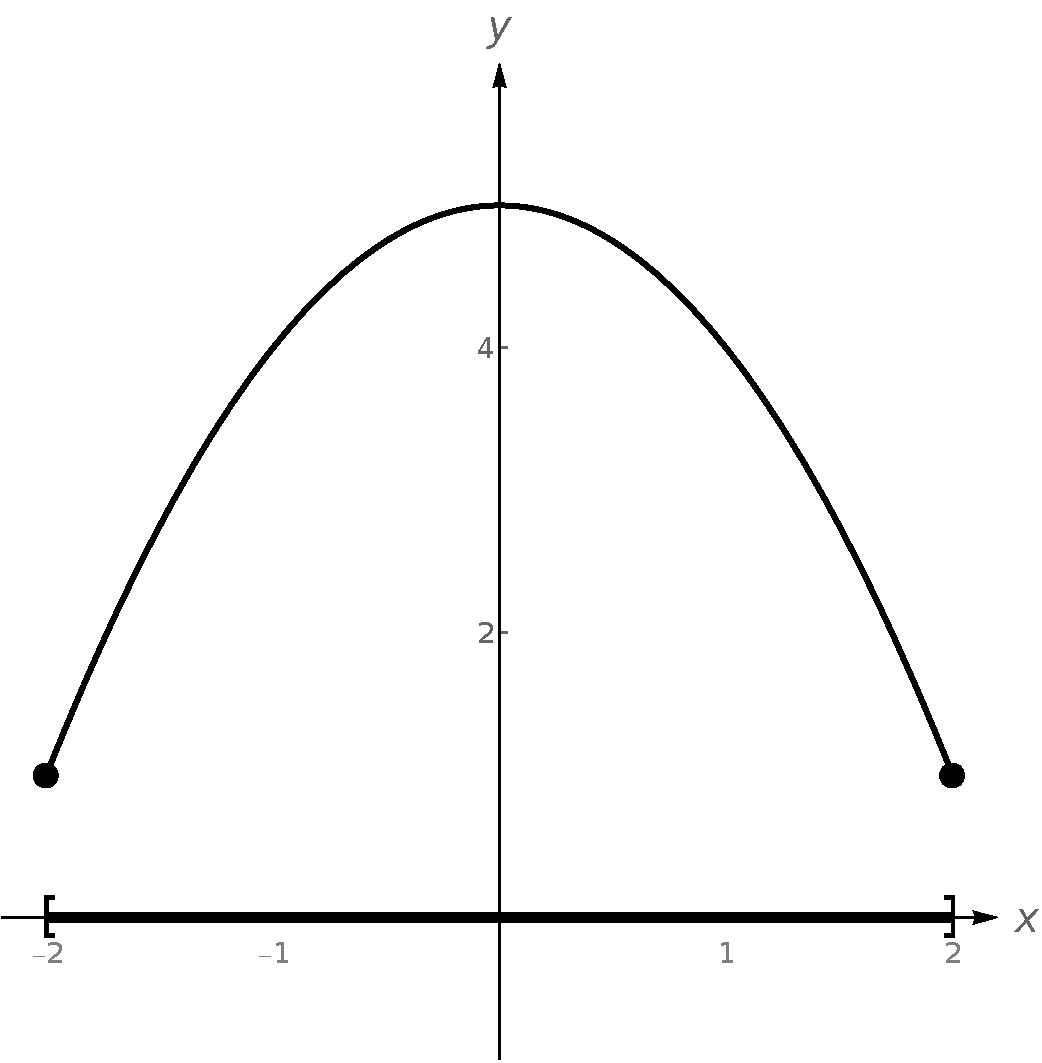
\includegraphics[width=0.35\textwidth]{fig_behaviour_1c} }
\caption{Graphs of functions with and without extreme values. }
\end{figure}

\pagebreak 
It is possible for discontinuous functions defined on an open interval to have both a maximum and minimum value, but we have just seen examples where they did not. On the other hand, continuous functions on a closed interval always have a maximum and minimum value. This is formalized in the following theorem. 

\begin{theorem}[The extreme value theorem]\label{thm:extreme_val}%
Let $f$ be a continuous function defined on a closed interval $I$. Then $f$ has both a maximum and minimum value on $I$.
\index{extreme value theorem}
\end{theorem}

\ifanalysis


\begin{proof}
The set $\{y\in\mathbb{R} : y = f(x), x \in [a,b]\}$ is a bounded set. Hence, its least upper bound exists by the least upper bound property of the real numbers. Let $M$ be this supremum, i.e.\ $M = sup(f(x))$ on $[a, b]$. If there is no point $x$ on $[a, b]$ so that $f(x) = M$, then $f(x) < M$ on $[a, b]$. Therefore, 
$$
\dfrac{1}{M-f(x)}
$$
 is continuous on $[a, b]$.

However, to every positive number $\epsilon$, there is always some $x$ in $[a, b]$ such that $M - f(x) < \epsilon$ because $M$ is the least upper bound. Hence, 
$$
\dfrac{1}{M - f(x)} > \dfrac{1}{\epsilon}\,,$$
which means that $1/(M - f(x))$ is not bounded. Since every continuous function on an interval $[a, b]$ is bounded (Theorem~\ref{thm_lim_fun_bound}), this contradicts the conclusion that $1/(M - f(x))$ was continuous on $[a, b]$. Therefore, there must be a point $x$ in $[a, b]$ such that $f(x) = M$. Consequently, the function $f$ attains its maximum value at some point in the interval $[a, b]$.

A similar reasoning is possible for what concerns the minimum. 
\end{proof}

\fi

This theorem states that $f$ has extreme values, but it does not offer any advice about how/where to find these values. The process can seem to be fairly easy, as the next example illustrates. After the example, we will draw on lessons learned to form a more general and powerful method for finding extreme values.



\begin{example}\label{ex_extval2}
Consider the functions
\begin{multicols}{2}
\begin{enumerate}
\item $f(x) = \dfrac{3x^4-4x^3-12x^2+5}{5}$, 
\item $g(x) = (x-1)^{2/3}+2$,
\end{enumerate}
\end{multicols}
as shown in Figure \ref{fig_behaviour_2a} and \ref{fig_behaviour_2b}, respectively. Approximate the relative extrema of these functions. At each of these points, evaluate the corresponding first derivative.

\begin{figure}[H]
\centering
%\raisebox{0.5cm}{
\subfigure[\label{fig_behaviour_2a}]{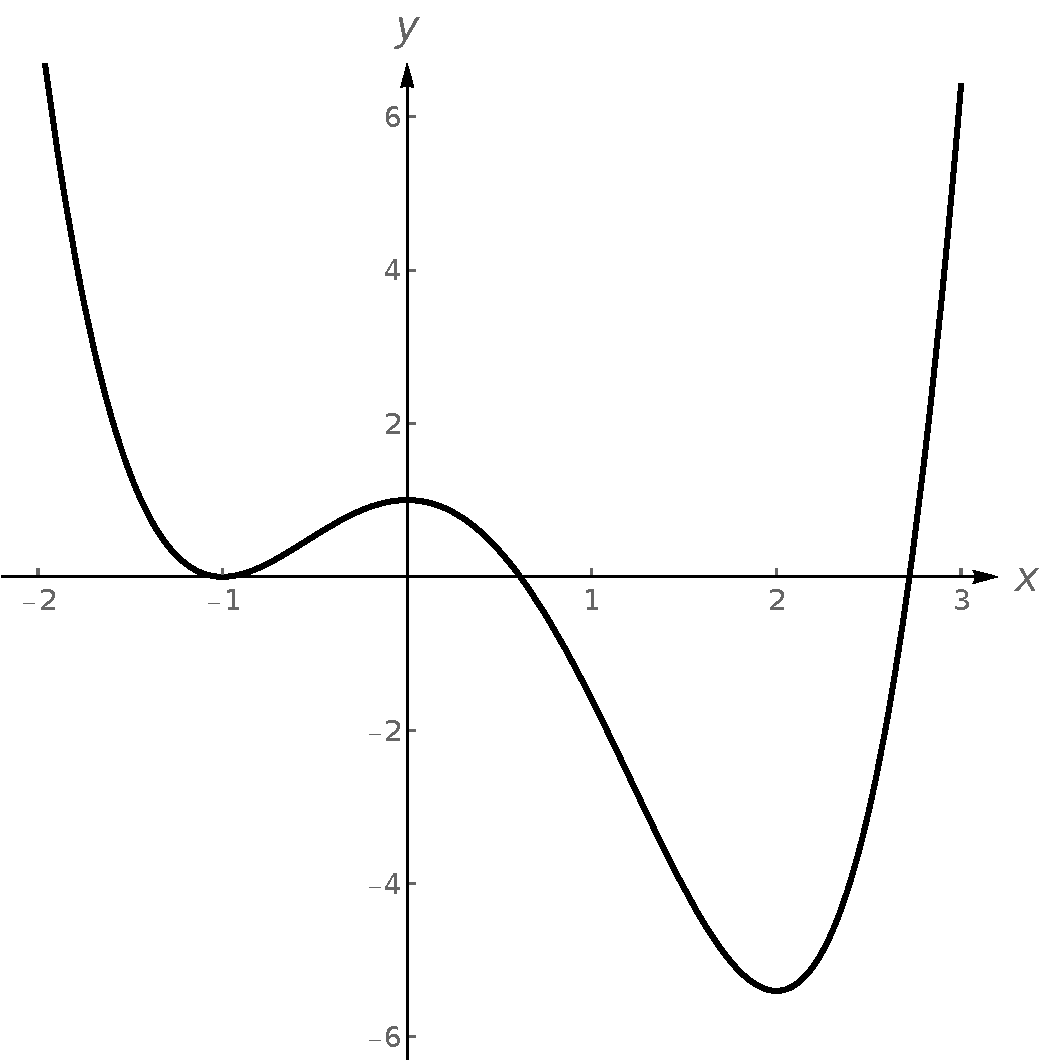
\includegraphics[width=0.4\textwidth]{fig_behaviour_2a}}
\qquad
\subfigure[\label{fig_behaviour_2b}]{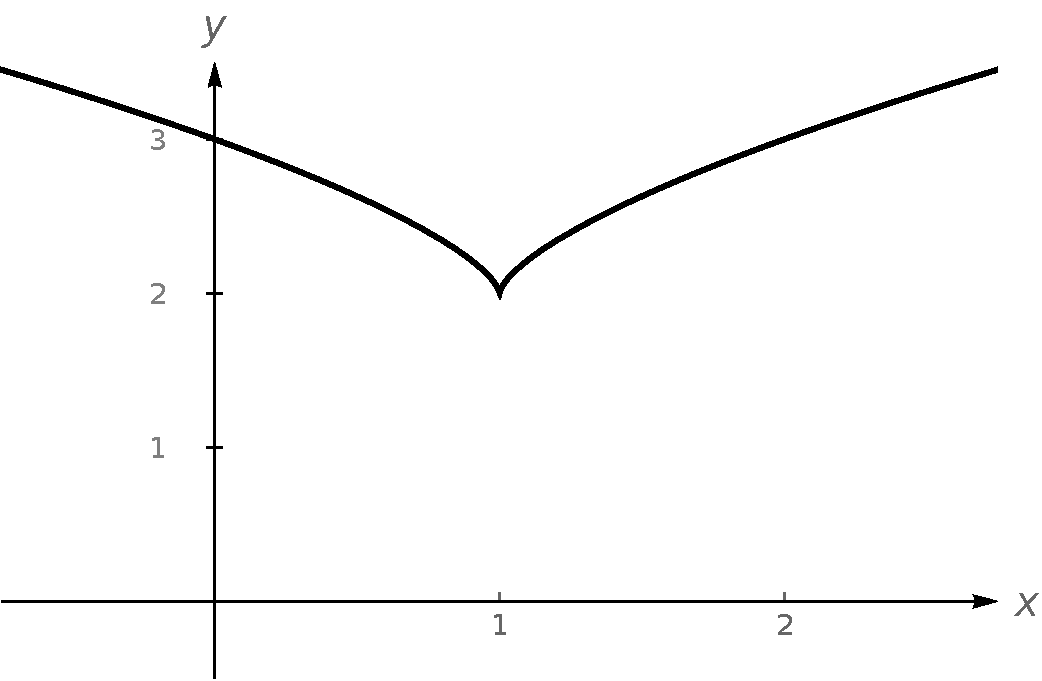
\includegraphics[width=0.4\textwidth]{fig_behaviour_2b}}
\caption{A graph of $f(x) = (3x^4-4x^3-12x^2+5)/5$ (a) and $g(x) = (x-1)^{2/3}+2$ (b). }
\end{figure}

\xhrulefill{gray}{2.5pt}Solution \xhrulefill{gray}{2.5pt}

We do not yet have the tools to exactly find the relative extrema, but the graphs do allow us to make reasonable approximations. 
\begin{enumerate}
\item It seems $f$ has relative minima at $x=-1$ and $x=2$, with values of $f(-1)=0$ and $f(2) = -5.4$. It also seems that $f$ has a relative maximum at the point $(0,1)$.  We approximate the relative minima to be $0$ and $-5.4$; we approximate the relative maximum to be $1$. It is straightforward to evaluate $\fp(x) =(12x^3-12x^2-24x)/5$ at $x=0, 1$ and $2$. In each case, $\fp(x) = 0$. 
\item Figure~\ref{fig_behaviour_2b} implies that $g$ does not have any relative maxima, but has a relative minimum at $(1,2)$. The graph suggests that not only is this point a relative minimum, $y=g(1)=2$ is the absolute minimum value of the function. We compute $g'(x) = 2/3(x-1)^{-1/3}$ note that when $x=1$, $g'$ is undefined.
\end{enumerate}
\end{example}

What can we learn from the previous two examples? We were able to visually approximate relative extrema, and at each such point, the derivative was either 0 or it was not defined. This observation holds for all functions, leading to a definition and a theorem.

\begin{definition}[Critical numbers and critical points]\label{def:criticalnum}%
Let $f$ be defined at $c$. The value $c$ is a \textbf{critical number} (or \textbf{critical value} (\textit{kritische waarde})) of $f$ if $\fp(c)=0$.\index{critical number}\index[aut]{kritieke waarde}\\
If $c$ is a critical number of $f$, then the point $(c,f(c))$ is a \textbf{critical point} (\textit{kritisch punt}) of $f$.\index[aut]{kritisch punt}\index{critical point}
\end{definition}


\begin{definition}[Singularities and singular points]\label{def:singularnum}%
Let $f$ be defined at $c$. The function has a \textbf{singularity} (\textit{singulariteit}) at $x=c$ if $f'(c)$ is not defined. The point $(c,f(c))$ is called the \textbf{singular point} (\textit{singulier punt}).\index{singular point}\index[aut]{singulier punt}
\end{definition}


\ifanalysis\pagebreak\fi
\begin{theorem}[Relative extrema and critical points]\label{thm:criticalpts}
Let a function $f$ be defined on an open interval $I$ containing $c$, and let $f$ have a relative extremum at the point $(c,f(c))$. Then $(c,f(c))$ is a critical or singular point of $f$.
\end{theorem}

In case the function $f$ is also differentiable on an open interval $I$ containing $c$, we restate Theorem~\ref{thm:criticalpts} as follows. 

\begin{theorem}[Fermat's theorem]\label{fermat}
Let a function $f$ be defined and differentiable on an open interval $I$ containing $c$, and let $f$ have a relative extremum at the point $(c,f(c))$. Then $f'(c)=0$.
\end{theorem}

\ifanalysis

\begin{proof}
We can prove Fermat's theorem by assuming that $x_{0}$ is a local maximum, and then prove that the derivative is 0 (a similar proof applies if $x_{0}$ is a local minimum). Then there exists a $\delta >0$ such that $]x_{0}-\delta ,x_{0}+\delta[\subset I$ and such that we have $f(x_{0})\geq f(x)$ for all $x$ with $ |x-x_{0}|<\delta$. Hence for any $h\in ]0,\delta[$ we notice that the following holds
$$
\displaystyle {\frac {f(x_{0}+h)-f(x_{0})}{h}}\leq 0\,.
$$

Since the limit of this ratio as $h$ gets close to 0 from above exists and is equal to $f'(x_{0})$  we conclude that $f'(x_{0})\leq 0$. On the other hand for $ h\in ]-\delta ,0[$ we notice that
$$
{\displaystyle {\frac {f(x_{0}+h)-f(x_{0})}{h}}\geq 0\,,}
$$
but again the limit as $h$ gets close to 0 from below exists and is equal to $f'(x_{0})$ so we also have $f'(x_{0})\geq 0$.

Hence we conclude that $f'(x_{0})=0$.
\end{proof}

\fi

Be careful to understand that Theorem~\ref{thm:criticalpts} states that relative extrema on open intervals occur at critical or singular points. It does not say that all such points produce relative extrema. For instance, consider the function $f(x) = x^3$. Since $\fp(x) = 3x^2$, it is straightforward to determine that $x=0$ is a critical number of $f$. However, $f$ has no relative extrema, as illustrated in Figure \ref{fig_behaviour_3}. 

\begin{figure}
	\begin{center}
			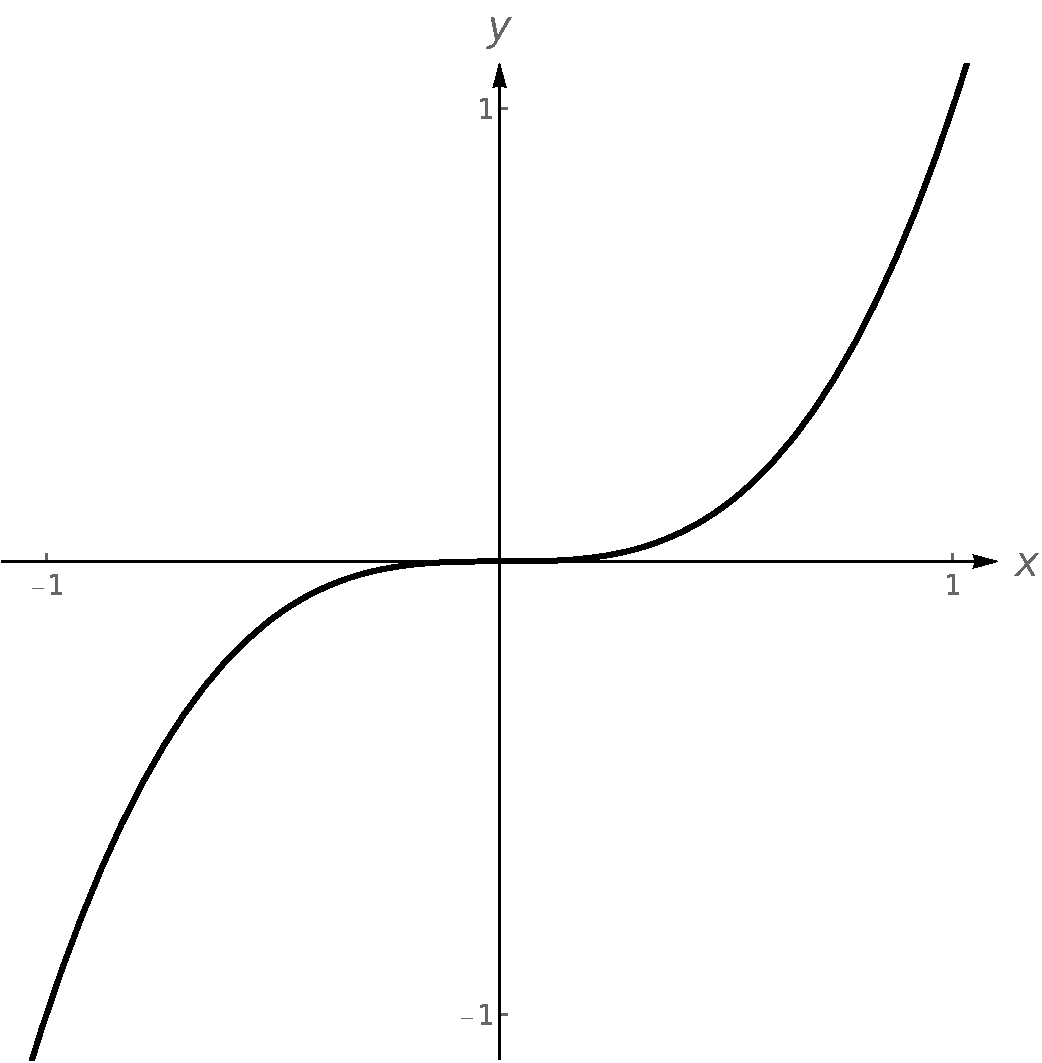
\includegraphics[width=0.35\textwidth]{fig_behaviour_3}
	\caption{A graph of $f(x)=x^3$ which has a critical value of $x=0$, but no relative extrema.}
	\label{fig_behaviour_3}
	\end{center}
\end{figure}


Theorem \ref{thm:extreme_val} states that a continuous function on a closed interval will have both an absolute maximum and an absolute minimum. Common sense tells us extrema occur either at the endpoints or somewhere in between. It is easy to check for extrema at endpoints, but there are infinitely many points to check that are in between. Our theory tells us we need only to check at the critical and singular points that are in between the endpoints. We combine these concepts to offer a strategy for finding extrema of a continuous function $f$ defined on a closed interval $[a,b]$. 
	\begin{enumerate}
	\item		Evaluate $f$ at the endpoints $a$ and $b$ of the interval.
	\item		Find the critical numbers and singularities of $f$ in $[a,b]$.
	\item		Evaluate $f$ at each critical number and singularity.
	\item		The absolute maximum of $f$ is the largest of these values, and the absolute minimum of $f$ is the least of these values.
	\end{enumerate}


We practice these ideas in the next examples.

\begin{example}\label{ex_extval6}
Find the extrema of the following functions
\begin{multicols}{2}
\begin{enumerate}
\item  $f(x) = \cos (x^2)$ on $[-2,2]$,
\item $g(x) = \sqrt{1-x^2}$,
\end{enumerate}
\end{multicols}
which are graphed in Figure~\ref{fig_behaviour_4a} and \ref{fig_behaviour_4b}, respectively.

\begin{figure}[H]
\centering
%\raisebox{0.5cm}{
\subfigure[\label{fig_behaviour_4a}]{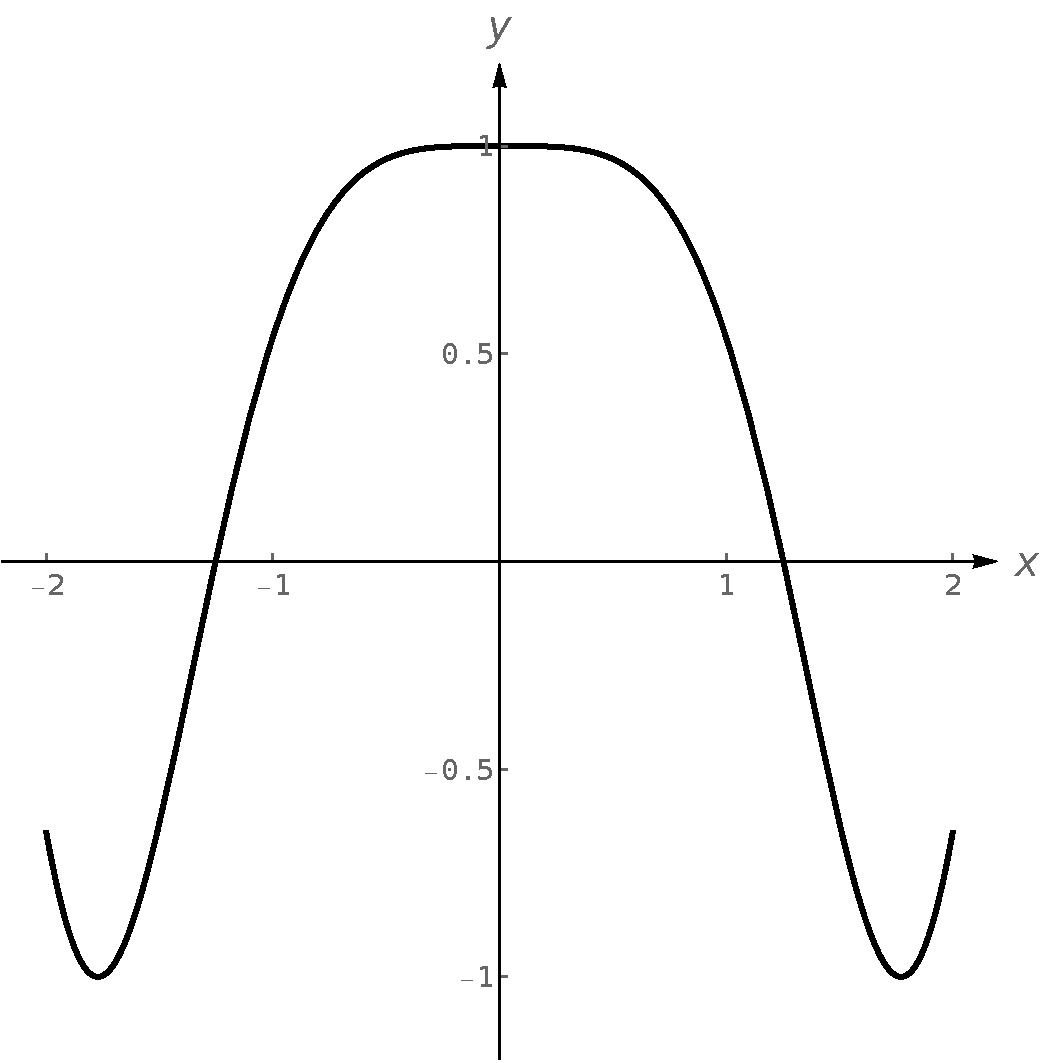
\includegraphics[width=0.35\textwidth]{fig_behaviour_4a}}
\qquad
\subfigure[\label{fig_behaviour_4b}]{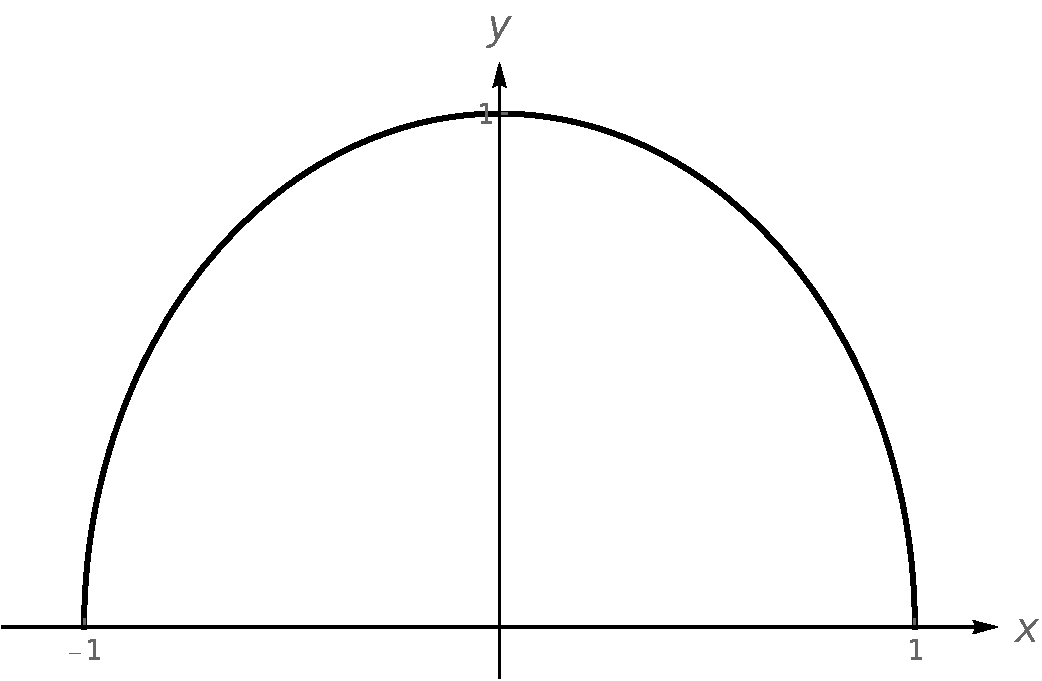
\includegraphics[width=0.35\textwidth]{fig_behaviour_4b}}
\caption{A graph of $f(x) = \cos (x^2)$ on $[-2,2]$ (a) and $g(x) = \sqrt{1-x^2}$ (b). }
\end{figure}

\xhrulefill{gray}{2.5pt}Solution \xhrulefill{gray}{2.5pt}

\begin{enumerate}
\item Evaluating $f$ at the endpoints of the interval gives: $f(-2) = f(2) = \cos (4) \approx -0.6536.$ We now find the critical values of $f$. Applying the chain rule, we find $\fp(x) = -2x\sin (x^2)$. Set $\fp(x) = 0$ and solve for $x$ to find the critical values of $f$. We do not have to bother about singularities because $f'$ is defined everywhere. 

We have $\fp(x) = 0$ when $x = 0$ and when $\sin (x^2) = 0$. In general, 
$$
\sin(t) = 0 \quad\Leftrightarrow\quad t = \ldots -2\pi, -\pi, 0, \pi, \ldots\,.
$$
Thus $\sin (x^2) = 0$ when $x^2 = 0, \pi, 2\pi, \ldots$ ($x^2$ is always positive so we ignore $-\pi$, etc.) So $\sin (x^2)=0$ when $x= 0, \pm \sqrt{\pi}, \pm\sqrt{2\pi},$ etc. The only values to fall in the given interval of $[-2,2]$ are $0$ and $\pm\sqrt{\pi}$, where $\sqrt{\pi} \approx 1.77$. We construct a table for the 5 important values: $x= 0, \pm 2, \pm\sqrt{\pi}$: 
\begin{center}
\begin{tabular}{c||ccccc} 
$x$ &$-2$&$-\sqrt{\pi}$&$0$&$\sqrt{\pi}$&$2$\\\hline
$f(x)$&$-0.65$ &$-1$&$1$&$-1$&$-0.65$
\end{tabular}
\end{center}


From this table it is clear that the maximum value of $f$ on $[-2,2]$ is 1 and occurs at $x=0$; the minimum value is $-1$ and occurs at $x=\pm\sqrt{\pi}$. The graph of $f$ in Figure~\ref{fig_behaviour_4a} confirms our results.
%\mfigure{.67}{A graph of $f(x)=\cos(x^2)$ on $[-2,2]$ as in Example \ref{ex_extval6}.}{fig:extval6}{figures/figextval6}

\item A closed interval is not given, so we find the extreme values of $g$ on its domain. $g$ is defined whenever $1-x^2\geq 0$; thus the domain of $g$ is $[-1,1]$. Evaluating $g$ at either endpoint returns 0. Using the chain rule, we find 
$$\ds g'(x) = \frac{-x}{\sqrt{1-x^2}}.$$
The critical points of $g$ are found when $g'(x) = 0$, and its singularities when $g'$ is undefined. It is straightforward to find that $g'(x) = 0$ when $x=0$, and $g'$ is undefined when $x=\pm 1$, the endpoints of the interval. We get the following table of important values:
\begin{center}
\begin{tabular}{c||ccc} 
$x$ &$-1$&$0$&$1$\\\hline
$g(x)$&$0$ &$1$&$0$
\end{tabular}
\end{center}

The maximum value is 1 and occurs at $x=0$. The minimum value is 0 and occurs at $x=\pm1$. 
\end{enumerate}
\end{example}

We can also find extrema of piecewise-defined functions as illustrated in the following example. 


\begin{example}\label{ex_extval5}
Find the maximum and minimum values of $f$ on $[-4,2]$, where $$f(x) = \left\{\begin{array}{cc} (x-1)^2, & x\leq 0 \\ x+1, & x>0. \end{array}\right. $$

\xhrulefill{gray}{2.5pt}Solution \xhrulefill{gray}{2.5pt}

Here $f$ is piecewise--defined, but we can still apply the same approach as before  since it is continuous on $[-4,2]$, i.e.\ $\ds\lim_{x\to0}f(x) =f(0)$. Evaluating $f$ at the endpoints gives: 
$$ f(-4) = 25 \quad \text{and} \quad f(2) = 3.$$

We now find the critical numbers and/or singularities of $f$. We have to define $\fp$ in a piecewise manner; it is 
$$\fp(x) =\left\{\begin{array}{cc} 2(x-1), & x < 0 \\ 1. & x>0. \end{array}\right. $$
 Note that while $f$ is defined for all of $[-4,2]$, $\fp$ is not, as the derivative of $f$ does not exist when $x=0$. From the left, the derivative approaches $-2$; from the right the derivative is 1. Thus $f$ has a singularity  at $x=0$.

We now set $\fp(x) = 0$. When $x >0$, $\fp(x)$ is never 0.  When $x<0$, $\fp(x)$ is also never 0, so we find no critical values from setting $\fp(x)=0$. So we have three important $x$ values to consider: $x= -4, 2$ and $0$. Evaluating $f$ at each gives, respectively, $25$, $3$ and $1$, shown in Table~\ref{fig_behaviour_5b}. Thus the absolute minimum of $f$ is 1, the absolute maximum of $f$ is $25$, confirmed by the graph of $f$ in Figure~\ref{fig_behaviour_5a}.

\begin{figure}[H]
  \centering
  \subfigure[\label{fig_behaviour_5a}]{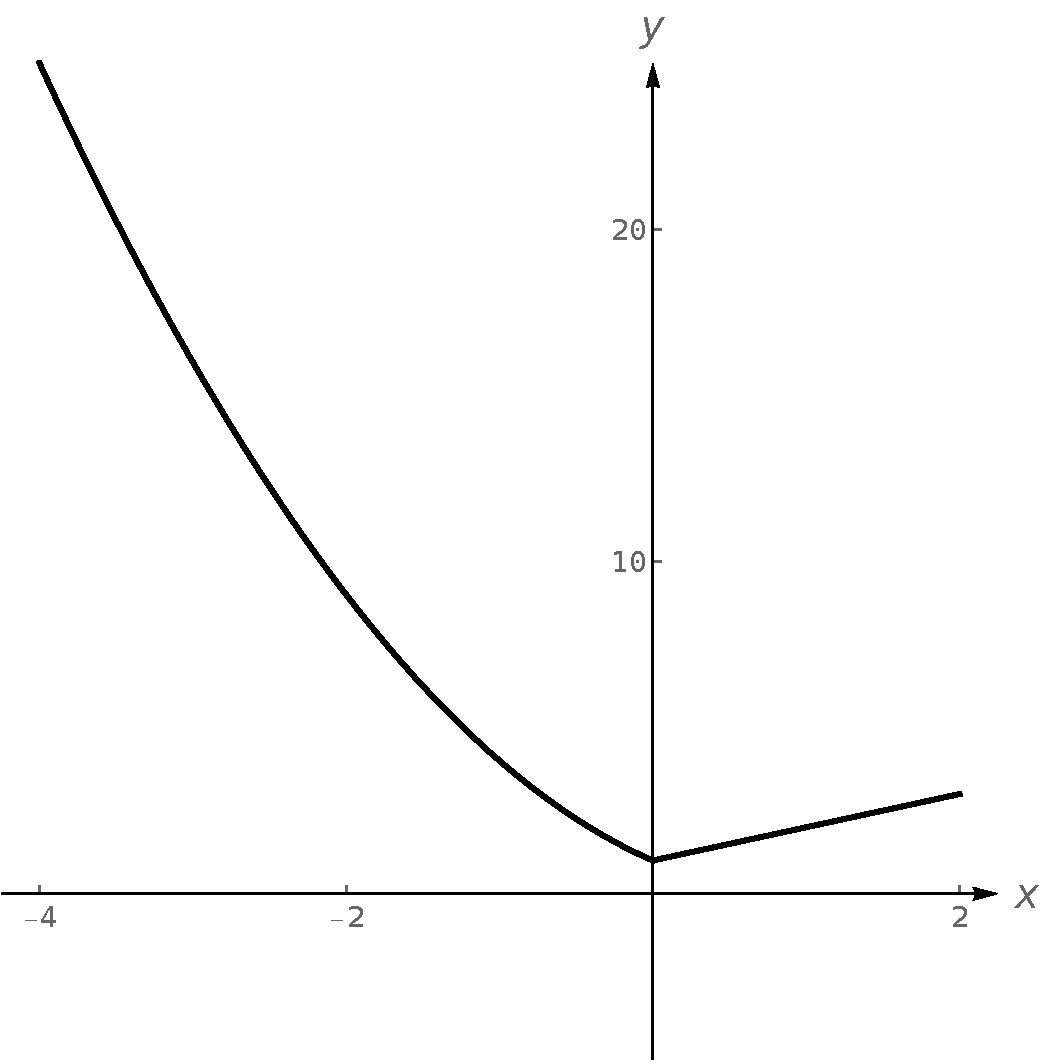
\includegraphics[width=0.35\textwidth]{fig_behaviour_5a}}%
  \qquad
  \subfigure[\label{fig_behaviour_5b}]{
\begin{tabular}[b]{c|c} $x$ & $f(x)$ \\ \hline\hline \rule{0pt}{10pt} $-4$ & 25 \\ 0 & 1 \\ 2 & 3\end{tabular}
  }
\caption{A graph of $f(x)$ on $[-4,2]$ as in Example \ref{ex_extval5} (a) and finding the extrema of $f$ (b).}
\end{figure}

\end{example}


In the next section, we further our study of the information we can glean from nice functions with the mean value theorem. On a closed interval, we can find the average rate of change of a function. We will see that differentiable functions always have a point at which their instantaneous rate of change is same as the average rate of change. This is surprisingly useful, as we will see.


\section{The mean value theorem}\label{sec:mvt}
\subsection{Introduction}
We motivate this section with the following question: Suppose you leave your house and drive to your friend's house in a city 100 kilometres away, completing the trip in two hours.  At any point during the trip do you necessarily have to be going 50 kilomteres per hour?

In answering this question, it is clear that the average speed for the entire trip is 50 km/hr, but the question is whether or not your instantaneous speed is ever exactly 50 km/hr.  The answer, under some very reasonable assumptions, is yes.

Let us now see why this situation is in a calculus text by translating it into mathematical symbols.\\

First assume that the function $y = f(t)$ gives the distance (in kilometres) travelled from your home at time $t$ (in hours) where $0\le t\le 2$.  In particular, this gives $f(0)=0$ and $f(2)=100$.  The slope of the secant line connecting the starting and ending points $(0,f(0))$ and $(2,f(2))$ is therefore 
$$
\frac{\Delta f}{\Delta t} = \frac{f(2)-f(0)}{2-0} = \frac{100-0}{2} = 50 \, \text{km/hr}.
$$

The slope at any point on the graph itself is given by the derivative $\fp(t)$.  So, since the answer to the question above is yes, this means that at some time during the trip, the derivative takes on the value of 50 km/hr.  Symbolically, 
$$
\fp(c) = \frac{f(2)-f(0)}{2-0} = 50
$$
for some time $0\le c \le 2.$\\

How about more generally?  Given any function $y=f(x)$ and a range $a\le x\le b$ does the value of the derivative at some point between $a$ and $b$ have to match the slope of the secant line connecting the points $(a,f(a))$ and $(b,f(b))$?  Or equivalently, does the equation 
$$\fp(c) = \frac{f(b)-f(a)}{b-a}$$
have to hold for some $a < c < b$?


Consider, for instance, the functions $$f_1(x)=\frac{1}{x^2}\quad \text{and} \quad f_2(x) = |x|$$ with $a=-1$ and $b=1$ as shown in Figure~\ref{fig_behaviour_6} (a) and (b), respectively.  Both functions have a value of 1 at $a$ and $b$.  Therefore the slope of the secant line connecting the end points is $0$ in each case.  But if you look at the plots of each, you can see that there are no points on either graph where the tangent lines have slope zero. Therefore we have found that there is no $c$ in $[-1,1]$ such that $$\fp(c) = \frac{f(1)-f(-1)}{1-(-1)} = 0.$$

\begin{figure}[H]
\centering
%\raisebox{0.5cm}{
\subfigure[\label{fig_behaviour_6a}]{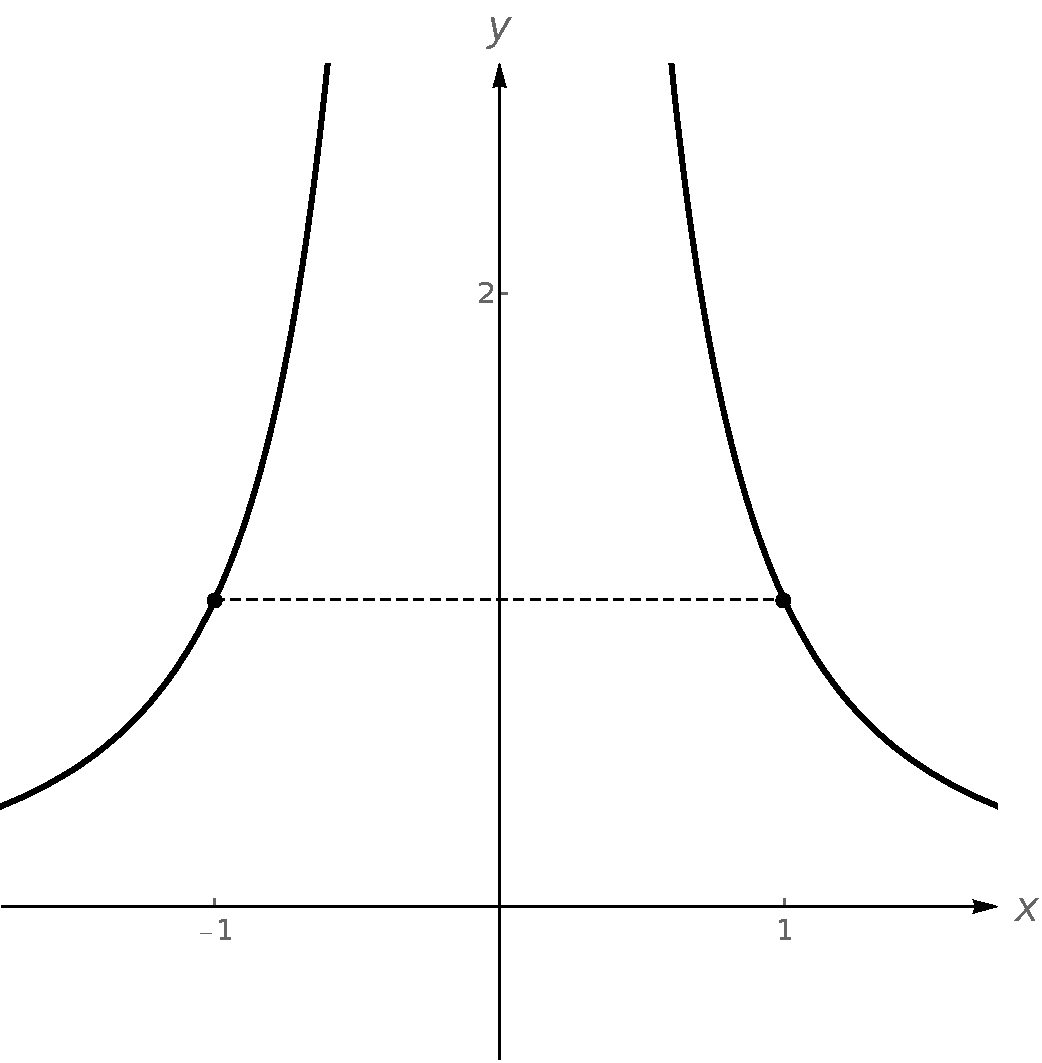
\includegraphics[width=0.3\textwidth]{fig_behaviour_6a}}
\qquad
\subfigure[\label{fig_behaviour_6b}]{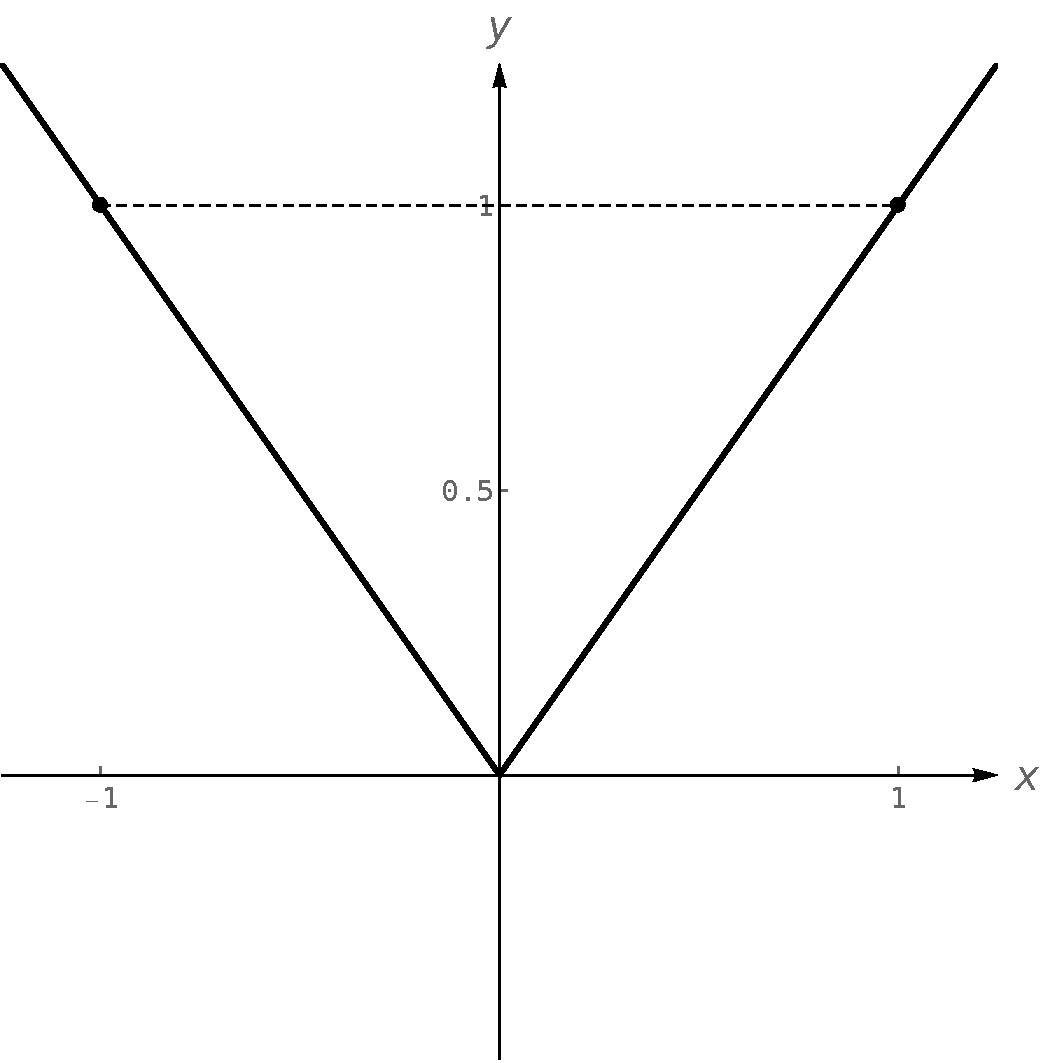
\includegraphics[width=0.3\textwidth]{fig_behaviour_6b}}
\caption{A graph of $f_1(x) = 1/x^2$ (a) and $f_2(x) = |x|$ (b). }
\label{fig_behaviour_6}
\end{figure}

\subsection{The theorems}
So what went wrong?  It may not be surprising to find that the discontinuity of $f_1$ and the corner of $f_2$ play a role.  If our functions had been continuous and differentiable, would we have been able to find that special value $c$? This is our motivation for the following theorem, which is sometimes also referred to as Lagrange's theorem. 

\begin{theorem}[The mean value theorem of differentiation]\label{thm:mvt}
Let $y=f(x)$ be a continuous function on the closed interval $[a,b]$ and differentiable on the open interval $]a,b[$. There exists a value $c$, with $a < c < b$, such that \index{mean value theorem}\index[aut]{middelwaardestelling}
$$
\fp(c) = \frac{f(b)-f(a)}{b-a}.
$$
That is, there is a value $c$ in $]a,b[$ where the instantaneous rate of change of $f$ at $c$ is equal to the average rate of change of $f$ on $[a,b]$.
\end{theorem}

Note that the reasons that the functions graphed in Figures~\ref{fig_behaviour_6a} and \ref{fig_behaviour_6b} fail are indeed that $f_1$ has a discontinuity on the interval $[-1,1]$ and $f_2$ is not differentiable at the origin.\\

\ifanalysis We will give a proof of the mean value theorem below. To do so, we use a fact, called Rolle's theorem, stated here.\fi
\ifcalculus The proof of the mean value theorem relies on the Rolle's theorem, which we also include to increase the understanding of the mean value theorem. \fi

\begin{theorem}[Rolle's theorem]\label{thm:rolles}
Let $f$ be continuous on $[a,b]$ and differentiable on $]a,b[$, where $f(a) = f(b)$. There is some $c$ in $]a,b[$ such that $\fp(c) = 0.$\index{Rolle's Theorem}\index[aut]{Rolle ! stelling van}
\end{theorem}

Consider Figure \ref{fig_behaviour_7} where the graph of a function $f$ is given, where $f(a) = f(b)$. It should make intuitive sense that if $f$ is differentiable (and hence, continuous) that there would be a value $c$ in $]a,b[$ where $\fp(c)=0$; that is, there would be a relative maximum or minimum of $f$ in $]a,b[$. Rolle's theorem guarantees at least one; there may be more. 

\begin{figure}[h]
	\begin{center}
			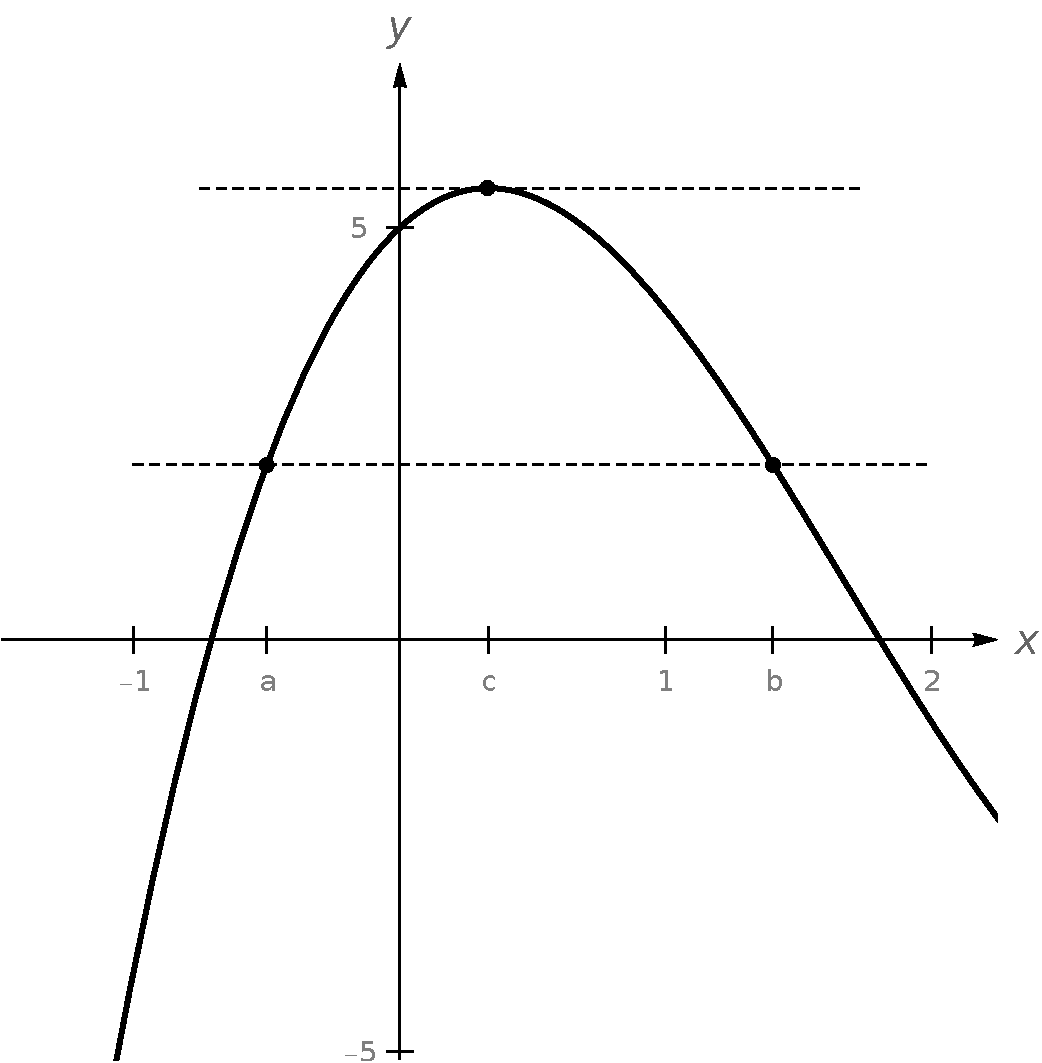
\includegraphics[width=0.5\textwidth]{fig_behaviour_7}
	\caption{A graph of $f(x) = x^3-5x^2+3x+5$, where $f(a) = f(b)$. Note the existence of $c$, where $a<c<b$, where $\fp(c)=0$.}
	\label{fig_behaviour_7}
	\end{center}
\end{figure}


Rolle's theorem is really just a special case of the mean value theorem. If $f(a) = f(b)$, then the average rate of change on $]a,b[$ is $0$, and the theorem guarantees some $c$ where $\fp(c)=0$. \ifanalysis We will prove Rolle's theorem, then use it to prove the mean value theorem.


\noindent\textbf{Proof of Rolle's theorem}
\begin{proof}
Let $f$ be differentiable on $]a,b[$ where $f(a)=f(b)$. We consider two cases. 

\noindent\textbf{Case 1:} Consider the case when $f$ is constant on $[a,b]$; that is, $f(x) = f(a) = f(b)$ for all $x$ in $[a,b]$. Then $\fp(x) = 0$ for all $x$ in $[a,b]$, showing there is at least one value $c$ in $]a,b[$ where $\fp(c)=0$.

\noindent\textbf{Case 2:} Now assume that $f$ is not constant on $[a,b]$. The extreme value theorem guarantees that $f$ has a maximal and minimal value on $[a,b]$, found either at the endpoints or at a critical value in $]a,b[$. Since $f(a)=f(b)$ and $f$ is not constant, it is clear that the maximum and minimum cannot both be found at the endpoints. Assume, without loss of generality, that the maximum of $f$ is not found at the endpoints. Therefore there is a $c$ in $]a,b[$ such that $f(c)$ is the maximum value of $f$. By Theorem~\ref{thm:criticalpts}, $c$ must be a critical number of $f$; since $f$ is differentiable, we have that $\fp(c) = 0$, completing the proof of the theorem. \\
\end{proof}
We can now prove the mean value theorem.\\

\noindent\textbf{Proof of the mean value theorem}
\begin{proof}
Define the function $$g(x) = f(x) - \frac{f(b)-f(a)}{b-a}x.$$  We know $g$ is differentiable on $]a,b[$ and  continuous on $[a,b]$ since $f$ is. We can show $g(a)=g(b)$, though it is actually easier to show $g(b)-g(a)=0$, which suffices. We can then apply Rolle's theorem to guarantee the existence of $c$ in %\in 
$]a,b[$ such that $g'(c) = 0$.  But note that $$0= g'(c) = \fp(c) - \frac{f(b)-f(a)}{b-a}$$ hence $$\fp(c) = \frac{f(b)-f(a)}{b-a},$$ which is what we sought to prove.
\end{proof}

\fi

	\checkoddpage
\marginpar{\ifoddpage\hspace*{-1.5cm}\else\hspace*{0.25cm}\fi
\includegraphics[width=0.075\textwidth]{youtube}\\
\ifoddpage\hspace*{-1.75cm}\else\hspace*{0.1cm}\fi
\qrcode[height=1.75cm]{https://youtu.be/6hri9k_2R8o}
%\includegraphics[width=0.1\textwidth]{mvt}
}

Going back to the very beginning of the section, we see that the only assumption we would need about our distance function $f(t)$ is that it be continuous and differentiable for $t$ from 0 to 2 hours (both reasonable assumptions).  By the mean value theorem, we are guaranteed a time during the trip where our instantaneous speed is 50 km/hr. This fact is used in practice. Some law enforcement agencies monitor traffic speeds while in aircraft. They do not measure speed with radar, but rather by timing individual cars as they pass over lines painted on the highway whose distances apart are known. The officer is able to measure the average speed of a car between the painted lines; if that average speed is greater than the posted speed limit, the officer is assured that the driver exceeded the speed limit at some time.

Finally, note that the man value theorem is an \textbf{existence theorem} (\textit{existentiestelling}). It states that a special value $c$ exists, but it does not give any indication about how to find it. It turns out that when we need the mean value theorem, existence is all we need.

\begin{example}\label{ex_mvt2}

Consider $f(x) = x^3+5x+5$ on $[-3,3]$. Find $c$ in $[-3,3]$ that satisfies the mean value theorem.

\xhrulefill{gray}{2.5pt}Solution \xhrulefill{gray}{2.5pt}

The average rate of change of $f$ on $[-3,3]$ is:
		$$\frac{f(3)-f(-3)}{3-(-3)} = \frac{84}{6} = 14.$$
		
We want to find $c$ such that $\fp(c) = 14$. We find $\fp(x) = 3x^2+5$. We set this equal to 14 and solve for $x$. 
\[ \begin{array}{rrcl}
		& \fp(x) &=& 14 \\
		\Rightarrow \quad & 3x^2 +5 &= & 14\\
		\Leftrightarrow & x^2  &=& 3\\
		\Leftrightarrow & x &=& \pm \sqrt{3} \approx \pm 1.732
\end{array}\] 
	
We have found 2 values $c$ in $[-3,3]$ where the instantaneous rate of change is equal to the average rate of change; the mean value theorem guaranteed at least one. In Figure \ref{fig_behaviour_8}, $f$ is graphed with a dashed line representing the average rate of change; the lines tangent to $f$ at $x=\pm \sqrt{3}$ are also given. Note how these lines are parallel (i.e., have the same slope) with the dashed line.
\begin{figure}[H]
	\begin{center}
			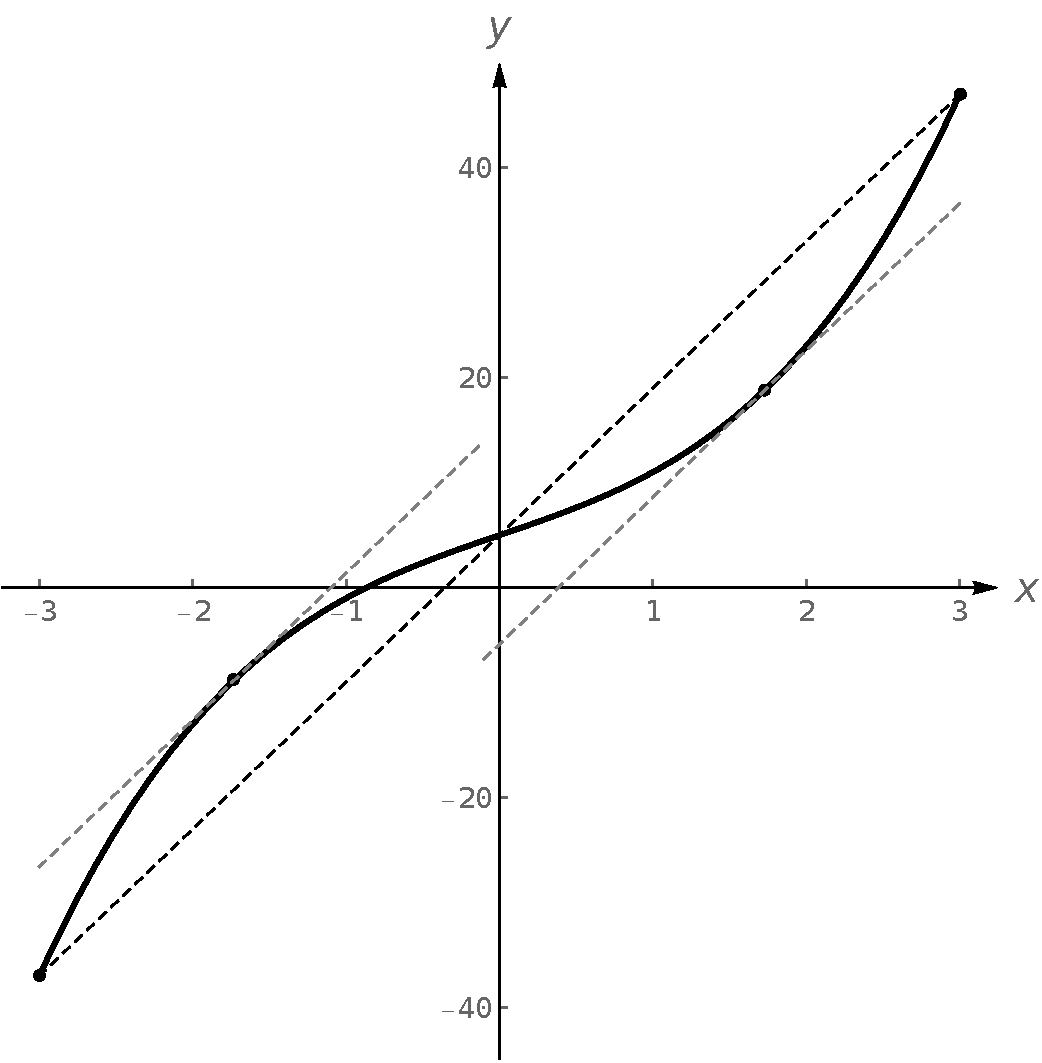
\includegraphics[width=0.4\textwidth]{fig_behaviour_8}
	\caption{Demonstrating the mean value theorem in Example \ref{ex_mvt2}.}
	\label{fig_behaviour_8}
	\end{center}
\end{figure}

\end{example}

While the mean value theorem has practical use, such as the speed monitoring application mentioned before, it is mostly used to advance other theory. We will use it in the next section to relate  the shape of a graph to its derivative.


\section{Increasing and decreasing functions}\label{sec:incr_decr}

Our study of nice functions $f$ in this chapter has so far focused on individual points: points where $f$ is maximal/minimal, points where $\fp(x) = 0$ or $\fp$ does not exist, and points $c$ where $\fp(c)$ is the average rate of change of $f$ on some interval. 

In this section we begin to study how functions behave between special points; we begin studying in more detail the shape of their graphs by recalling the following definition from Chapter~\ref{chap_functions}.

\ifcalculus
\begin{definition}[Increasing and decreasing functions]\label{def:incr_decr}
Let $f$ be a function defined on an interval $I$.\index{function ! increasing}\index{function ! decreasing}%\index{increasing function!strictly}\index{decreasing function!strictly}
\begin{enumerate}
\item		$f$ is \textbf{increasing} (\textit{stijgend}) on $I$ if for every $a<b$ in $I$, $f(a) \leq f(b)$.
\item		$f$ is \textbf{decreasing} (\textit{dalend}) on $I$ if for every $a<b$ in $I$, $f(a) \geq f(b)$.
\item		$f$ is \textbf{constant} (\textit{constant}) on $I$ if for every $a<b$ in $I$, $f(a) = f(b)$.
\end{enumerate}
\end{definition}
\fi
\ifanalysis
\begin{definition}[Increasing and decreasing functions]\label{def:incr_decr}
Let $f$ be a function defined on an interval $I$.\index{function ! increasing}\index{function ! decreasing}%\index{increasing function!strictly}\index{decreasing function!strictly}
\begin{enumerate}
\item		$f$ is \textbf{increasing} (\textit{stijgend}) on $I$ if $\left(\forall a,b\in\,I\mid\,a<b\Rightarrow f(a)\leq f(b)\right)$.
\item		$f$ is \textbf{decreasing} (\textit{dalend}) on $I$ if $\left(\forall a,b\in\,I\mid\,a<b\Rightarrow f(a)\geq f(b)\right)$.
\item $f$ is \textbf{constant} (\textit{constant}) on $I$ if $\left(\forall a,b\in\,I\mid\,a<b\Rightarrow f(a)= f(b)\right)$.
\end{enumerate}
\end{definition}
\fi
\index[aut]{functie ! dalend}\index[aut]{functie ! stijgend}

Informally, a function is increasing if as $x$ gets larger (i.e., looking left to right) $f(x)$ gets larger, i.e.\ it does not decrease. Also recall that if the order $\leq$ in the definition of an increasing function is replaced by $<$,  we say that $f$ is \textbf{strictly increasing} (\textit{strikt stijgend}) on the interval $I$, and likewise for a \textbf{strictly decreasing} (\textit{strikt dalend}) function.

Our interest lies in finding intervals in the domain of $f$ on which $f$ is either increasing or decreasing. Such information should seem useful. For instance, if $f$ describes the speed of an object, we might want to know when the speed was increasing or decreasing (i.e., when the object was accelerating vs. decelerating). If $f$ describes the population of a city, we should be interested in when the population is growing or declining.

To find such intervals, we again consider secant lines. Let $f$ be a strictly increasing, differentiable function on an open interval $I$, such as the one shown in Figure \ref{fig_behaviour_9}, and let $a<b$ be given in $I$. The secant line on the graph of $f$ from $x=a$ to $x=b$ is drawn; it has a slope of $(f(b)-f(a))/(b-a)$. But note:
$$
\frac{f(b)-f(a)}{b-a} \qquad\Rightarrow\qquad \frac{\text{numerator }>0}{\text{denominator } >0} \qquad\Rightarrow\quad \parbox{70pt}{\centering slope of the secant line $>0$}
\quad\Rightarrow\quad \parbox{70pt}{\centering Average rate of change of $f$ on $[a,b]$ is $>0$.}$$


\begin{figure}[h]
	\begin{center}
			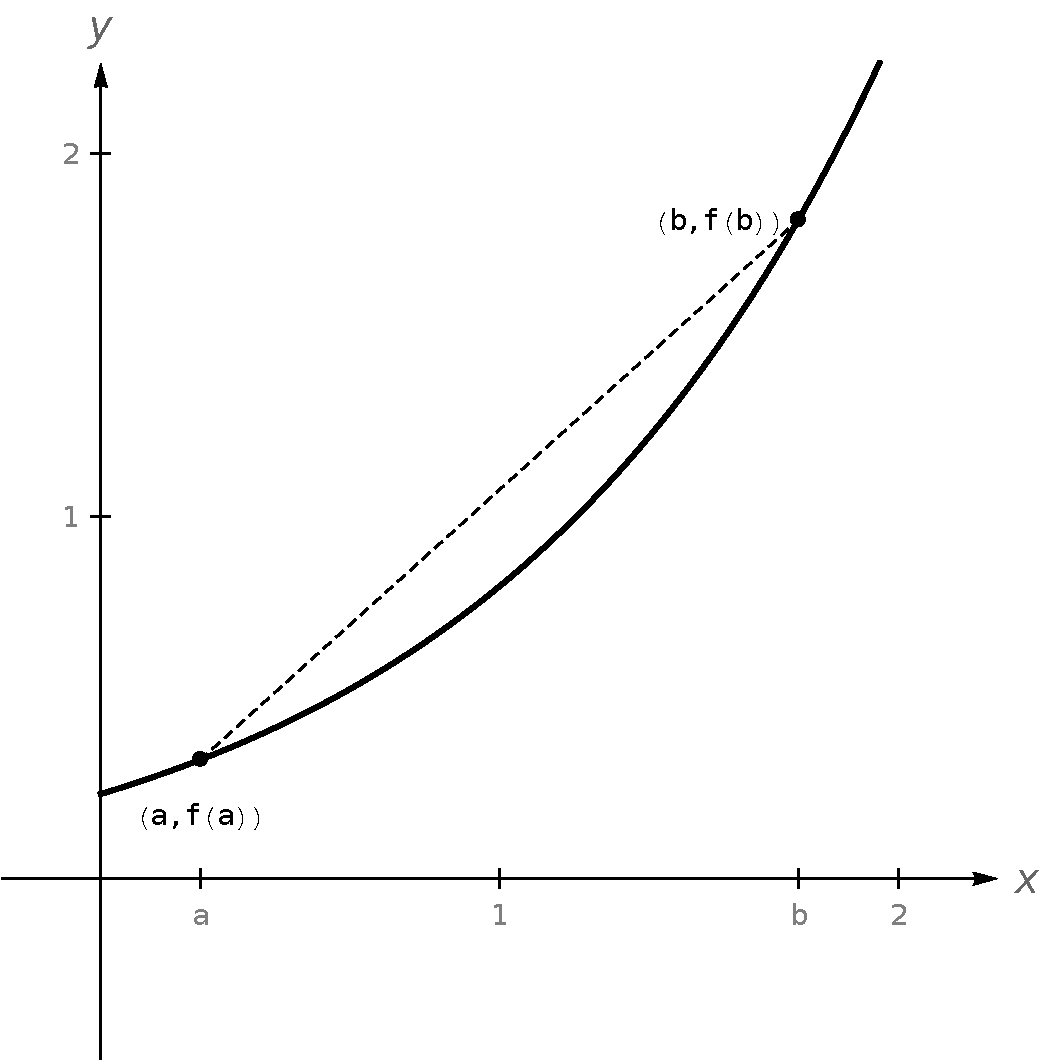
\includegraphics[width=0.35\textwidth]{fig_behaviour_9}
	\caption{Examining the secant line of an increasing function.}
	\label{fig_behaviour_9}
	\end{center}
\end{figure}


We have shown mathematically what may have already been obvious: when $f$ is strictly increasing, its secant lines will have a positive slope. Now recall the mean value theorem guarantees that there is a number $c$, where $a<c<b$, such that $$\fp(c) = \frac{f(b)-f(a)}{b-a}>0.$$ By considering all such secant lines in $I$, we strongly imply that $\fp(x) > 0$ on $I$. A similar statement can be made for strictly decreasing functions.

Our above logic can be summarized as If $f$ is strictly  increasing, then $\fp$ is probably  positive. Theorem~\ref{thm:incr_decr} turns this around by stating If $\fp$ is positive, then $f$ is strictly increasing. This leads us to a method for finding when functions are strictly increasing and decreasing.

\begin{theorem}[Test for increasing/decreasing functions]\label{thm:incr_decr}%
Let $f$ be a continuous function on $[a,b]$ and differentiable on $\left.\right]a,b\left[\right.$.
\begin{enumerate}
\item		If $\fp(c) > 0$ for all $c$ in $]a,b[$, then $f$ is strictly increasing on $[a,b]$.
\item		If $\fp(c) <0$ for all $c$ in $]a,b[$, then $f$ is strictly decreasing on $[a,b]$.
\item		If $\fp(c) =0$ for all $c$ in $]a,b[$, then $f$ is constant on $[a,b]$.
\end{enumerate}
\end{theorem}


\ifanalysis

\begin{proof}
The proof of this fact uses the mean value theorem we introduced in the preceding section. 

Let us start with the first statement in the theorem, namely that if $\fp(c) > 0$ for all $c$ in $]a,b[$, then $f$ is strictly increasing on $[a,b]$.

Let $x_1$ and $x_2$ be in $[a,b]$ and suppose that $x_1<x_2$. Now, using the mean value theorem on $[x_1,x_2]$ means there is a number $c$ such that $x_1<c<x_2$ and,
$$
f\left( {{x_2}} \right) - f\left( {{x_1}} \right) = f'\left( c \right)\left( {{x_2} - {x_1}} \right)\,.
$$
Because $x_1<c<x_2$ we know that $c$ must also be in $[a,b]$ and so we know that $f'(c)>0$. We also know that $x_2-x_1>0$. So, this means that we have,
$$
f\left( {{x_2}} \right) - f\left( {{x_1}} \right) > 0\,.
$$
Rewriting this gives
$$
f\left( {{x_2}} \right) > f\left( {{x_1}} \right)\,,
$$
and so, by definition, since $x_1$ and $x_2$ were two arbitrary numbers in $[a,b]$, $f(x)$ must be strictly increasing on this interval.

This proof for the two other statements in Theorem~\ref{thm:incr_decr} is nearly identical. 
%http://tutorial.math.lamar.edu/Classes/CalcI/DerivativeAppsProofs.aspx
\end{proof}

\fi

Let $f$ be differentiable on an interval $I$ and let $a$ and $b$ be in $I$ where $\fp(a)>0$ and $\fp(b)<0$. If $\fp$ is continuous on $[a,b]$, it follows from the intermediate value theorem (Theorem~\ref{thm:IVT}) that there must be some value $c$ between $a$ and $b$ where $\fp(c) = 0$. It turns out that this is still true even if $\fp$ is not continuous on $[a,b]$. This leads us to the following method for finding intervals on which a function is strictly increasing or decreasing.


Let $f$ be a differentiable function on an interval $I$. To find intervals on which $f$ is increasing and decreasing:
\begin{enumerate}
\item	Find the critical values and singular points of $f$. That is, find all $c$ in $I$ where $\fp(c) = 0$ or $\fp$ is not defined.
\item		Use the critical values and singular points to divide $I$ into subintervals.
\item		Pick any point $p$ in each subinterval, and find the sign of $\fp(p)$. 
		\begin{enumerate}
		\item		If $\fp(p)>0$, then $f$ is strictly increasing on that subinterval.
		\item		If $\fp(p)<0$, then $f$ is strictly decreasing on that subinterval.
		\end{enumerate}
\end{enumerate}


Note that parts 1 \& 2 of Theorem~\ref{thm:incr_decr} also hold if $\fp(c) = 0$ for a finite number of values of $c$ in $I$.  Hence, acknowledging the difference between increasing and strictly increasing functions, we may say that
\begin{enumerate}
\item if $f'(p)\geq0$, then $f$ is increasing.
\item if $f'(p)\leq0$, then $f$ is decreasing.
\end{enumerate}



We demonstrate using this process in the following example.

\begin{example}\label{ex_incr1}
Let $f(x) = x^3+x^2-x+1$. Find intervals on which $f$ is strictly increasing or decreasing.

\xhrulefill{gray}{2.5pt}Solution \xhrulefill{gray}{2.5pt}

Following the method outlined above, we first find the critical values of $f$. Hence, we have \\ $\fp(x) = 3x^2+2x-1 = (3x-1)(x+1)$, so $\fp(x) = 0$ when $x=-1$ and when $x=1/3$. $\fp$ is never undefined.

Since an interval was not specified for us to consider, we consider the entire domain of $f$ which is $\mathbb{R}$. We thus break the whole real line into three intervals based on the two critical values we just found: $\left.\right]-\infty,-1\left[\right.$, $\left.\right]-1,1/3\left[\right.$ and $\left.\right]1/3,+\infty\left[\right.$.


We now pick a value $p$ in each interval and find the sign of $\fp(p)$. All we care about is the sign, so we do not actually have to fully compute $\fp(p)$; pick nice values that make this simple.
\begin{description}
\item \textbf{Interval 1: $\left.\right]-\infty,-1\left[\right.$}

We (arbitrarily) pick $p=-2$. We can compute $\fp(-2)$ directly: $$\fp(-2) = 3(-2)^2+2(-2)-1=7>0.$$ We conclude that $f$ is increasing on $\left.\right]-\infty,-1\left[\right.$.

Note we can arrive at the same conclusion without computation. For instance, we could choose $p=-100$. The first term in $\fp(-100)$, i.e., $3(-100)^2$ is clearly positive and very large. The other terms are small in comparison, so we know $\fp(-100)>0$. All we need is the sign.

\item \textbf{Interval 2: $\left.\right]-1,1/3\left[\right.$}

We pick $p=0$ since that value seems easy to deal with. $\fp(0) = -1<0$. We conclude $f$ is decreasing on $\left.\right]-1,1/3\left[\right.$.

\item\textbf{Interval 3: $\left.\right]1/3,+\infty\left[\right.$}

Pick an arbitrarily large value for $p>1/3$ and note that $\fp(p) =3p^2+2p-1 >0$. We conclude that $f$ is increasing on $\left.\right]1/3,\infty\left[\right.$.

\end{description}
In summary, we find: 
	\begin{center}
			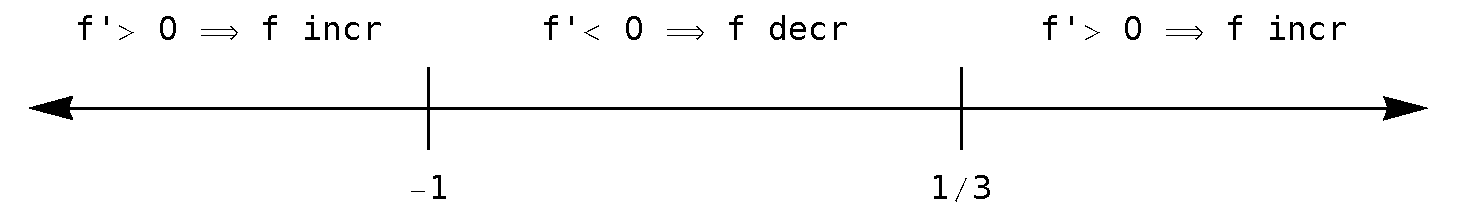
\includegraphics[width=0.65\textwidth]{fig_behaviour_10}
	\end{center}
	
We can verify our calculations by considering Figure \ref{fig_behaviour_11}, where $f$ is graphed. The graph also presents $\fp$; note how $\fp>0$ when $f$ is strictly increasing and $\fp<0$ when $f$ is strictly decreasing.

\begin{figure}[H]
	\begin{center}
			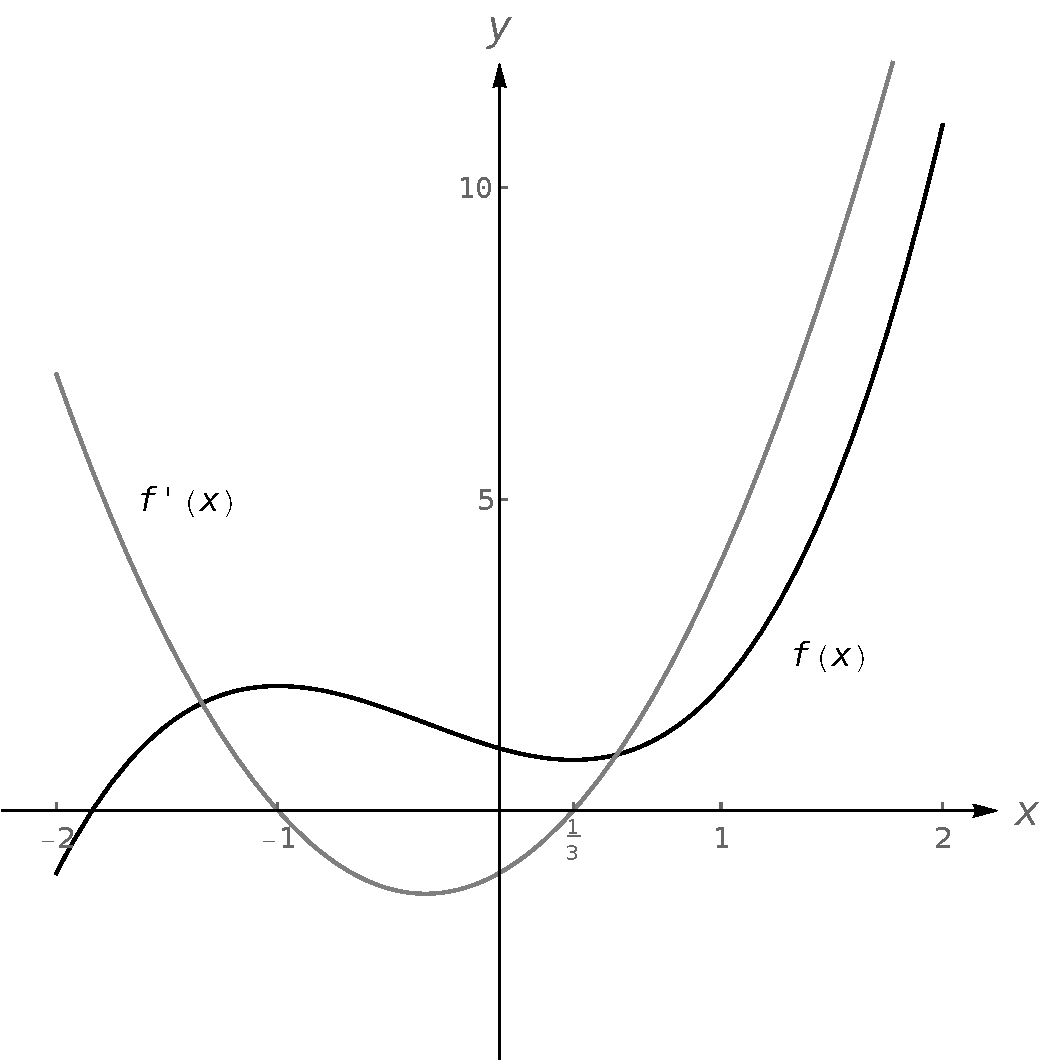
\includegraphics[width=0.45\textwidth]{fig_behaviour_11}
	\caption{A graph of $f(x)$ (black)  and $f'(x)$ (gray) in Example \ref{ex_incr1}, showing where $f$ is increasing and decreasing.}
	\label{fig_behaviour_11}
	\end{center}
\end{figure}

\end{example}

In Section~\ref{sec:extreme_values} we learned the definition of relative maxima and minima and found that they occur at critical points. We are now learning from Example~\ref{ex_incr1} that functions can switch from increasing to decreasing (and vice--versa) at critical points. This new understanding of increasing and decreasing creates a great method of determining whether a critical  point corresponds to a maximum, minimum, or neither. Imagine a function increasing until a critical point at $x=c$, after which it decreases. A quick sketch helps confirm that $f(c)$ must be a relative maximum. A similar statement can be made for relative minimums. We formalize this concept in a theorem.

%\small
%\setboxwidth{100pt}
\begin{theorem}[First derivative test]\label{thm:first_der}
Let $f$ be differentiable on an interval $I$ and let $c$ be a critical number in $I$.\index{First Derivative Test}
\begin{enumerate}
\item		If the sign of \fp\ switches from positive to negative at $c$, then $f(c)$ is a relative maximum of $f$.
\item		If the sign of \fp\ switches from negative to positive at $c$, then $f(c)$ is a relative minimum of $f$.
%\item		If the sign of \fp\ does not change at $c$, then $f(c)$ is not a relative extrema of $f$.
\item		If \fp\ is positive (or, negative) before and after $c$, then $f(c)$ is not a relative extremum of $f$.
\end{enumerate}
\end{theorem}

\ifanalysis

\begin{proof}
We only prove the first statement in this theorem because the proofs of the other statements are similar. 

In this case, we have that $f'$ is positive on $]a,c[$ and negative on $]c,b[$. Let $x$ be an arbitrary point in $]a,c[$. Since $f$ is differentiable on $]a,c[$ and continuous at $c$, it is continuous on $[x,c]$ and differentiable on $]x,c[$. So, by the mean value theorem, there is a $x_0$ in $]x,c[$ such that
$$
\dfrac{f(c)-f(x)}{c-x}=f'(x_0)\,.
$$
Because $x_0$ is in $]x,c[$ too, it holds that $f'(x_0)>0$. And since we also have that $c-x>0$, it immediately follows that $f(c)-f(x)>0$, or $f(x)<f(c)$. A similar argument shows that for all $x$ in $]c,b[$, we have that $f(x)<f(c)$. Let $h=\min(c-a,b-c)$. Consequently, for all $x$ in $]c-h,c[\cup]c,c+h[$ it holds that $f(x)<f(c)$. Hence, for all $x$ in $]c-h,c+h[$, we have that $f(x)\leq f(c)$, which implies that $f$ has a local maximum at $c$.
\end{proof}

% http://www.phengkimving.com/calc_of_one_real_var/05_app_of_the_der_part_1/05_03_the_first_der_test.htm

\fi

\begin{example}
\label{ex_incr2}
Find the intervals on which $f$ is increasing and decreasing, and determine the relative extrema of $f$,  where 
$$f(x) = \frac{x^2+3}{x-1}.$$

\xhrulefill{gray}{2.5pt}Solution \xhrulefill{gray}{2.5pt}

We start by noting the domain of $f$: $]-\infty,1[ \, \cup \, ]1,+\infty[$. Since the domain of $f$ in this example is the union of two intervals, we apply Theorem~\ref{thm:first_der} to both intervals of the domain of $f$. 

Since $f$ is not defined at $x=1$, the increasing/decreasing nature of $f$ could switch at this value. At this point $f$ manifests a singularity, so we should keep track of it. 

Using the quotient rule, we find
$$\fp(x) = \frac{x^2-2x-3}{(x-1)^2}.$$
We can now find the critical values and possible further singular points of $f$; we want to know when $\fp(x)=0$ and when $\fp$ is not defined. That latter is straightforward: when the denominator of $\fp(x)$ is 0, $\fp$ is undefined. That occurs when $x=1$, which we have already recognized as an important value.


$\fp(x)=0$ when the numerator of $\fp(x)$ is 0. That occurs when $x^2-2x-3 = (x-3)(x+1) = 0$; i.e., when $x=-1,3$. 

We have found that $f$ has two critical numbers, $x=-1,3$, and at $x=1$ something important might also happen. These three numbers divide the real number line into 4 subintervals: 
$$]-\infty,-1[, \quad ]-1, 1[, \quad ]1,3[ \quad \text{and} \quad ]3,+\infty[.$$ Pick a number $p$ from each subinterval and test the sign of \fp\ at $p$ to determine whether $f$ is increasing or decreasing on that interval. Again, we do well to avoid complicated computations; notice that the denominator of $\fp$ is always positive so we can ignore it during our work.

\begin{description}
\item \textbf{Interval 1:} $]-\infty,-1[$

Choosing a very small number (i.e., a negative number with a large magnitude) $p$ returns $p^2-2p-3$ in the numerator of $\fp$; that will be positive. Hence $f$ is increasing on $]-\infty,-1[$.

\item \textbf{Interval 2:} $]-1,1[$

Choosing 0 seems simple: $\fp(0)=-3<0$. We conclude $f$ is decreasing on $]-1,1[$.

\item\textbf{Interval 3:} $]1,3[$

Choosing 2 seems simple: $\fp(2) = -3<0$. Again, $f$ is decreasing.

\item \textbf{Interval 4:} $]3,+\infty[$

Choosing an very large number $p$ from this subinterval will give a positive numerator and (of course) a positive denominator. So $f$ is increasing on $]3,+\infty[$.

\end{description}


In summary, $f$ is increasing on the intervals $]-\infty,-1[$ and $]3,+\infty[$ and is decreasing on the intervals $]-1,1[$ and $]1,3[$. Since at $x=-1$, the sign of \fp\ switched from positive to negative, Theorem \ref{thm:first_der} states that $f(-1)$ is a relative maximum of $f$. At $x=3$, the sign of \fp\ switched from negative to positive, meaning $f(3)$ is a relative minimum. At $x=1$, $f$ is not defined, so there is no relative extremum at $x=1$.


This is summarized in the number line below. Also, Figure \ref{fig_behaviour_13} shows a graph of $f$, confirming our calculations. This figure also shows $\fp$, again demonstrating that $f$ is increasing when $\fp>0$ and decreasing when $\fp<0$.

	\begin{center}
			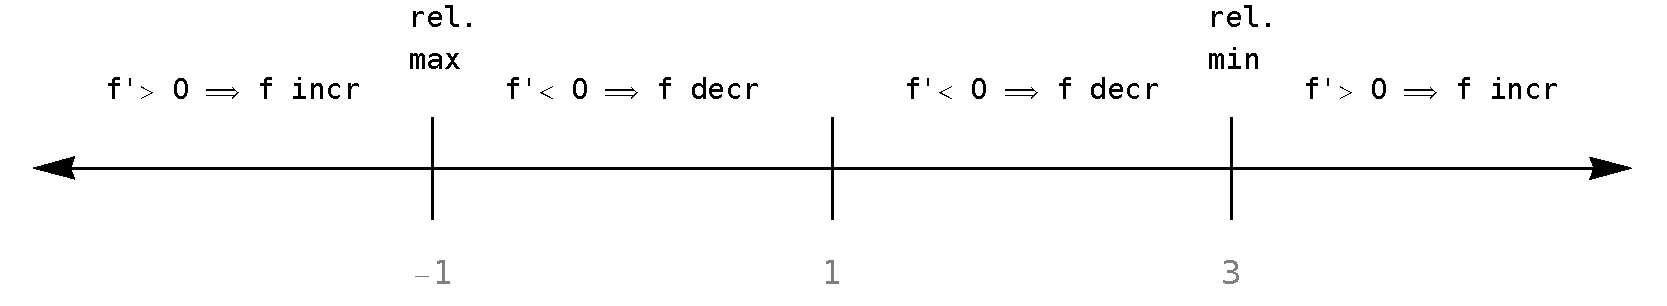
\includegraphics[width=0.9\textwidth]{fig_behaviour_12}
	\end{center}

\begin{figure}[H]
	\begin{center}
			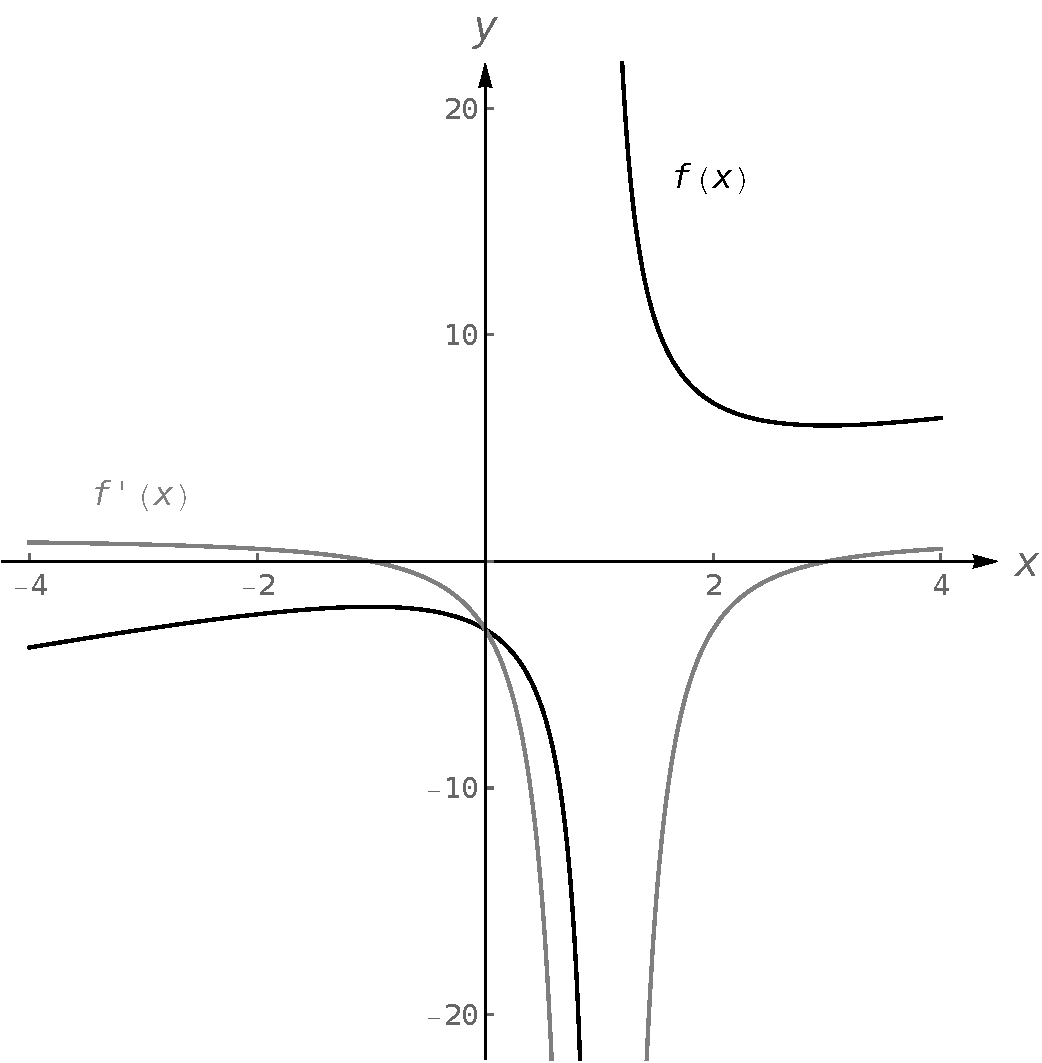
\includegraphics[width=0.5\textwidth]{fig_behaviour_13}
	\caption{A graph of $f(x)$  and $f'(x)$ in Example \ref{ex_incr2}, showing where $f$ is increasing and decreasing.}
	\label{fig_behaviour_13}
	\end{center}
\end{figure}

\end{example}

We examine one example. 
\begin{example}\label{ex_incr3}
Find the intervals on which $f(x) = x^{8/3}-4x^{2/3}$ is increasing and decreasing and identify the relative extrema.

\xhrulefill{gray}{2.5pt}Solution \xhrulefill{gray}{2.5pt}

We start with taking a derivative. Since we know we want to solve $\fp(x) = 0$, we will do some algebra after taking the derivative.

\allowdisplaybreaks
\begin{align*}
f(x) &= x^{\frac{8}{3}}-4x^{\frac{2}{3}} \\
\Rightarrow\quad\fp(x) &= \frac{8}{3} x^{\frac{5}{3}} - \frac{8}{3}x^{-\frac{1}{3}}\\[0.2cm]
	&= \frac{8}{3}x^{-\frac{1}{3}}\left(x^{\frac{6}{3}}-1\right)\\[0.2cm]
	&=\frac{8}{3}x^{-\frac{1}{3}}(x^2-1)\\[0.2cm]
	&=\frac{8}{3}x^{-\frac{1}{3}}(x-1)(x+1).
\end{align*}

This derivation of $\fp$ shows that $\fp(x) = 0$ when $x=\pm 1$ and \fp\ is not defined when $x=0$. Thus we have 2 critical values and one singular point, breaking the number line into 4 subintervals.  

	

\begin{description}
\item \textbf{Interval 1: $\left.\right]-\infty,-1\left[\right.$}

We choose $p=-2$; we can easily verify that $\fp(-2)<0$. So $f$ is decreasing on $\left.\right]-\infty,-1\left[\right.$.

\item \textbf{Interval 2:  $\left.\right]-1,0\left[\right.$}

 Choose $p=-1/2$. We can once more find the sign of $\fp(p)$ without computing an actual value. We have $\fp(p) = (8/3)p^{-1/3}(p-1)(p+1)$; find the sign of each of the three terms. 
		$$\fp(p) = \frac{8}{3} \cdot \underbrace{p^{-\frac13}}_{<0}\cdot \underbrace{(p-1)}_{<0}\underbrace{(p+1)}_{>0}.$$
		Consequently,  $f$ is increasing on $\left.\right]-1,0\left[\right.$.
		
\item\textbf{Interval 3: $\left.\right]0,1\left[\right.$}

We do a similar sign analysis as before, using $p$ in $\left.\right]0,1\left[\right.$.
		$$\fp(p) = \frac{8}{3} \cdot \underbrace{p^{-\frac13}}_{>0}\cdot \underbrace{(p-1)}_{<0}\underbrace{(p+1)}_{>0}.$$
		We have 2 positive factors and one negative factor; $\fp(p)<0$ and so $f$ is decreasing on $\left.\right]0,1\left[\right.$.
		
\item \textbf{Interval 4:  $\left.\right]1,+\infty\left[\right.$} Similar work to that done for the other three intervals shows that $\fp(x)>0$ on $\left.\right]1,+\infty\left[\right.$, so $f$ is increasing on this interval.
\end{description}
Finally, we have:
\begin{center}
			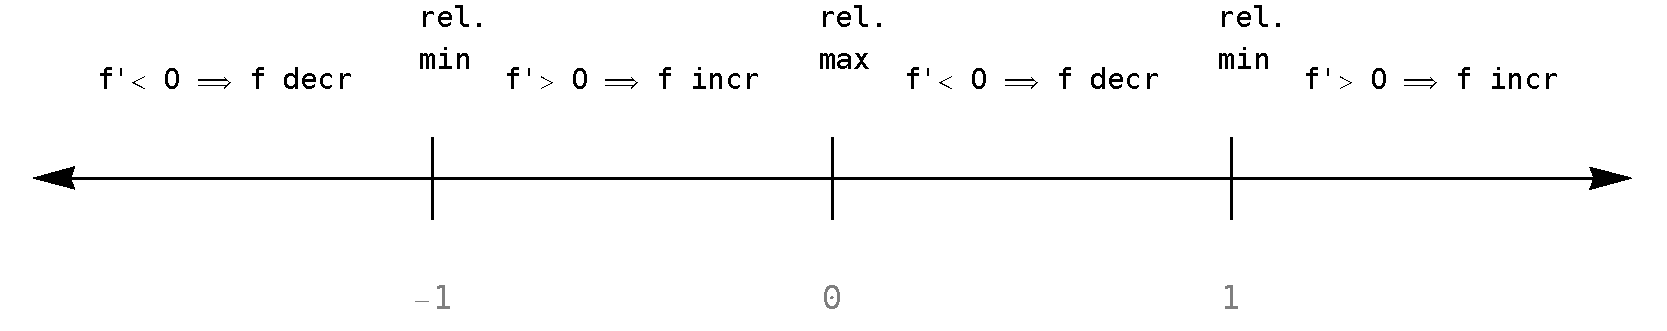
\includegraphics[width=0.9\textwidth]{fig_behaviour_14}
	\end{center}
	
Consequently, we conclude by stating that $f$ is increasing on the intervals $\left.\right]-1,0\left[\right.$ and $\left.\right]1,+\infty\left[\right.$ and decreasing on the intervals $\left.\right]-\infty,-1\left[\right.$ and $\left.\right]0,1\left[\right.$. The sign of \fp\ changes from negative to positive around $x=-1$ and $x=1$, meaning by Theorem \ref{thm:first_der} that $f(-1)$ and $f(1)$ are relative minima of $f$. As the sign of \fp\ changes from positive to negative at $x=0$, we have a relative maximum at $f(0)$. Figure \ref{fig_behaviour_15} shows a graph of $f$, confirming our result. We also graph $\fp$, highlighting once more that $f$ is increasing when $\fp>0$ and is decreasing when $\fp<0$.

\begin{figure}[H]
	\begin{center}
			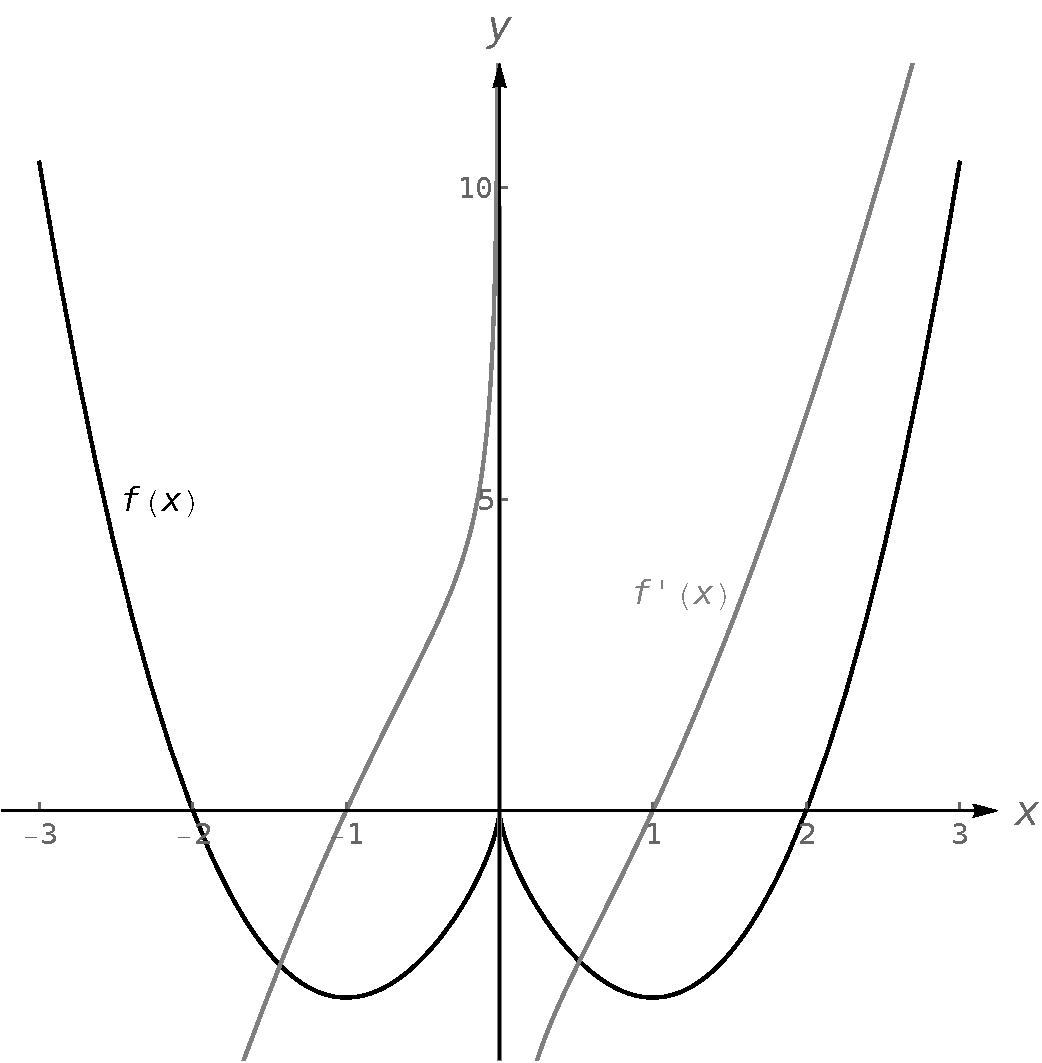
\includegraphics[width=0.5\textwidth]{fig_behaviour_15}
	\caption{A graph of $f(x)$ (black)  and $f'(x)$ (gray) in Example \ref{ex_incr3}, showing where $f$ is increasing and decreasing.}
	\label{fig_behaviour_15}
	\end{center}
\end{figure}

\end{example}

We have seen how the first derivative of a function helps determine when the function is going up or down. In the next section, we will see how the second derivative helps determine how the graph of a function curves.

\section{Concavity and the second derivative}\label{sec:concavity}

Our study of nice functions continues. The previous section showed how the first derivative of a function, \fp, can relay important information about $f$. We now apply the same technique to \fp\ itself, and learn what this tells us about $f$.

The key to studying $\fp$ is to consider its derivative, namely  $\fp'$, which is the second derivative of $f$.  When $\fp'\geq0$, $\fp$ is increasing. When $\fp'\leq0$, \fp\ is decreasing.  $\fp$ has relative maxima and minima where $\fp'=0$ or is undefined.

This section explores how knowing information about \fpp\ gives information about $f$.

\subsection{Concavity}

We begin with a definition, then explore its meaning.

\begin{definition}[Concave up and concave down]\label{def:concavity}
Let $f$ be differentiable on an interval $I$. 
\begin{enumerate}
    \item The graph of $f$ is \textbf{concave up} (\textit{convex}) on $I$ if $\fp$ is increasing. 
    \item The graph of $f$ is \textbf{concave down} (\textit{concaaf}) on $I$ if $\fp$ is decreasing. 
    \item If $\fp$ is constant then the graph of $f$ is said to have no \textbf{concavity} (\textit{concaviteit}).
    \end{enumerate}
\end{definition}
\index{concavity}\index{concave up}\index{concave down}
\index[aut]{convexiteit}\index[aut]{concaviteit}

Note that we often state that $f$ is concave up instead of the graph of $f$ is concave up for simplicity. Besides, in agreement with the terminology used for increasing and decreasing functions (Definition~\ref{def:incr_decr}), we call a function $f$ strictly concave up or down if $f'$ is strictly increasing or decreasing, respectively. 

The graph of a function $f$ is concave up when \fp\ is increasing. That means as one looks at a concave up graph from left to right, the slopes of the tangent lines will be increasing. Consider Figure \ref{fig_behaviour_16a}, where a concave up graph is shown along with some tangent lines. Notice how the tangent line on the left is  steep, downward, corresponding to a  small value of \fp. On the right, the tangent line is steep, upward, corresponding to a large value of \fp. If a function is decreasing and concave up, then its rate of decrease is slowing; it is levelling off.  If the  function is increasing and concave up, then the rate of increase is increasing. 

Now consider a function which is concave down. We essentially repeat the above paragraphs with slight variation. The graph of a function $f$ is concave down  when \fp\ is decreasing. That means as one looks at a concave down graph from left to right, the slopes of the tangent lines will be decreasing. Consider Figure \ref{fig_behaviour_16b}, where a concave down graph is shown along with some tangent lines. Notice how the tangent line on the left is  steep, upward, corresponding to a large value of \fp. On the right, the tangent line is steep, downward, corresponding to a small value of \fp. If a function is increasing and concave down, then its rate of increase is slowing; it is levelling off.  If the function is decreasing and concave down, then the {rate} of decrease is decreasing.  The function is decreasing at a faster and faster rate. Geometrically speaking it is clear that a function is concave up if its graph lies above its tangent lines. A function is concave down if its graph lies below its tangent lines.

\begin{figure}[H]
\centering
%\raisebox{0.5cm}{
\subfigure[\label{fig_behaviour_16a}]{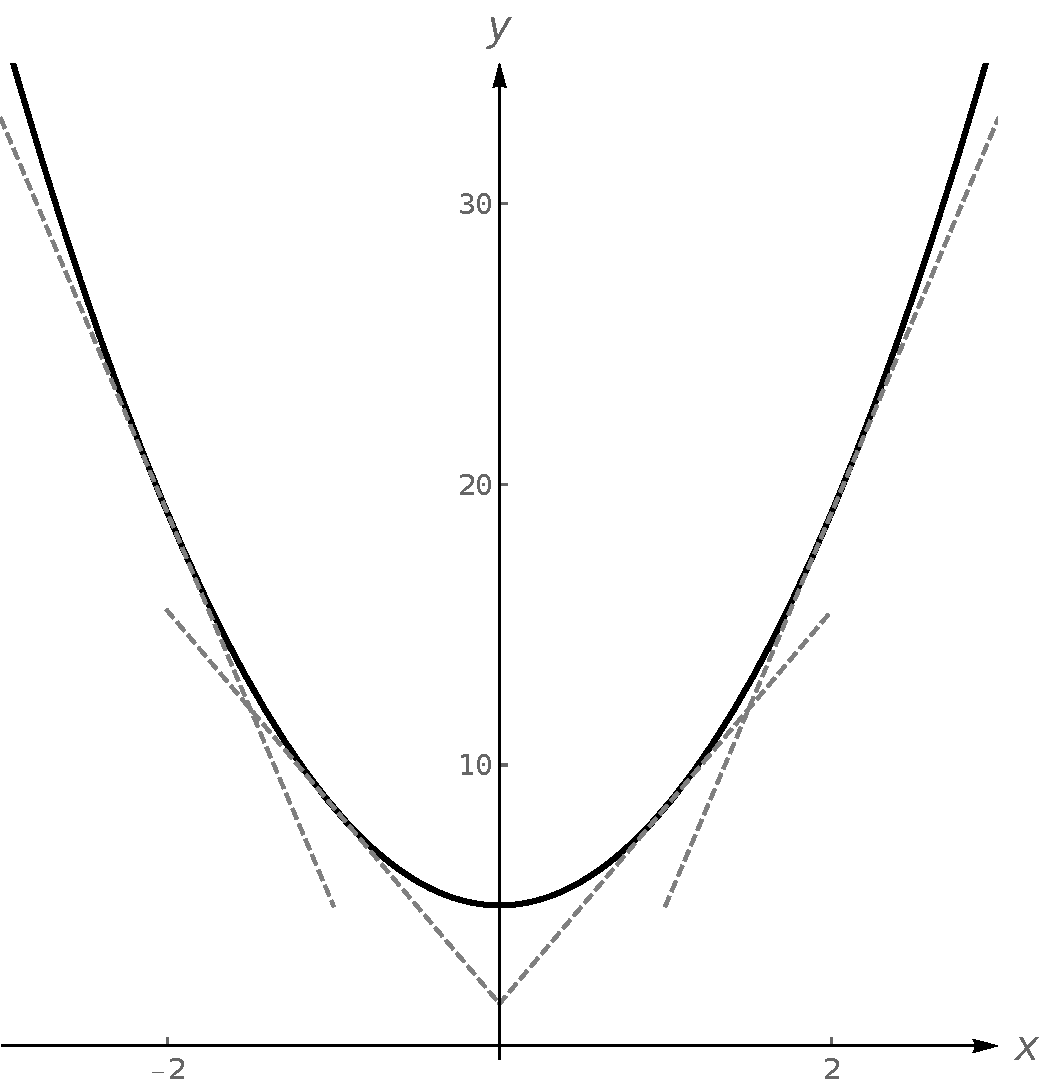
\includegraphics[width=0.35\textwidth]{fig_behaviour_16a}}
\qquad
\subfigure[\label{fig_behaviour_16b}]{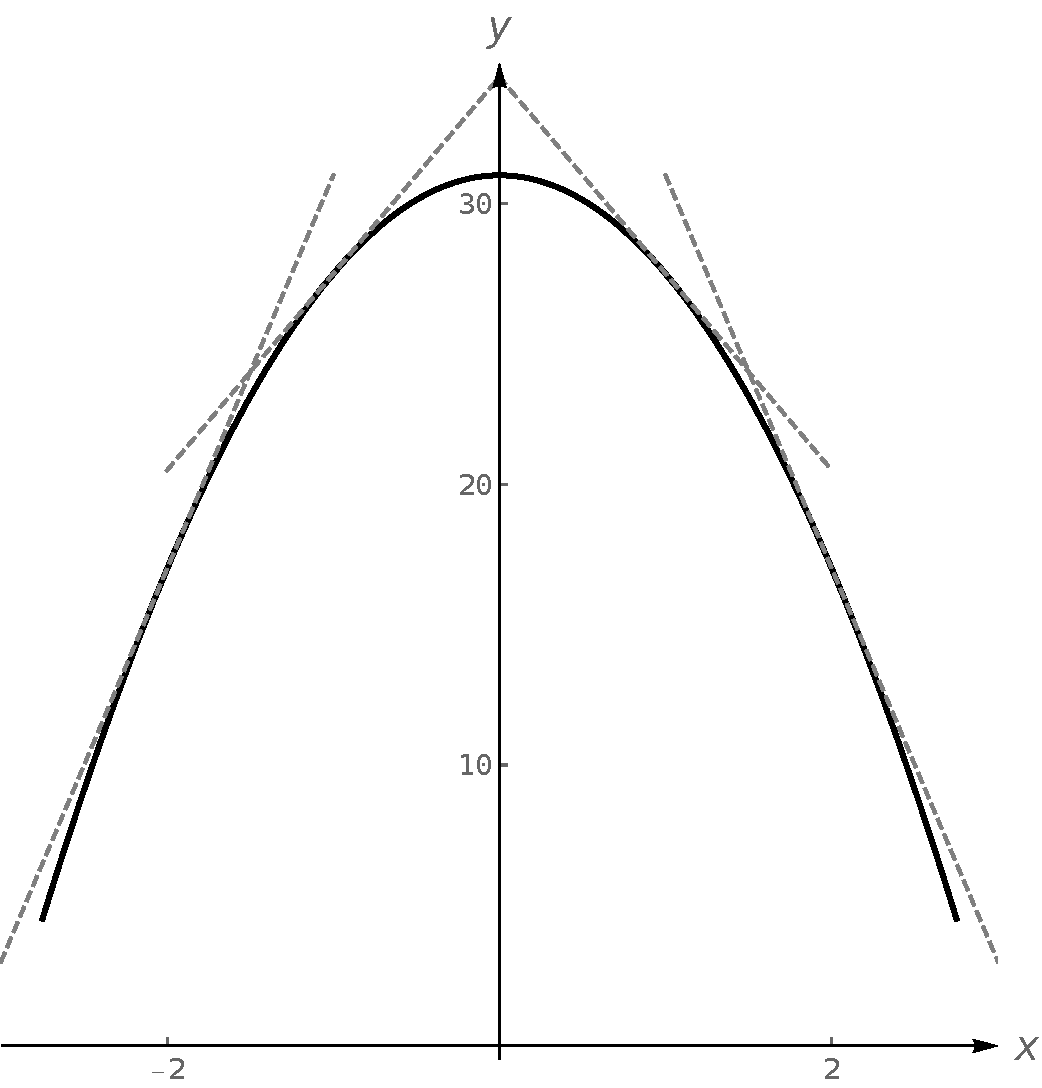
\includegraphics[width=0.35\textwidth]{fig_behaviour_16b}}
\caption{A function $f$ with a concave up (a) and concave down (b) graph together with some tangent lines (dashed). }
\end{figure}


Our definition of concave up and concave down is given in terms of when the first derivative is increasing or decreasing. We can apply the results of Section~\ref{sec:incr_decr} to find intervals on which a graph is concave up or down. That is, we recognize that $\fp$ is increasing when $\fpp\geq0$, etc. 

\pagebreak
\begin{theorem}[Test for concavity]\label{thm:concavity}
Let $f$ be twice differentiable on an interval $I$. The graph of $f$ is concave up if $\fpp\geq0$ on $I$, and is concave down if $\fpp\leq0$ on $I$. \index{concavity ! test}
\end{theorem}

\ifanalysis

\begin{proof}
We will only prove the concave up part of the theorem as the proof of the concave down part is nearly identical.

Let a be any number in the interval $I$. The tangent line to $f(x)$ at $x=a$ is,
$$
y =\ell(x)= f\left( a \right) + f'\left( a \right)\left( {x - a} \right)\,.
$$
To show that $f(x)$ is concave up on $I$ then we need to show that for any $x$, $x\neq a$, in $I$ that,
$$
f\left( x \right) > f\left( a \right) + f'\left( a \right)\left( {x - a} \right)\,,
$$
or in other words, the tangent line is always below the graph of $f(x)$ on $I$. Note that we require $x\neq a$ because at that point we know that $f(x)=f(a)$ since we are talking about the tangent line.  

Let us start the proof off by first assuming that $x>a$. Using the mean value theorem on $[a,x]$ means there is a number $c$ such that $a<c<x$ and,
$$
f\left( x \right) - f\left( a \right) = f'\left( c \right)\left( {x - a} \right)\,,
$$
or equivalently
\begin{equation}
f\left( x \right) = f\left( a \right) + f'\left( c \right)\left( {x - a} \right)\,. \label{eq:eq2}
\end{equation}
Next, let us use the fact that $f''(x)>0$ for every $x$ on $I$. This means that the first derivative, $f'(x)$, must be increasing. Now, we know from the mean value theorem that $a<c$ and so because $f'(x)$
is increasing we must have, 
\begin{equation}
f'\left( a \right) < f'\left( c \right)\,. \label{eq:eq3} 
\end{equation}


Recall as well that we are assuming x>a and so $x-a>0$. If we now multiply Inequality~\eqref{eq:eq3} by $x-a$ (which is positive and so the inequality stays the same) we get,
$$
f'\left( a \right)\left( {x - a} \right) < f'\left( c \right)\left( {x - a} \right)\,.
$$
However, by Equation~\eqref{eq:eq2}, the right side of this is nothing more than $f(x)-f(a)$ and so we have,
$$
f\left( a \right) + f'\left( a \right)\left( {x - a} \right) < f\left( x \right)\,,
$$
but this is exactly what we wanted to show. So, provided $x>a$ the tangent line is in fact below the graph of $f(x)$. 

We now need to assume $x<a$. Using the mean value theorem on $[x,a]$ means there is a number $c$ such that $x<c<a$ and
$$
f\left( a \right) - f\left( x \right) = f'\left( c \right)\left( {a - x} \right)\,.
$$
If we multiply both sides of this by $-1$ and then adding $f(a)$ to both sides and we again arrive at Equation~\eqref{eq:eq2}.

Now, from the mean value theorem we know that $c<a$
and because $f''(x)>0$ for every $x$ on $I$ we know that the derivative is still increasing and so we have, $f'(c)<f'(a)$. Let us now multiply this by $x-a$, which is now a negative number since $x<a$. This gives
$$
f'\left( c \right)\left( {x - a} \right) > f'\left( a \right)\left( {x - a} \right)\,.
$$
Notice that we had to switch the direction of the inequality since we were multiplying by a negative number. If we now add $f(a)$ to both sides of this and then substitute Equation~\eqref{eq:eq2} into the results we arrive at,
\begin{align*}
f\left( a \right) + f'\left( c \right)\left( {x - a} \right) & > f\left( a \right) + f'\left( a \right)\left( {x - a} \right)\\ 
 \Leftrightarrow \qquad  \quad f\left( x \right) &> f\left( a \right) + f'\left( a \right)\left( {x - a} \right)
\end{align*}

So, again we have shown that the tangent line is always below the graph of $f(x)$. We have now shown that if $x$ is any number in $I$, with $x\neq a$ the tangent lines are always below the graph of $f(x)$ on $I$ and so $f(x)$ is concave up on $I$.

% http://tutorial.math.lamar.edu/Classes/CalcI/DerivativeAppsProofs.aspx#Extras_DerAppPf_SDT
\phantom{}
\end{proof}

\fi

Figure~\ref{fig_behaviour_17} demonstrates the four ways that concavity interacts with increasing/decreasing, along with the relationships with the first and second derivatives.

\begin{figure}[h]
	\begin{center}
			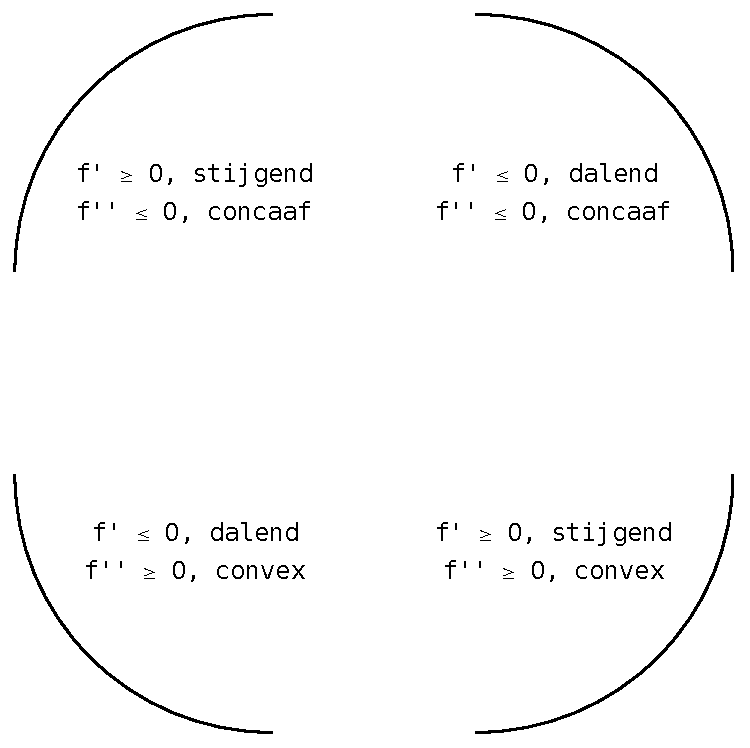
\includegraphics[width=0.5\textwidth]{fig_behaviour_17}
	\caption{Demonstrating the 4 ways that concavity interacts with increasing/decreasing, along with the relationships with the first and second derivatives.}
	\label{fig_behaviour_17}
	\end{center}
\end{figure}


If knowing where a graph is concave up/down is important, it makes sense that the places where the graph changes from one to the other is also important. This leads us to a definition.

\begin{definition}[Point of inflection]\label{def:infl}
A \textbf{point of inflection} (\textit{buigpunt}) is a point on the graph of $f$ at which the concavity of $f$ changes.\index{point of inflection}
\end{definition}
\index{inflection point}\index[aut]{buigpunt}

If the concavity of $f$ changes at a point $(c,f(c))$, then \fp\ is changing from increasing to decreasing (or, decreasing to increasing) at $x=c$. That means that the sign of \fpp\ is changing from positive to negative (or, negative to positive) at $x=c$.  This leads to the following theorem.

\begin{theorem}[Points of inflection]\label{thm:inflection}
If $(c,f(c))$ is a point of inflection on the graph of $f$, then either $\fpp(c)=0$ or $\fpp$ is not defined at $c$.
\end{theorem}

We have identified the concepts of concavity and points of inflection. It is now time to practice using these concepts; given a function, we should be able to find its points of inflection and identify intervals on which it is concave up or down. We do so in the following example.

\begin{example}\label{ex_conc2}
Let 
$$f(x)=\dfrac{x}{x^2-1}.$$
Find the inflection points of $f$ and the intervals on which it is concave up/down.


\xhrulefill{gray}{2.5pt}Solution \xhrulefill{gray}{2.5pt}

We need to find \fp\ and \fpp. Using the quotient rule and simplifying, we find
$$\fp(x)=\frac{-(1+x^2)}{(x^2-1)^2} \quad \text{and}\quad \fpp(x) = \frac{2x(x^2+3)}{(x^2-1)^3}.$$

To find the possible points of inflection, we seek to find where $\fpp(x)=0$ and where $\fpp$ is not defined. Solving $\fpp(x)=0$ reduces to solving $2x(x^2+3)=0$; we find $x=0$.  We find that \fpp\ is not defined when $x=\pm 1$, for then the denominator of \fpp\ is 0. We also note that $f$ itself is not defined at $x=\pm1$, having a domain of $\left.\right]-\infty,-1\left[\right.\cup\left.\right]-1,1\left[\right.\cup\left.\right]1,+\infty\left[\right.$. Since the domain of $f$ is the union of three intervals, it makes sense that the concavity of $f$ could switch across intervals. We technically cannot say that $f$ has a point of inflection at $x=\pm1$ as they are not part of the domain, but we must still consider these $x$-values to be important and will include them in our number line.

The important $x$-values at which concavity might switch are $x=-1$, $x=0$ and $x=1$, which  split the number line into four intervals.



 We determine the concavity on each. Keep in mind that all we are concerned with is the sign of \fpp\ on the interval.

\begin{description}
\item \textbf{Interval 1: $\left.\right]-\infty,-1\left[\right.$}

Select a number $c$ in this interval with a large magnitude (for instance, $c=-100$). The denominator of $\fp'(x)$ will be positive. In the numerator, the $(c^2+3)$ will be positive and the $2c$ term will be negative. Thus the numerator is negative and $\fpp(c)$ is negative. We conclude $f$ is concave down on $\left.\right]-\infty,-1\left[\right.$.

\item \textbf{Interval 2: $\left.\right]-1,0\left[\right.$} 

 For any number $c$ in this interval, the term $2c$ in the numerator will be negative, the term $(c^2+3)$ in the numerator will be positive, and the term $(c^2-1)^3$ in the denominator will be negative. Thus $\fpp(c)>0$ and $f$ is concave up on this interval.

\item\textbf{Interval 3: $\left.\right]0,1\left[\right.$} 

Any number $c$ in this interval will be positive and small. Thus the numerator is positive while the denominator is negative. Thus $\fpp(c)<0$ and $f$ is concave down on this interval.

\item\textbf{Interval 4: $\left.\right]1,+\infty\left[\right.$} 

Choose a large value for $c$. It is evident that $\fpp(c)>0$, so we conclude that $f$ is concave up on $\left.\right]1,+\infty\left[\right.$.

\end{description}
Since, we get
	\begin{center}
			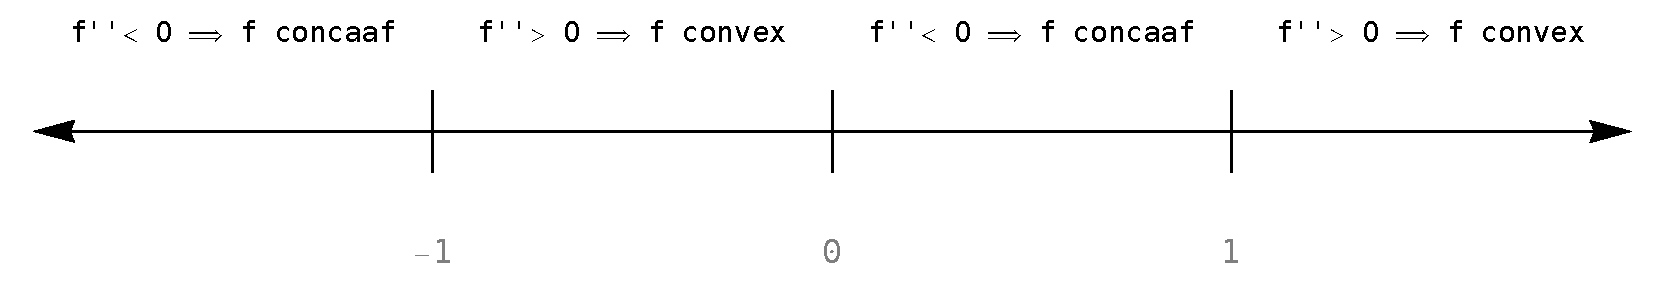
\includegraphics[width=0.8\textwidth]{fig_behaviour_18}
	\end{center}
	
we conclude that $f$ is concave up on $\left.\right]-1,0\left[\right.$ and $\left.\right]1,+\infty\left[\right.$ and concave down on $\left.\right]-\infty,-1\left[\right.$ and $\left.\right]0,1\left[\right.$. There is only one point of inflection, $\left.\right]0,0\left[\right.$, as $f$ is not defined at $x=\pm 1$. Our work is confirmed by the graph of $f$ in Figure~\ref{fig_behaviour_19}. 


\begin{figure}[H]
	\begin{center}
			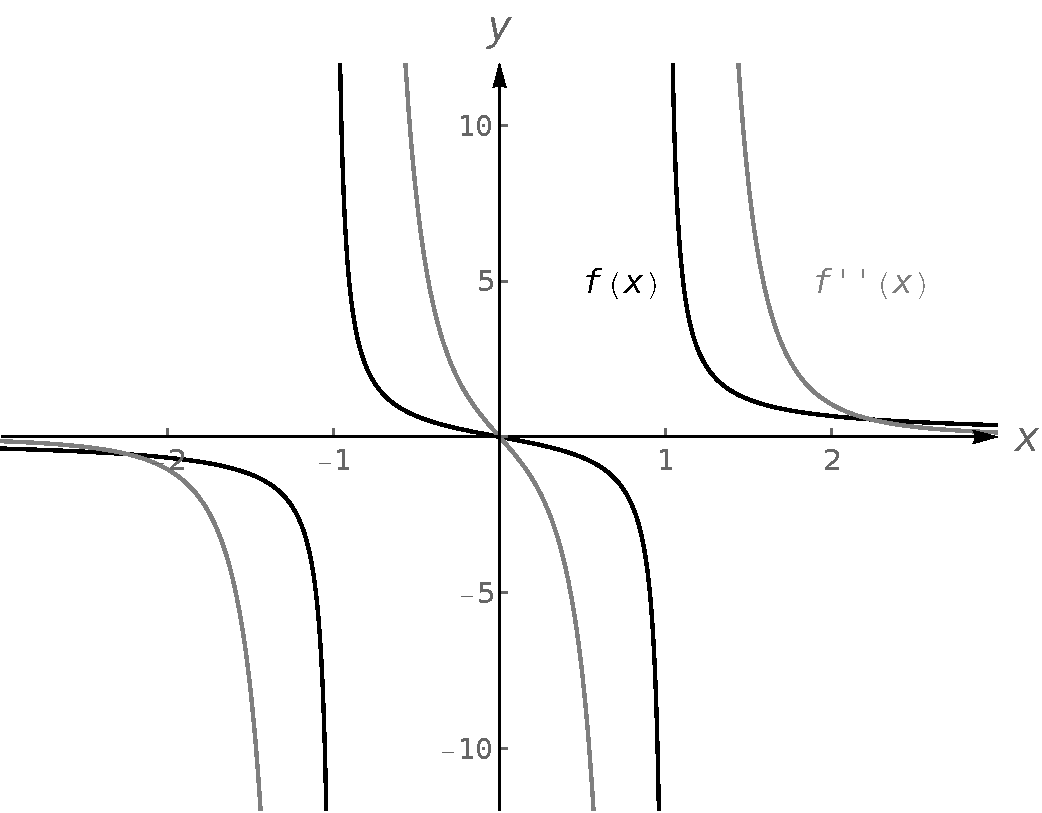
\includegraphics[width=0.5\textwidth]{fig_behaviour_19}
	\caption{A graph of $f(x)$ (black) and $\fpp(x)$ (gray) in Example \ref{ex_conc2}.}
	\label{fig_behaviour_19}
	\end{center}
\end{figure}


\end{example}

Recall that relative maxima and minima of $f$ are found at critical points of $f$; that is, they are found when $\fp(x)=0$ or when $\fp$ is undefined. Likewise, the relative maxima and minima of \fp\ are found when $\fpp(x)=0$ or when \fpp\ is undefined; note that these are the inflection points of $f$. 

What does a relative maximum of \fp\  mean? The derivative measures the rate of change of $f$; maximizing \fp\ means finding  where $f$ is increasing the most -- where $f$ has the steepest tangent line. A similar statement can be made for minimizing \fp; it corresponds to where $f$ has the steepest negatively--sloped tangent line.

We utilize this concept in the next example.

\begin{example}\label{ex_conc3}
The sales of a certain product over a three-year span are modelled by $S(t)= t^4-8t^2+20$, where $t$ is the time in years.  Over the first two years, sales are decreasing.  Find the point at which sales are decreasing at their greatest rate.

\xhrulefill{gray}{2.5pt}Solution \xhrulefill{gray}{2.5pt}


We want to maximize the rate of decrease, which is to say, we want to find where $S'$ has a minimum.  To do this, we find where $S''$ is 0.  We find $S'(t)=4t^3-16t$ and $S''(t)=12t^2-16$.  Setting $S''(t)=0$ and solving, we get $t=\sqrt{4/3}\approx 1.16$. Note that we ignore the negative value of $t$ since it does not lie in the domain of our function $S$.

This is both the inflection point and the point of maximum decrease.  This is the point at which things first start looking up for the company.  After the inflection point, it will still take some time before sales start to increase, but at least sales are not decreasing quite as quickly as they had been.

A graph of $S(t)$ and $S'(t)$ is given in Figure~\ref{fig_behaviour_20}. When $S'(t)<0$, sales are decreasing; note how at $t\approx 1.16$, $S'(t)$ is minimized. That is, sales are decreasing at the fastest rate at $t\approx 1.16$.  On the interval of $(1.16,2)$, $S$ is decreasing but concave up, so the decline in sales is levelling off.

\begin{figure}[H]
	\begin{center}
			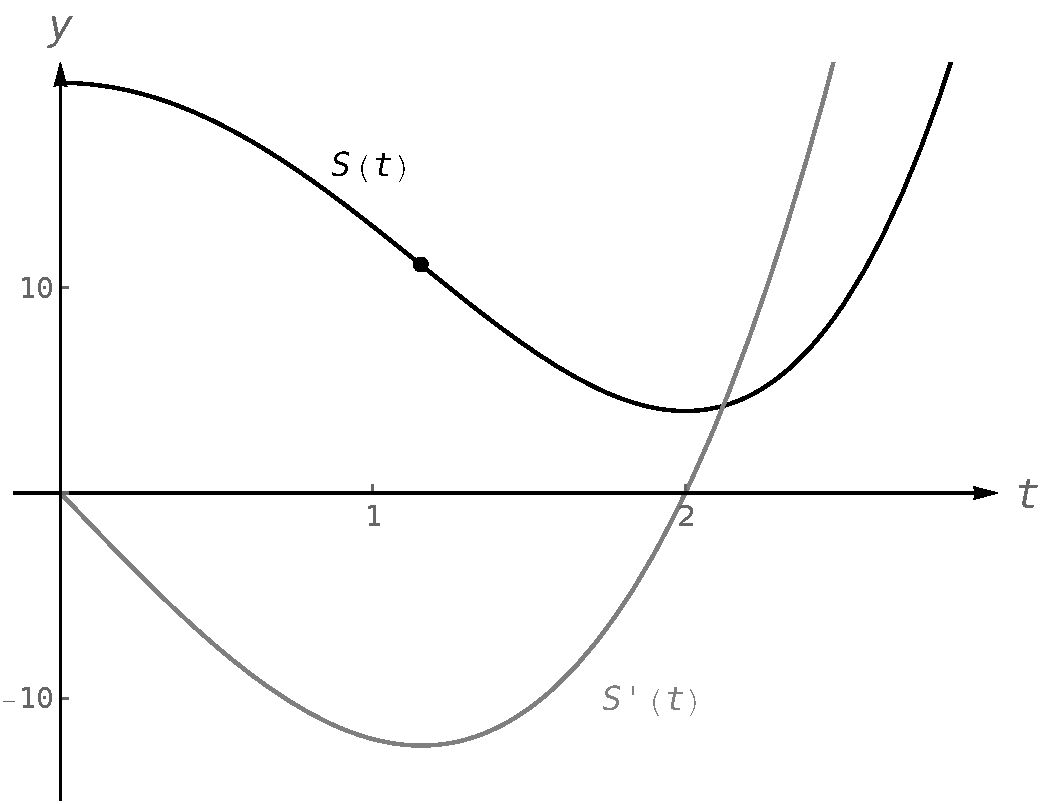
\includegraphics[width=0.5\textwidth]{fig_behaviour_20}
	\caption{A graph of $S(t)$ (black) in Example \ref{ex_conc3} along with $S'(t)$ (gray).}
	\label{fig_behaviour_20}
	\end{center}
\end{figure}

\end{example}

Not every critical point corresponds to a relative extrema; $f(x)=x^3$ has a critical point at $(0,0)$ but no relative maximum or minimum (Figure~\ref{fig_behaviour_3}). Likewise, just because $\fpp(x)=0$ we cannot conclude concavity changes at that point. We were careful before to use terminology possible point of inflection since we needed to check to see if the concavity changed. The canonical example of $\fpp(x)=0$ without concavity changing is $f(x)=x^4$. At $x=0$, $\fpp(x)=0$ but $f$ is always concave up, as shown in Figure \ref{fig_behaviour_21}.

\begin{figure}[H]
	\begin{center}
			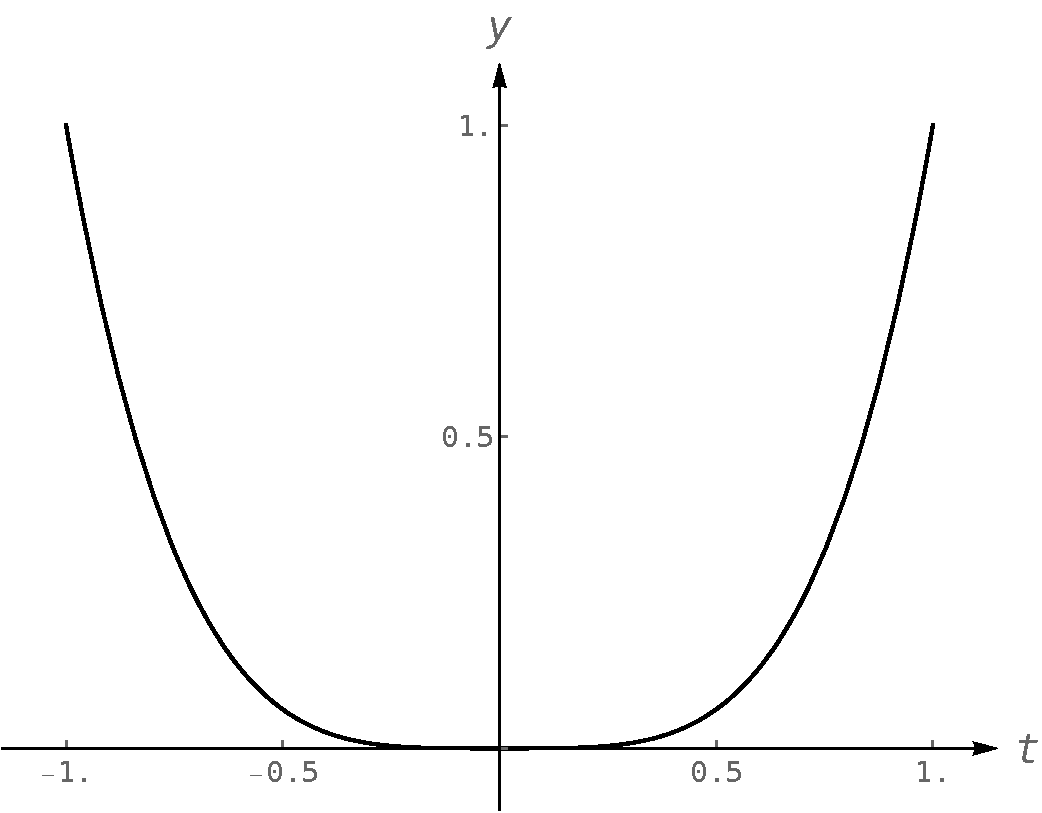
\includegraphics[width=0.5\textwidth]{fig_behaviour_21}
	\caption{A graph of $f(x) = x^4$.}
	\label{fig_behaviour_21}
	\end{center}
\end{figure}

\subsection{The second derivative test}


The first derivative of a function gave us a test to find if a critical value corresponded to a relative maximum, minimum, or neither. The second derivative gives us another way to test if a critical point is a local maximum or minimum. The following theorem states something that is intuitive: if a critical value occurs in a region where a function $f$ is concave up, then that critical value must correspond to a relative minimum of $f$, etc (Figure~\ref{fig_behaviour_22}).

\begin{figure}[h]
	\begin{center}
			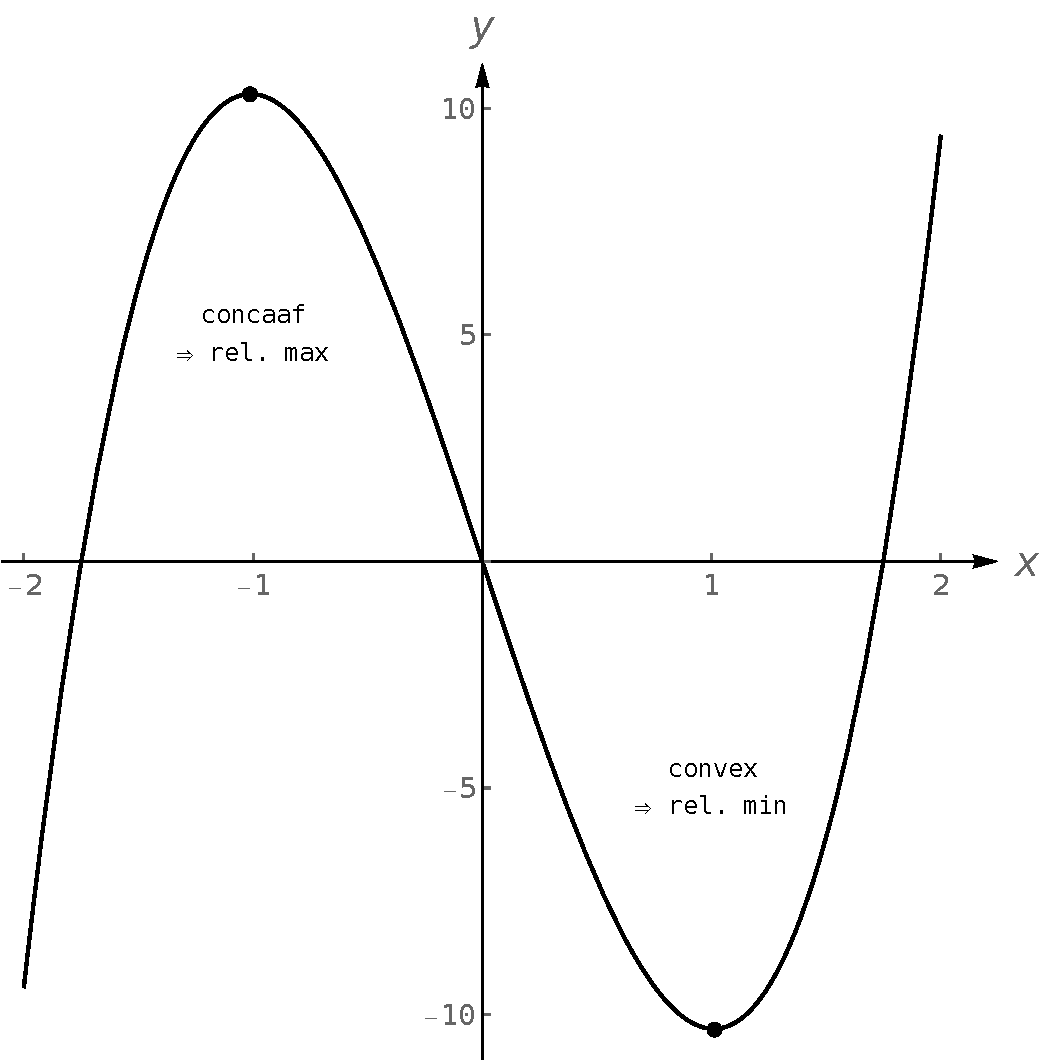
\includegraphics[width=0.5\textwidth]{fig_behaviour_22}
	\caption{Demonstrating the second derivative test.}
	\label{fig_behaviour_22}
	\end{center}
\end{figure}

\begin{theorem}[The second derivative test]\label{thm:second_der}%
 Let $c$ be a critical value of $f$ where  $\fpp(c)$ is defined. \index{second derivative test}
\begin{enumerate}
\item If $\fpp(c)<0$, then $f$ has a local maximum at $(c,f(c))$.
\item If $\fpp(c)>0$, then $f$ has a local minimum at $(c,f(c))$.
\item If $f''(c)=0$ then $x=c$ can be a local maximum, relative minimum or neither.
\end{enumerate}
\end{theorem}

\ifanalysis

\begin{proof}
First let us assume that $f''(x)$ is continuous in a region around $x=c$, so that we can assume that in fact $f''(c)<0$ is also true in some open region, say $]a,b[$ around $x=c$, i.e. $a<c<b$.

Now let $x$ be any number such that $a<x<c$, we are going to use the mean value theorem on $[x,c]$. However, instead of using it on the function itself we are going to use it on the first derivative. So, the mean value theorem tells us that there is a number $d$ for which $x<d<c$ such that,
$$
f'\left( c \right) - f'\left( x \right) = f''\left( d \right)\left( {c - x} \right)\,.
$$
Now, because $a<x<d<c$ we know that $f''(d)<0$ and we also know that $c-x>0$, so we then get that 
$f'(c)-f'(x)<0$. However, we also assumed that $f'(c)=0$ and so we have that $f'(x)>0$. Or, in other words to the left of $x=c$ the function is increasing.

Let us now turn things around and let $x$
be any number such that  $c<x<b$ and use the mean value theorem on $[c,x]$ and the first derivative. The mean value theorem tells us that there is a number $c<d<x$ such that,
$$
f'\left( x \right) - f'\left( c \right) = f''\left( d \right)\left( {x - c} \right)\,.
$$

Now, because $c<d<x<b$ we know that $f''(d)<0$ and we also know that $x-c>0$ so we then get that 
$f'(x)-f'(c)<0$.  Again, use the fact that we also assumed that $f'(c)=0$ to get $f'(x)<0$. Consequently, we now know that to the right of $x=c$
the function is decreasing.

So, to the left of $x=c$ the function is increasing and to the right of $x=c$ the function is decreasing so by the first derivative test this means that $x=c$ must be a relative maximum.
\end{proof}

\fi

The second derivative test relates to the first derivative test in the following way. If $\fpp(c)>0$, then the graph is concave up at a critical point $c$ and $\fp$ itself is growing.  Since $\fp(c)=0$ and $\fp$ is growing at $c$, then it must go from negative to positive at $c$.  This means the function goes from decreasing to increasing, indicating a local minimum at $c$.
%\clearpage

\begin{example}\label{ex_conc4}
Let 
$$f(x)=\dfrac{100}{x} + x.$$
Find the critical points of $f$ and label them as relative maxima or minima.

\xhrulefill{gray}{2.5pt}Solution \xhrulefill{gray}{2.5pt}

We find 
$$\fp(x)=-\dfrac{100}{x^2}+1$$
and 
$$\fpp(x) = \dfrac{200}{x^3}.$$  We set $\fp(x)=0$ and solve for $x$ to find the critical values. Note that \fp\ is not defined at $x=0$, but neither is $f$ so this is not a critical value. We find  the critical values are $x=\pm 10$.  Evaluating \fpp\ at $x=10$ gives $0.2>0$, so there is a local minimum at $x=10$.  Evaluating $\fpp(-10)=-0.2<0$, determining a relative maximum at  $x=-10$. These results are confirmed in Figure \ref{fig_behaviour_23}.

\begin{figure}[H]
	\begin{center}
			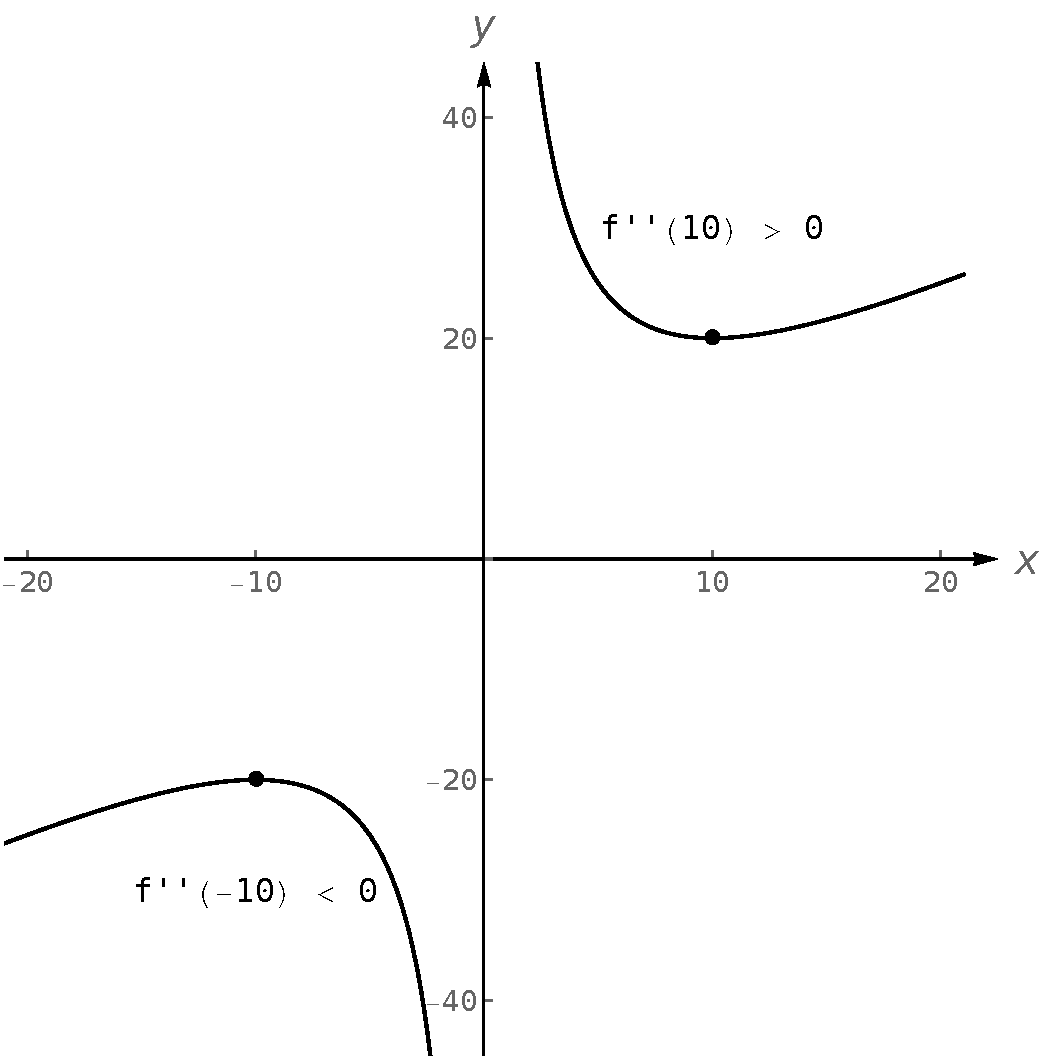
\includegraphics[width=0.5\textwidth]{fig_behaviour_23}
	\caption{A graph of $f(x)=100/x + x$ in Example~\ref{ex_conc4}.}
	\label{fig_behaviour_23}
	\end{center}
\end{figure}

\end{example}

We have been learning how the first and second derivatives of a function relate information about the graph of that function. We have found intervals of increasing and decreasing, intervals where the graph is concave up and down, along with the locations of relative extrema and inflection points. In Chapter~\ref{chap_limits} we saw how limits explained asymptotic behaviour. In the next section we combine all of this information to produce accurate sketches of functions.



\section{Curve sketching}\label{sec:sketch}


We have been learning how we can understand the behaviour of a function based on its first and second derivatives. While we have been treating the properties of a function separately, we combine them here to produce an accurate graph of the function without plotting lots of extraneous points.
\ifmathematica
Why bother? Graphing utilities are very accessible, whether on a computer, a hand--held calculator, or a smartphone. These resources are usually very fast and accurate. For instance, remember that we can plot an explicitly defined function in Mathematica using the built-in command \lstinline{Plot}, while \lstinline{ContourPlot} may be used to plot implicitly defined functions (see Chapter~\ref{chap_functions}).   We will see that our method is not particularly fast -- it will require time. 
\fi
\ifpython
Why bother? Graphing utilities are very accessible, whether on a computer, a hand--held calculator, or a smartphone. These resources are usually very fast and accurate. For instance, remember that we can plot an explicitly defined function in Python using the built-in command \lstinline{Plot}, while \lstinline{ContourPlot} may be used to plot implicitly defined functions (see Chapter~\ref{chap_functions}).   We will see that our method is not particularly fast -- it will require time. 
\fi
We are attempting to understand the behavior of a function $f$ based on the information given by its derivatives. While all of a function's derivatives relay information about it, it turns out that most of the behaviour we care about is explained by \fp\ and \fpp. Understanding the interactions between the graph of $f$ and \fp\ and \fpp\ is important. To gain this understanding, one might argue that all that is needed is to look at lots of graphs. This is true to a point, but is somewhat similar to stating that one understands how an engine works after looking only at pictures. It is true that the basic ideas will be conveyed, but hands--on access increases understanding.

To produce an accurate sketch of a given function $f$, take  the following steps.\index{curve sketching}\index[aut]{functie-onderzoek}

\begin{enumerate}
\item		Find the domain of $f$. Generally, we assume that the domain is the entire real line then find restrictions, such as where a denominator is 0 or where negatives appear under the radical.
\item Find symmetries and intercepts.
\item		Find the location of any asymptotes of $f$:
\begin{enumerate}
\item vertical
\item horizontal 
\item slant asymptotes
\end{enumerate}
\item		Find the critical and singular points of $f$.
\item		Find the possible points of inflection of $f$.
\item		Create a number line that includes all critical points, possible points of inflection, and locations of vertical asymptotes. For each interval created, determine whether $f$ is increasing or decreasing, concave up or down.
\item		Evaluate $f$ at each critical point and possible point of inflection. Plot these points on a set of axes. Connect these points with curves exhibiting the proper concavity. Sketch asymptotes and $x$- and $y$-intercepts where applicable.
\end{enumerate}

\begin{example}\label{ex_sketch1}
Sketch $f(x) = 3x^3-10x^2+7x+5$.

\xhrulefill{gray}{2.5pt}Solution \xhrulefill{gray}{2.5pt}

We follow the steps outlined above.
\begin{enumerate}
\item		The domain of $f$ is the entire real line; there are no values $x$ for which $f(x)$ is not defined.
\item It can be verified easily that the function is neither even nor odd. Besides, the $x$-intercept is about $x=-0.424$ while the $y$-intercept is $y=5$.
\item \begin{enumerate}
\item		There are no vertical asymptotes.
\item		We determine the end behaviour using limits as $x$ approaches $\pm \infty$.				
			$$\lim_{x\to -\infty} f(x) = -\infty \qquad \text{and} \qquad \lim_{x\to +\infty}f(x) = +\infty$$
			So, we do not have any horizontal asymptotes.
\item There is no slant asymptote since
$$
a=\lim_{x\to \pm\infty} \dfrac{f(x)}{x}=\lim_{x\to \pm\infty}\left(3x^2-10x+7+\frac{5}{x}\right)=+\infty.
$$
\end{enumerate}
\item		Find the critical values of $f$. We compute $\fp(x) = 9x^2-20x+7$. Use the quadratic formula to find the roots of $\fp$:
				$$x = \frac{20\pm \sqrt{(-20)^2-4(9)(7)}}{2(9)} = \frac19\left(10\pm\sqrt{37}\right),$$
so we have $x\approx 0.435$ or $x\approx 1.787.$
\item		Find the possible points of inflection of $f$. Compute $\fpp(x) = 18x-20$. We have $$\fpp(x) = 0 \quad\Rightarrow\quad x= \dfrac{10}{9}\approx 1.111.$$

\item		We place the values $x=(10\pm\sqrt{37})/9$ and $x=10/9$ on a number line and we mark each interval as increasing or decreasing, concave up or down:

	\begin{center}
			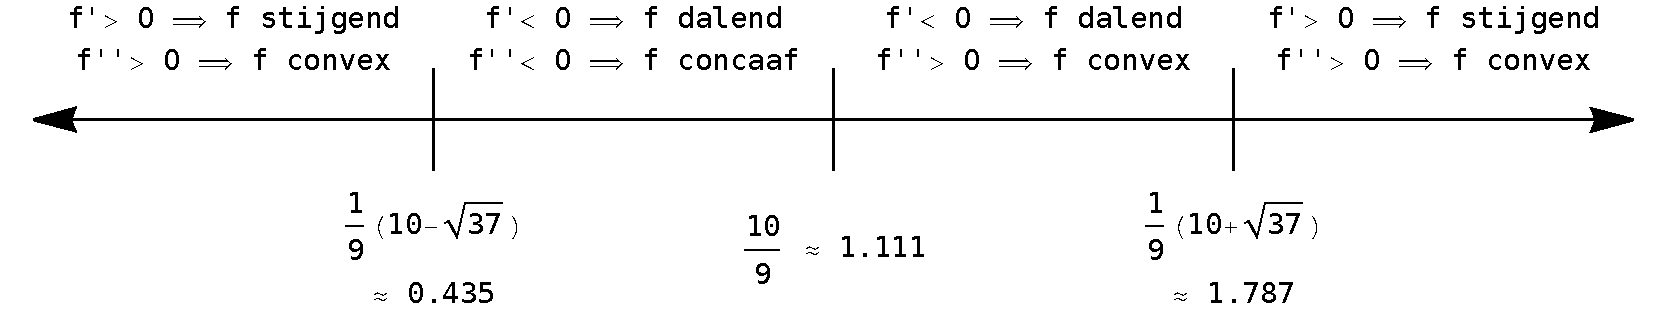
\includegraphics[width=0.8\textwidth]{fig_behaviour_24}
	\end{center}
	
\item		We now plot the appropriate points  and connect the points in such a way that the proper concavity is demonstrated. Our curve crosses the $y$-axis at $y=5$ and crosses the $x$-axis near $x=-0.424$ (Figure~\ref{fig_behaviour_25}). 
\end{enumerate}

\begin{figure}[H]
	\begin{center}
			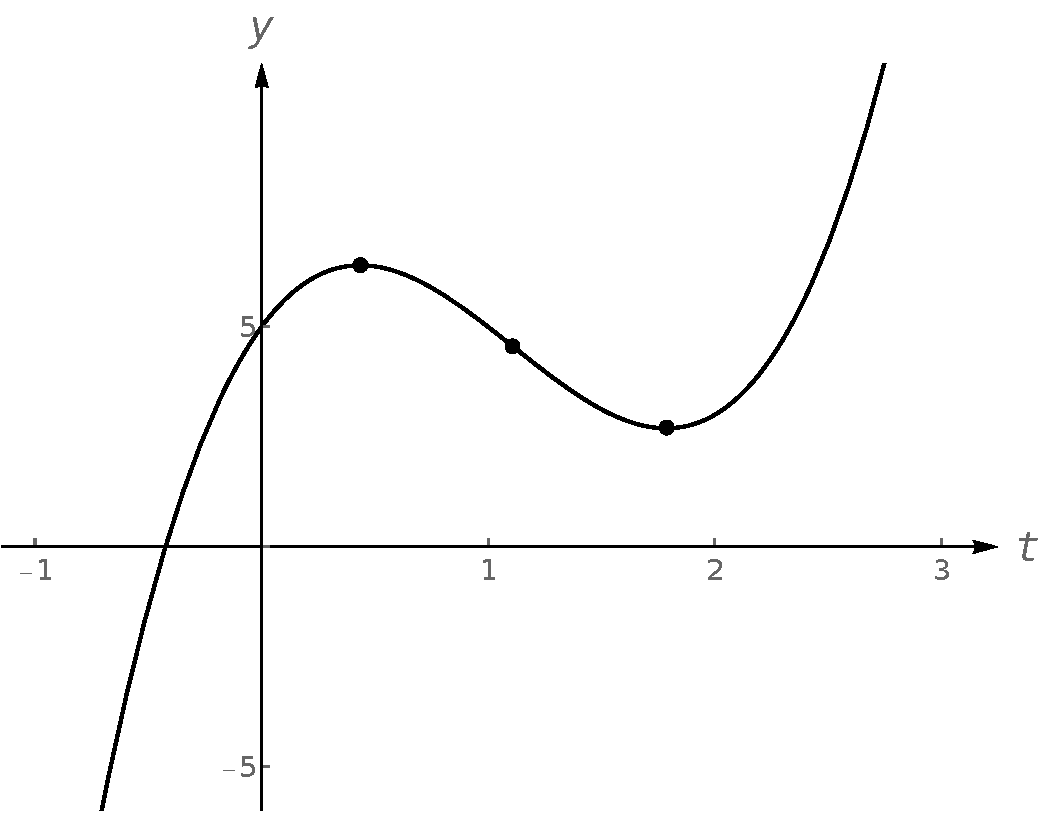
\includegraphics[width=0.5\textwidth]{fig_behaviour_25}
	\caption{A sketch of $f(x)= 3x^3-10x^2+7x+5$ in Example~\ref{ex_sketch1}.}
	\label{fig_behaviour_25}
	\end{center}
\end{figure}

\end{example}

\begin{example}\label{ex_sketch2}
Sketch 
$$\ds f(x) = \frac{x^2-x-2}{x^2-x-6}.$$

\xhrulefill{gray}{2.5pt}Solution \xhrulefill{gray}{2.5pt}

We again follow the steps outlined above.

\begin{enumerate}
		\item	In determining the domain, we assume it is all real numbers and look for restrictions. We find that at $x=-2$ and $x=3$, $f(x)$ is not defined because the denominator of $f(x)$ is 0 at those points. So, 
		$$\dom\,f = \{\text{real numbers } x\ | \ x\neq -2,3\}\,.$$
\item It can be verified easily that the function is neither even nor odd. Besides, the $x$-intercepts are $x=-1$ and $x=2$ while the $y$-intercept is $y=1/3$.

\item \begin{enumerate}
\item			The vertical asymptotes of $f$ are at $x=-2$ and $x=3$, the places where $f$ is undefined and the numerator of $f(x)$ is not zero.
		
		\item		There is a horizontal asymptote of $y=1$, as $\ds \lim_{x\to -\infty}f(x) = 1$ and $\ds\lim_{x\to+\infty}f(x) =1$.
		\item There are no slant asymptotes because there are already horizontal ones. 
\end{enumerate}
		\item		To find the critical values of $f$, we first find $\fp(x)$. Using the quotient rule, we find $$\fp(x) = \frac{-8x+4}{(x^2+x-6)^2} = \frac{-8x+4}{(x-3)^2(x+2)^2}.$$
		
		$\fp(x) = 0$ when $x = 1/2$, and $\fp$ is undefined when $x=-2$ or $x=3$. Since \fp\ is undefined only when $f$ is, these are not singular values. The only critical value is $x=1/2$.
		
		\item		To find the possible points of inflection, we find $\fpp(x)$, again employing the Quotient Rule: $$\fpp(x) = \frac{24x^2-24x+56}{(x-3)^3(x+2)^3}.$$
		
		We find that $\fpp(x)$ is never 0 (setting the numerator equal to 0 and solving for $x$, we find the only roots to this quadratic are complex) and \fpp\ is undefined when $x=-2$ or $x=3$. Thus concavity will possibly only change at $x=-2$ and $x=3$.
		

		\item		We place the values $x=1/2$, $x=-2$ and $x=3$ on a number line and we mark in each interval whether $f$ is increasing or decreasing, concave up or down:
		
	\begin{center}
			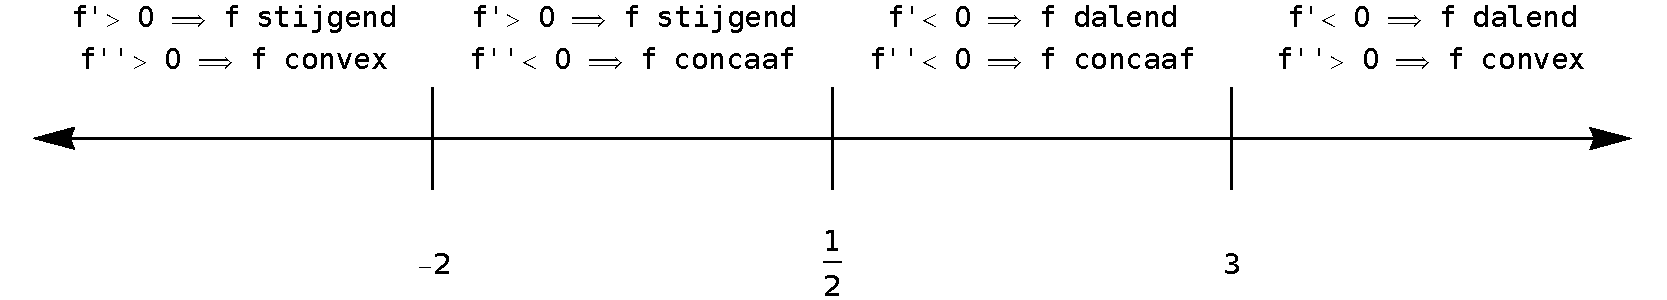
\includegraphics[width=0.8\textwidth]{fig_behaviour_26}
	\end{center}
	
	
		We see that $f$ has a relative maximum at $x=1/2$; concavity changes only at the vertical asymptotes.
		
		\item		In Figure \ref{fig_behaviour_27}, we plot the points from the number line on a set of axes and connect them in such a way that we get the appropriate concavity. We also show $f$ crossing the $x$-axis at $x=-1$ and $x=2$.
\end{enumerate}

\begin{figure}[H]
	\begin{center}
			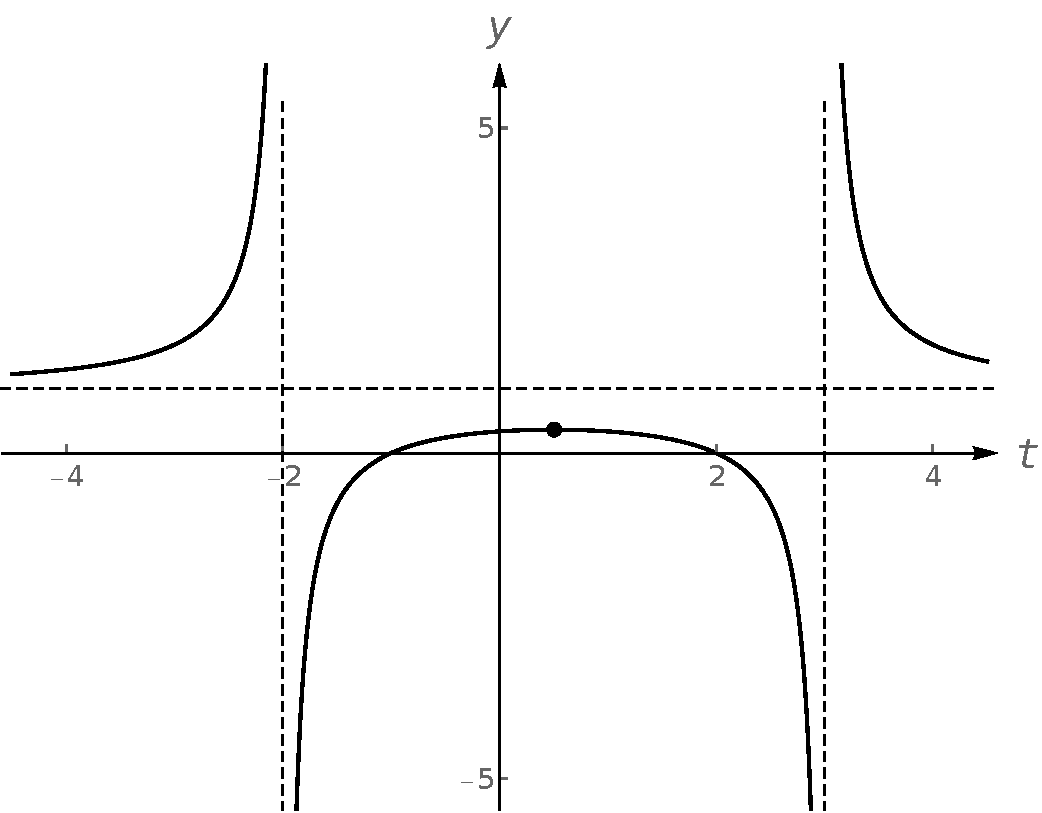
\includegraphics[width=0.45\textwidth]{fig_behaviour_27}
	\caption{A sketch of $f(x) = \frac{x^2-x-2}{x^2-x-6}$ in Example~\ref{ex_sketch2}.}
	\label{fig_behaviour_27}
	\end{center}
\end{figure}

\end{example}


%\begin{example}\label{ex_sketch3}
%Sketch 
%$$\ds f(x) = \frac{5(x-2)(x+1)}{x^2+2x+4}.$$

%\xhrulefill{gray}{2.5pt}Solution \xhrulefill{gray}{2.5pt}


%We again follow the same steps as before.
%	\begin{enumerate}
%	\item		We assume that the domain of $f$ is all real numbers and consider restrictions. The only restrictions come when the denominator is 0, but this never occurs. Therefore the domain of $f$ is all real numbers, $\mathbb{R}$.
%	\item It can be verified easily that the function is neither even nor odd. Besides, the $x$-intercept are $x=-1$ and $x=2$ while the $y$-intercept is $y=-5/2$.
%		\item\begin{enumerate}		
%	\item		There are no vertical asymptotes.
%	\item		We have a horizontal asymptote of $y=5$, as $\ds \lim_{x\to-\infty}f(x) = \lim_{x\to+\infty}f(x) = 5$.
%	\item There are no slant asymptotes because there are already horizontal ones. 
%	\end{enumerate}
%	\item		We find the critical values of $f$ by setting $\fp(x)=0$ and solving for $x$. We find 
%				$$\fp(x) = \frac{15x(x+4)}{(x^2+2x+4)^2}. $$
%	Consequently, we find $\fp(x) = 0$ when  $x=-4$ or $x=0$.			
%	\item		We find the possible points of inflection by solving $\fpp(x) = 0$ for $x$. We find
%			$$\fpp(x) = -\frac{30x^3+180x^2-240}{(x^2+2x+4)^3} .$$ The cubic in the numerator does not factor very nicely. We instead approximate the roots at $x= -5.759$, $x=-1.305$ and $x=1.064$.

%	\item		We place the critical points and possible points on a number line and mark each interval as increasing/decreasing, concave up/down appropriately:
	
			
%	\begin{center}
%			\includegraphics[width=0.95\textwidth]{fig_behaviour_21a}
%	\end{center}
	
%	\item		In Figure \ref{fig_behaviour_21b} we plot the significant points from the number line as well as the two roots of $f$, $x=-1$ and $x=2$, and connect the points with the proper concavity. 
%	\end{enumerate}

%\begin{figure}[H]
%	\begin{center}
%			\includegraphics[width=0.5\textwidth]{fig_behaviour_21b}
%	\caption{A sketch of $f(x) =  \frac{5(x-2)(x+1)}{x^2+2x+4}$ in Example~\ref{ex_sketch3}.}
%	\label{fig_behaviour_21b}
%	\end{center}
%\end{figure}

%\end{example}
\ifmathematica
Now why are computer graphics so good at curve sketching? It is not because computers are smarter than we are. Rather, it is largely because computers are much faster at computing than we are. In general, computers graph functions plot equally spaced points, then connect the dots using lines. By using lots of points, the connecting lines are short and the graph looks smooth. This does a fine job of graphing in most cases. However, in regions where the graph is very curvy, this can generate noticeable sharp edges on the graph unless a large number of points are used. High quality computer algebra systems, such as Mathematica, use special algorithms to plot lots of points only where the graph is curvy.

In Figure \ref{fig_behaviour_28}, a graph of $y=\sin(x)$ is given, generated by Mathematica using the Mathematica-function \lstinline{Plot}. The small points represent each of the places Mathematica sampled the function. Notice how at the bends of $\sin (x)$, lots of points are used; where $\sin(x)$ is relatively straight, fewer points are used. Moreover, many points are also used at the endpoints to ensure the end behavior is accurate. 

\begin{figure}
	\begin{center}
			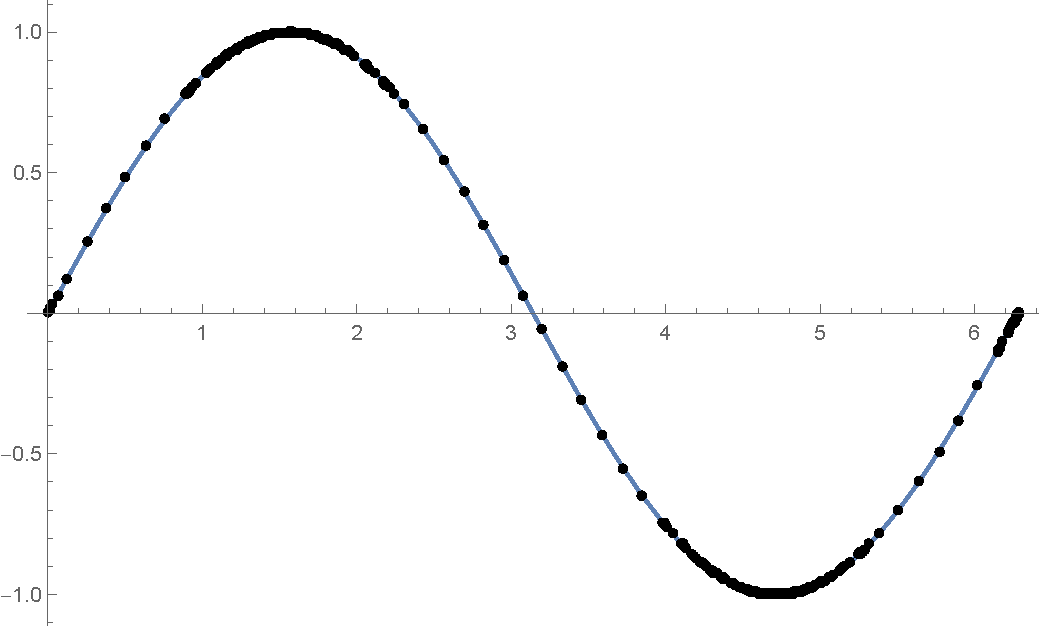
\includegraphics[width=0.5\textwidth]{fig_behaviour_28}
	\caption{A graph of $y=\sin(x)$ generated by Mathematica.}
	\label{fig_behaviour_28}
	\end{center}
\end{figure}

How does Mathematica know where the graph is curvy? Calculus. When we study curvature in a later chapter, we will see how the first and second derivatives of a function work together to provide a measurement of curviness. Mathematica employs algorithms to determine regions of high curvature and plots extra points there.
\fi
\ifpython
Now why are computer graphics so good at curve sketching? It is not because computers are smarter than we are. Rather, it is largely because computers are much faster at computing than we are. In general, computers graph functions plot equally spaced points, then connect the dots using lines. By using lots of points, the connecting lines are short and the graph looks smooth. This does a fine job of graphing in most cases. However, in regions where the graph is very curvy, this can generate noticeable sharp edges on the graph unless a large number of points are used. High quality computer algebra systems, such as Python, use special algorithms to plot lots of points only where the graph is curvy.

In Figure \ref{fig_behaviour_28}, a graph of $y=\sin(x)$ is given, generated by Python using the Python-function \lstinline{Plot}. The small points represent each of the places Python sampled the function. Notice how at the bends of $\sin (x)$, lots of points are used; where $\sin(x)$ is relatively straight, fewer points are used. Moreover, many points are also used at the endpoints to ensure the end behavior is accurate. 
\begin{figure}
	\begin{center}
			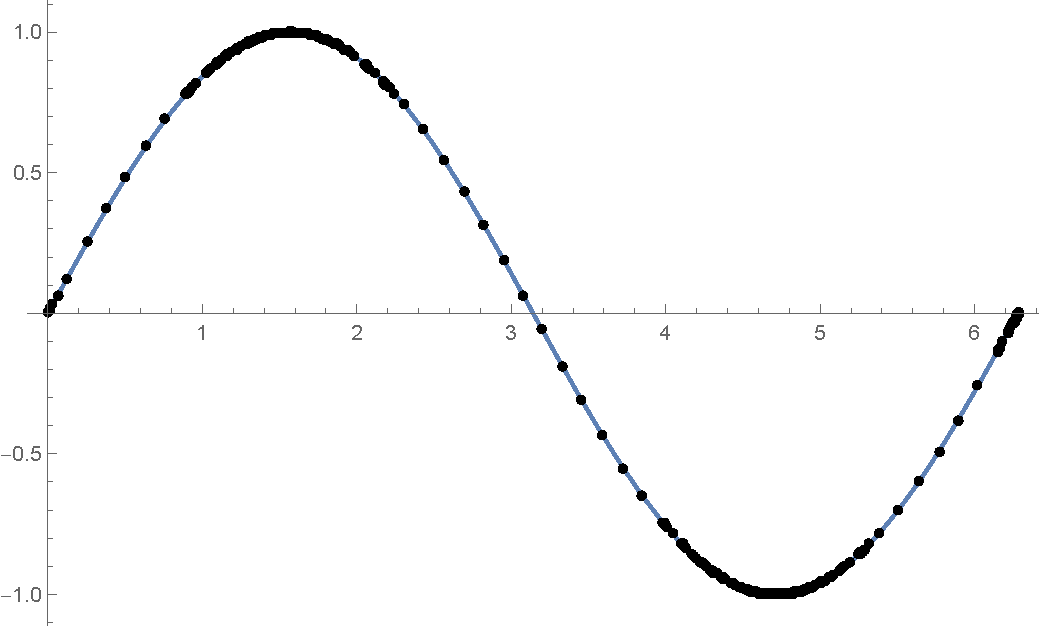
\includegraphics[width=0.5\textwidth]{fig_behaviour_28}
	\caption{A graph of $y=\sin(x)$ generated by Python.}
	\label{fig_behaviour_28}
	\end{center}
\end{figure}
How does Python know where the graph is curvy? Calculus. When we study curvature in a later chapter, we will see how the first and second derivatives of a function work together to provide a measurement of curviness. Python employs algorithms to determine regions of high curvature and plots extra points there.
\fi
Again, the goal of this section is to understand that the shape of the graph of a function is largely determined by understanding the behaviour of the function at a few key places. For instance, in Example \ref{ex_sketch2}, we were able to accurately sketch a complicated graph using only a few points and knowledge of asymptotes!

\begin{remark}[Computer algebra systems]
 A computer algebra system is any mathematical software with the ability to manipulate mathematical expressions in a way similar to the traditional manual computations of mathematicians and scientists. The development of such  systems started in the second half of the previous century. 
 
 The first popular computer algebra systems were muMATH, Reduce, Derive, and Macsyma. Today, the most popular commercial systems are Mathematica and Maple, which are commonly used by research mathematicians, scientists, and engineers. Freely available alternatives include SageMath\footnote{http://www.sagemath.org/} and SymPy. 
\end{remark}

\ifcalculus
\section{Optimization}\label{sec:optimization}

In Section \ref{sec:extreme_values} we learned about extreme values -- the largest and smallest values a function attains on an interval. We motivated our interest in such values by discussing how it made sense to want to know the highest/lowest values of a stock, or the fastest/slowest an object was moving. Here, we apply the concepts of extreme values to solve  problems stated in terms of situations that require us to create the appropriate mathematical framework in which to solve the problem.


We start with a classic example which is followed by a discussion of the topic of optimization.

\begin{example}
\label{ex_opt1}
A man has 100 meters of fencing, a large yard, and a small dog. He wants to create a rectangular enclosure for his dog with the fencing that provides the maximal area. What dimensions provide the maximal area?

\xhrulefill{gray}{2.5pt}Solution \xhrulefill{gray}{2.5pt}

Drawing a rectangle forces us to realize that we need to know the dimensions of this rectangle so we can create an area function -- after all, we are trying to maximize the area. We let $x$ and $y$ denote the lengths of the sides of the rectangle. Clearly, $\text{Area}=xy.$

 We know more about the situation: the man has 100 metres of fencing. By knowing the perimeter of the rectangle must be 100, we can create another equation: $$\text{Perimeter} = 100 = 2x+2y.$$

We now have 2 equations and 2 unknowns. In the latter equation, we solve for $y$:
$$y = 50-x.$$ Now substitute this expression for $y$ in the area equation:
$$ \text{Area} = A(x) = x(50-x).$$ Note we now have an equation of one variable; we can truly call the Area a function of $x$. 

This function only makes sense when $0\leq x \leq 50$, otherwise we get negative values of area. So we find the extreme values of $A(x)$ on the interval $[0,50]$. 

To find the critical points, we take the derivative of $A(x)$ and set it equal to 0, then solve for $x$.
\begin{align*}
A(x) &= x(50-x) \\
			&= 50x-x^2 \\
A'(x) 	&= 50-2x
\end{align*}
We solve $50-2x=0$ to find $x=25$; this is the only critical point. We evaluate $A(x)$ at the endpoints of our interval and at this critical point to find the extreme values; in this case, all we care about is the maximum.

Clearly $A(0)=0$ and $A(50)=0$, whereas $A(25) = 625 \text{m}^2$. This is the maximum. Since we earlier found $y = 50-x$, we find that $y$ is also $25$. Thus the dimensions of the rectangular enclosure with perimeter of 100 m. with maximum area is a square, with sides of length 25 m.
\end{example}

This example is very simplistic and a bit contrived. (After all, most people create a design then buy fencing to meet their needs, and not buy fencing and plan later.) But it models well the necessary process: create equations that describe a situation, reduce an equation to a single variable, then find the needed extreme value.

``In real life,'' problems are much more complex. The equations are often \textit{not} reducible to a single variable (hence multi--variable calculus is needed) and the equations themselves may be difficult to form. Understanding the principles here will provide a good foundation for the mathematics you will likely encounter later.

We outline here the basic process of solving these optimization problems.
\begin{enumerate}
		\item		Understand the problem. Clearly identify what quantity is to be maximized or minimized. Make a sketch if helpful.
		\item		Create equations relevant to the context of the problem, using the information given. 
		\item		If the fundamental equation defines the quantity to be optimized as a function of more than one variable, reduce it to a single variable function using substitutions derived from the other equations.
		\item		Identify the domain of this function, keeping in mind the context of the problem.
		\item		Find the extreme values of this function on the determined domain.
		\item		Identify the values of all relevant quantities of the problem.
		\end{enumerate}


We will now follow these steps in the next example.

\begin{example}
\label{ex_opt2}
Here is another classic calculus problem: A woman has a 100 m of fencing, a small dog, and a large yard that contains a stream (that is mostly straight). She wants to create a rectangular enclosure with maximal area that uses the stream as one side.  What dimensions provide the maximal area?

\xhrulefill{gray}{2.5pt}Solution \xhrulefill{gray}{2.5pt}


We will follow the steps outlined earlier. 
	\begin{enumerate}
	\item		We are maximizing \textit{area}. A sketch of the region will help; Figure \ref{fig_behaviour_29} gives two sketches of the proposed enclosed area. A key feature of the sketches is to acknowledge that one side is not fenced. 

\begin{figure}[H]
	\begin{center}
			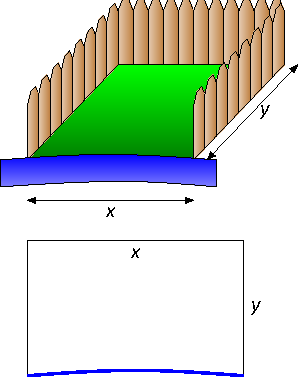
\includegraphics[width=0.5\textwidth]{fig_behaviour_29}
	\caption{A sketch of the enclosure in Example \ref{ex_opt2}.}
	\label{fig_behaviour_29}
	\end{center}
\end{figure}



	
	\item		We want to maximize the area. As in Example~\ref{ex_opt1}, we need another equation to  reduce it to one variable. 
	
	We again appeal to the perimeter; here the perimeter is $$\text{Perimeter} = 100 = x+2y.$$ Note how this is different than in our previous example.
	\item		We now reduce the fundamental equation to a single variable. In the perimeter equation, solve for $y$: $y = 50 - x/2$. We can now write Area as $$\text{Area} = A(x) = x(50-x/2) = 50x - \frac12x^2.$$ Area is now defined as a function of one variable.
	\item		We want the area to be nonnegative. Since $A(x) = x(50-x/2)$, we want $x\geq 0$ and $50-x/2\geq 0$. The latter inequality implies that $x\leq100$, so $0\leq x\leq 100$. 
	\item		We now find the extreme values. At the endpoints, the minimum is found, giving an area of 0. 
	
	Find the critical points. We have $A'(x) = 50-x$; setting this equal to 0 and solving for $x$ returns $x=50$. This gives an area of $$A(50) = 50(25) = 1250.$$
	\item		We earlier set $y = 50-x/2$; thus $y = 25$. Thus our rectangle will have two sides of length 25 and one side of length 50, with a total area of 1250 m$^2$.
	\end{enumerate}
\end{example}

Keep in mind as we do these problems that we are practicing a process; that is, we are learning to turn a situation into a system of equations. These equations allow us to write a certain quantity as a function of one variable, which we then optimize.


Example \ref{ex_opt3} is another classic calculus example, where we focus on minimizing costs.  

\begin{example}
\label{ex_opt3}
A power line needs to be run from a power station located on the beach to an offshore facility. Figure \ref{fig_behaviour_30} shows the distances between the power station to the facility.

It costs \euro50/m. to run a power line along the land, and \euro130/m. to run a power line under water. How much of the power line should be run along the land to minimize the overall cost? What is the minimal cost?

\begin{figure}[H]
	\begin{center}
			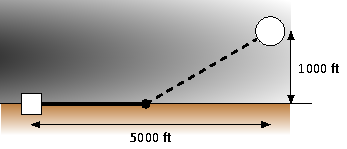
\includegraphics[width=0.5\textwidth]{fig_behaviour_30}
	\caption{Running a power line from the power station to an offshore facility with minimal cost in Example \ref{ex_opt3}.}
	\label{fig_behaviour_30}
	\end{center}
\end{figure}

\xhrulefill{gray}{2.5pt}Solution \xhrulefill{gray}{2.5pt}


There are two immediate solutions that we could consider, each of which we will reject through common sense. First, we could minimize the distance by directly connecting the two locations with a straight line. However, this requires that all the wire be laid underwater, the most costly option. Second, we could minimize the underwater length by running a wire all 5000 m. along the beach, directly across from the offshore facility. This has the undesired effect of having the longest distance of all, probably ensuring a non--minimal cost.

The optimal solution likely has the line being run along the ground for a while, then underwater, as the figure implies. We need to label our unknown distances -- the distance run along the ground and the distance run underwater. Recognizing that the underwater distance can be measured as the hypotenuse of a right triangle, we choose to label the distance run along the ground as $5000-x$, so that the hypotenuse of the right triangle becomes $\sqrt{x^2+1000^2}$. We now create the cost function. 

$$
\begin{array}{ccccc}
\text{Cost} &=&  \text{land cost} &+ & \text{water cost} \\
						&	& \text{\euro50}\times \text{land distance} &+& \text{\euro130}\times \text{water distance} \\
						&	& 50(5000-x) &+& 130\sqrt{x^2+1000^2}.\\
\end{array}
$$

So we have $c(x) = 50(5000-x)+ 130\sqrt{x^2+1000^2}$. This function only makes sense on the interval $[0,5000]$. While we are fairly certain the endpoints will not give a minimal cost, we still evaluate $c(x)$ at each to verify.
$$c(0) = 380,000 \quad\quad c(5000) \approx 662,873.$$

We now find the critical values of $c(x)$. We compute $c'(x)$ as 
$$c'(x) = -50+\frac{130x}{\sqrt{x^2+1000^2}}.$$

Recognize that this is never undefined. Setting $c'(x)=0$ and solving for $x$, we ultimate find that $x=1250/3\approx 416.67$.
Evaluating $c(x)$ at $x=416.67$ gives a cost of about \euro370,000. The distance the power line is laid along land is $5000-416.67 = 4583.33$ m., and the underwater distance is $\sqrt{416.67^2+1000^2} \approx 1083$ m.
\end{example}

In the exercises you will see a variety of situations that require you to combine problem--solving skills with calculus. Focus on  learning how to form equations from situations that can be manipulated into what you need. Eschew memorizing how to do this kind of problem as opposed to that kind of problem. Learning a process will benefit one far longer than memorizing a specific technique.

\fi

In the next chapters, we will consider the reverse problem to computing the derivative: given a function $f$, can we find a function whose derivative is $f$? Being able to do so opens up an incredible world of mathematics and applications.

%%%%%%%%%%%%%%%%%%%%%%%%%%%%%%%%%%%%%%%%%%%%%%%%%%%

\newpage
\section{Exercises}

\renewcommand{\ExerciseListName}{Assignement}

\subsection*{\nameref{sec:extreme_values}}

%%%%%%%%%%%%%%%%%
%Oefening 6 
%%%%%%%%%%%%%%%
\begin{Exercise}[difficulty = 2] Find the extremum of the function $y = x^{(x^2)}$. Prove that it is a minimum.

\end{Exercise}
\setboolean{firstanswerofthechapter}{true}
\begin{Answer}\phantom{}
    $f'(x) = x^{(x^2)} x(2 \ln(x) + 1) = 0 \quad \Leftrightarrow \quad x = e^{-1/2}$ \\[0.2cm]
	$f''(x) = x^{(x^2)} x^2 (2 \ln(x) + 1)^2 + x^{(x^2)} (2 \ln(x) + 3) \quad \Rightarrow \; f''\left( e^{-1/2} \right) = 2 \left( e^{-1/2} \right)^{e^{-1}} >0 $ \\[0.2cm]
	$\Rightarrow \; x = e^{-1/2}$ is a minimum
\end{Answer}
\setboolean{firstanswerofthechapter}{false}
%%%%%%%%%%%%%%%%%
%Oefening 10 Bio-irs
%oefening 12 ings
%%%%%%%%%%%%%%%
\begin{Exercise}[difficulty = 2] The Maxwell-Bolzmann distribution describes the distribution of velocities of gas molecules in an ideal gas. The probability that a molecule with mass $m$ in a gas at temperature $T$, has velocity $v$ is
\[ f(v) = 4\pi\left(\dfrac{m}{2\pi kT}\right)^{3/2}\,v^2\,e^{-\frac{mv^2}{2kT}}, \]
with $k$ a constant. Determine the velocity $v$ for which $f(v)$ is maximal.

\end{Exercise}

\begin{Answer}\phantom{}
$f'(v) = \dfrac{\sqrt{2/\pi}\ m^{3/2}\ v \ e^{-mv^2/(2kT)} \left(2kT-mv^2\right)}{\left(kT\right)^{5/2}}$. \  $f(v)$ is at a maximum if $v=\sqrt{\dfrac{2kT}{m}}$.
\end{Answer}

\subsection*{\nameref{sec:mvt}}
%%%%%%%%%%%%%%%%%
%Oefening 3
%%%%%%%%%%%%%%%
\begin{Exercise} For the functions listed below, verify whether the mean value theorem (theorem~\ref{thm:mvt}) can be applied to the given interval. Determine, if possible, a $c \in [a,b]$ that is guaranteed by the theorem. 
    \Question[difficulty = 2] $f(x) = x^2+3x-1, \qquad [-2,2] $
    \Question[difficulty = 2] $f(x) = \sqrt{9-x^2}, \qquad [0,3] $ 
    \Question[difficulty = 2] $f(x) = \dfrac{x^2-9}{x^2-1}, \qquad [0,2] $ 
    
\end{Exercise}

\begin{Answer}\phantom{}
    \Question $c=0$ 
    \Question $c=3/\sqrt{2}$ 
    \Question The mean value theorem is not applicable.
   
\end{Answer}

%%%%%%%%%%%%%%%%%
%Oefening 4
%%%%%%%%%%%%%%%
\begin{Exercise} For the functions listed below, verify that Rolle's theorem (stelling~\ref{thm:rolles}) can be applied to the given interval. Determine, if possible, a $c \in [a,b]$ such that $f'(c)=0$. 
    \ifanalysis\Question[difficulty = 1]\fi \ifcalculus\Question[difficulty = 2]\fi $f(x) = x^2+x-6, \qquad [-3,2] $
    \ifanalysis\Question[difficulty = 1]\fi\ifcalculus\Question[difficulty = 2]\fi $f(x) = x^2+x, \qquad [-2,2] $ 
    \ifanalysis\Question[difficulty = 1]\fi\ifcalculus\Question[difficulty = 2]\fi $f(x) = \cos (x), \qquad [0,\pi] $ 

\end{Exercise}

\begin{Answer}\phantom{}
        \Question $c=-1/2$ 
        \Question Rolle's theorem is not applicable.
        \Question Rolle's theorem is not applicable.
\end{Answer}


\subsection*{\nameref{sec:sketch}}


\ifanalysis
%%%%%%%%%%%%%%%%%
%Oefening 8 Bio-irs
%%%%%%%%%%%%%%%

\begin{Exercise}[difficulty = 2] %Oude examenvraag Bio-ir
\
    \Question Examine the graph of the function $y=x e^{-kx^2}$, with $k \in \mathbb{R}$. To do this, determine its domain, zeros, symmetries, asymptotes, extrema and inflection points. When determining the asymptotes, discuss the different values of $k$ ($k<0$, $k=0$, $k>0$).
    
    \Question Determine the value of the parameter $k$ such that a maximum occurs at $x=1$.
    
    \Question Make a sign table of the function and a sketch of the graph for the value of $k$.

\end{Exercise}

\begin{Answer}\phantom{}
    
        \Question The function with parameter $k>0$ has a horizontal asymptote $y=0$ for $x \rightarrow \pm \infty$. \\
        Derivatives: $\quad f'(x)=e^{-kx^2} \left( 1 - 2x^2k \right)\qquad\mbox{en}\qquad f''(x)=-2kxe^{-kx^2} \left( 3 - 2x^2k \right)$
        
        \Question $k=\dfrac{1}{2}$
        
        \Question 
       Summary for: $f(x) = x e^{-\frac{x^2}{2}}$
        \[ \begin{array}{r|ccccccccccccc}
    		x & -\infty & & - \sqrt{3} &  & -1 &  & 0 &  & 1 & &\sqrt{3} &  &+\infty \\
    		\hline
    		f'(x)   & - & - & - & - & 0 & + & + & + & 0 & - & - & - & - \\
    		f''(x)  & - & - & 0 & + & + & + & 0 & - & - & - & 0 & + & + \\
    		\hline
    		&&&&&&&&&\vspace{-0.3cm}\\
    		f(x)    & (0) & \searrow  & f(-\sqrt{3}) &  \searrow & f(-1) & \nearrow & 0 & \nearrow & f(1) & \searrow & f(\sqrt{3}) & \searrow & (0)\\
    		&&&&&&&&&\vspace{-0.3cm}\\                                                                              
    		& \mbox{H.A.} & \cap & \mbox{inf.p.} & \cup & \mbox{min.} & \cup & \mbox{inf.p.} & \cap &  \mbox{max.} & \cap & \mbox{inf.p.} & \cup & \mbox{H.A.} \\
    		\end{array}\]
   
\end{Answer}
\fi

%%%%%%%%%%%%%%%%%
%Oefening 9 Bio-irs
%Oefening 7 Ings
%%%%%%%%%%%%%%%



\begin{Exercise} Sketch the graph of the following functions.
\begin{multicols}{2}
    \ifcalculus \Question[difficulty = 1] $f(x)=\sqrt{x^2-1}$ \fi
	\Question[difficulty = 1] $f(x)=\sqrt{x^2-4x+3}$ 
	\ifcalculus \Question[difficulty = 1] $f(x) = \dfrac{x^3}{3-x^2}$ \fi %uit Van Hecke H7, vb 7.4
	\ifanalysis\Question[difficulty = 1]\fi\ifcalculus\Question[difficulty = 2]\fi $f(x)=\dfrac{x+7}{\sqrt{x^2-3}}$ 
	\Question[difficulty = 1] $f(x)=e^{-\frac{x^2}{2}}$
	\ifcalculus \Question[difficulty = 2] $f(x)=x^3\,e^{-x}$ \fi
	\ifanalysis\Question[difficulty = 1]\fi\ifcalculus\Question[difficulty = 2]\fi $f(x)=\dfrac{e^{-x}}{x^3}$  
	\Question[difficulty = 1] $f(x)=\ln (2^x-1)$
	\ifanalysis\Question[difficulty = 1]\fi\ifcalculus\Question[difficulty = 2]\fi $f(x)=\dfrac{\ln (x)}{x^2}$ 
	\Question[difficulty = 2] $f(x)=\ln\left(\sqrt{e^x+e^{-x}}\right)$
	\ifanalysis\Question[difficulty = 1]\fi\ifcalculus\Question[difficulty = 2]\fi $f(x)=\dfrac{2\ln (x)}{1- \ln (x)}$
	\Question[difficulty = 1] $f(x)=\ln\left( \cos (x)\right)$ 
	\Question[difficulty = 2] $f(x)=\arctan(\ln (x))$ 
	\Question[difficulty = 1] $f(x)=\arctan \left(\dfrac{1}{x}\right)$ 
	\Question[difficulty = 2] $f(x)=x^x$ 
	\Question[difficulty = 2] $f(x)=(x^2)^x$  
	%\Question [] Tip: $f''(x)=(x^2)^x\left(\left(\ln (x^2)+2\right)^2+\dfrac{2}{x}\right)$
	\Question[difficulty = 1] $f(x) = x - 2\sin(x)$ 
	\Question[difficulty = 2] $f(x) = e^{-x} \sin(x), \quad (x \geq 0)$ 
	\Question[difficulty = 1] $f(x) = x + \sin(x)$ 
	\ifanalysis\Question[difficulty = 1]\fi\ifcalculus\Question[difficulty = 2]\fi $f(x)= \dfrac{|1+x|-1}{x}$ 
	\ifanalysis\Question[difficulty = 1]\fi\ifcalculus\Question[difficulty = 2]\fi $f(x) = \left|  2- \sqrt{2x+4} \right|$ 
	\ifanalysis\Question[difficulty = 1]\fi\ifcalculus\Question[difficulty = 2]\fi $f(x) = \dfrac{x^2}{x|x| + 1}$
	\ifanalysis\Question[difficulty = 1]\fi\ifcalculus\Question[difficulty = 2]\fi $f(x) = \left| (x-2)^2-4 \right| $
	\ifanalysis
	 \Question[difficulty = 1] $f(x)=\sinh (x)-x$
     \Question[difficulty = 1] $f(x)=e^x \sinh (x)$
     \Question[difficulty = 1] $f(x)=\coth (x) + x$
     \Question[difficulty = 2] $f(x)=\arcosh (\sqrt{x-2})$
     \Question[difficulty = 1] $f(x)=\artanh \left( \dfrac{4}{x} \right)$
	\fi
    \EndCurrentQuestion
\end{multicols}

\end{Exercise}

\begin{Answer}\phantom{}
    
	    \ifcalculus 	
    	\Question Asymptotes: $\quad y=x \quad$ and $\quad y=-x$\par
    		Derivatives: $\quad f'(x)=\dfrac{x}{\sqrt{x^2-1}}\qquad\mbox{en}\qquad f''(x)=-\dfrac{1}{(x^2-1)^\frac{3}{2}}$
    		\[ \begin{array}{r|ccccccc}
    		x & -\infty  &  & -1 &  & 1 & &+\infty \\
    		\hline
    		f'(x)   & - & - & | & /// & | & + & + \\
    		f''(x)  & - & - & | & /// & | & - & - \\
    		\hline
    		&&&&&&&\vspace{-0.3cm}\\
    		f(x)    & (+\infty) & \searrow & 0 & ///& 0 & \nearrow & (+\infty)\\
    		&&&&&&&\vspace{-0.3cm}\\                                                                              
    		& & \cap & & &  & \cap &  \\
    		\end{array}\]
    	\fi
    
    	\Question Asymptotes: $\quad y=x-2\quad$ and $\quad y=-x+2$\par
    		Derivatives: $\quad f'(x)=\dfrac{x-2}{\sqrt{x^2-4x+3}}\qquad\mbox{and}\qquad f''(x)=-\dfrac{1}{(x^2-4x+3)^\frac{3}{2}}$
    		\[ \begin{array}{r|ccccccc}
    		x & -\infty  &  & 1 &  & 3 & &+\infty \\
    		\hline
    		f'(x)   & - & - & | & /// & | & + & + \\
    		f''(x)  & - & - & | & /// & | & - & - \\
    		\hline
    		&&&&&&&\vspace{-0.3cm}\\
    		f(x)    & (+\infty) & \searrow & 0 & ///& 0 & \nearrow & (+\infty)\\
    		&&&&&&&\vspace{-0.3cm}\\                                                                              
    		& \mbox{S.A.} & \cap & & &  & \cap & \mbox{S.A.} \\
    		\end{array}\]
    		
    	\ifcalculus 
    	\Question Asymptotes: $\quad x=-\sqrt{3},\quad x=\sqrt{3},\quad y=-x$\par
    		Derivatives: $\quad f'(x)=\dfrac{x^2(9-x^2)}{(3-x^2)^2}\qquad\mbox{and}\qquad f''(x)=\dfrac{6x(9+x^2)}{(3-x^2)^3}$
    		\[ \begin{array}{r|ccccccccccccc}
    		x & -\infty  &  & -3 &  & -\sqrt{3}  & &  0 & &  \sqrt{3} & & 3 & & +\infty \\
    		\hline
    		f'(x)   & - & - & 0 & + & | & + & 0 & + & | & + & 0 & - & -  \\
    		f''(x)  & + & + &  & + & | & - & 0 & + & | & -  &  & - & -  \\
    		\hline
    		&&&&&&&&&&&&&\vspace{-0.3cm}\\
    		f(x)  &  (+\infty) & \searrow & 9/2 & \nearrow & | & \nearrow & 0 & \nearrow   & | & \nearrow & -9/2 & \searrow &  (-\infty) \\
    		&&&&&&&&&&&&&
    		\vspace{-0.3cm}\\                             
    		& \mbox{S.A.} & \cup   &   & \cup & \mbox{V.A.} & \cap & &\cup & \mbox{V.A.} & \cap & & \cap & \mbox{S.A.} \\
    		\end{array}\]
    	\fi	
    	
    	\Question Asymptotes: $\quad x=-\sqrt{3},\quad x=\sqrt{3},\quad y=-1\quad$ and $\quad y=1$\par
    		Derivatives: $\quad f'(x)=-\dfrac{7x+3}{(x^2-3)^{\frac{3}{2}}}\qquad\mbox{and}\qquad f''(x)=\dfrac{14x^2+9x+21}{(x^2-3)^{\frac{5}{2}}}$
    		\[ \begin{array}{r|ccccccccc}
    		x & -\infty  &  & -7 &  & -\sqrt{3} & & \sqrt{3} & &+\infty \\
    		\hline
    		f'(x)   & + & + & + & + & | & /// & | & - & -\\
    		f''(x)  & + & + & + & + & | & /// & | & + & +\\
    		\hline
    		&&&&&&&&&\vspace{-0.3cm}\\
    		f(x)    & (-1) & \nearrow & 0 & \nearrow & | & /// & | & \searrow & (1)\\
    		&&&&&&&&&\vspace{-0.3cm}\\                                                                              
    		& \mbox{H.A.} & \cup   & \cup & \cup & \mbox{V.A.} &  & \mbox{V.A.} & \cup & \mbox{H.A.} \\
    		\end{array}\]
    		
    	
    	\Question Asymptotes: $\quad y=0$\par
    		Derivatives: $\quad f'(x)=-x e^{-\frac{x^2}{2}}\qquad\mbox{and}\qquad f''(x)=\left(x^2-1\right)e^{-\frac{x^2}{2}}$
    		\[ \begin{array}{r|ccccccccc}
    		x & -\infty & & -1 &  & 0 &  & 1 & &+\infty \\
    		\hline
    		f'(x)   & + & + & + & + & 0 & - & - & - & - \\
    		f''(x)  & + & + & 0 & - & - & - & 0 & + & + \\
    		\hline
    		&&&&&&&&&\vspace{-0.3cm}\\
    		f(x)    & (0) & \nearrow & \nearrow & \nearrow & 1 & \searrow & \searrow & \searrow & (0)\\
    		&&&&&&&&&\vspace{-0.3cm}\\                                                                              
    		& \mbox{H.A.} & \cup & \mbox{inf.p.} & \cap & \mbox{max.} & \cap & \mbox{inf.p.} & \cup & \mbox{H.A.} \\
    		\end{array}\]
    		
    		\ifcalculus 
    		\Question Asymptotes: $\quad y=0$\par
    		Derivatives: $\quad f'(x)=e^{-x}\left(-x^3+3x^2\right)\qquad\mbox{and}\qquad f''(x)=e^{-x}\left(x^3-6x^2+6x\right)$
    		\[ \begin{array}{r|ccccccccccc}
    		x & -\infty & & 0 & & 3-\sqrt{3} &  & 3 & & 3+\sqrt{3} &  &+\infty \\
    		\hline
    		f'(x) & +  & + & 0 & + & + & + & 0 & - & - & - & - \\
    		f''(x) & -  & - & 0 & + & 0 & - & - & - & 0 & + & + \\
    		\hline
    		&&&&&&&&&&&\vspace{-0.3cm}\\
    		f(x)    & (-\infty) & \nearrow & 0 & \nearrow & (3-\sqrt{3})e^{-3+\sqrt{3}} & \nearrow & 27e^{-3} & \searrow & (3+\sqrt{3})e^{-3-\sqrt{3}} & \searrow & (0)\\
    		&&&&&&&&&&&\vspace{-0.3cm}\\                                                                              
    		&  & \cap & \mbox{inf.p.} & \cup & \mbox{inf.p.} & \cap  & \mbox{max.} & \cap &  \mbox{inf.p.} & \cup & \mbox{H.A.} \\
    		\end{array}\]
    		\fi
    		
    
    	\Question Asymptotes: $\quad x=0\quad\mbox{and}\quad y=0$\par
    		Derivatives: $\quad f'(x)=-\dfrac{e^{-x}(x+3)}{x^4}\qquad\mbox{and}\qquad f''(x)=\dfrac{e^{-x}\left(x^2+6x+12\right)}{x^5}$
    		\[ \begin{array}{r|ccccccc}
    		x & -\infty & & -3 &  & 0 &  &+\infty \\
    		\hline
    		f'(x)   & + & + & 0 & - & | & - & - \\
    		f''(x)  & - & - & - & - & | & + & + \\
    		\hline
    		&&&&&&&\vspace{-0.3cm}\\
    		f(x)    & (-\infty) & \nearrow & -\dfrac{e^3}{27} & \searrow & | & \searrow & (0)\\
    		&&&&&&&\vspace{-0.3cm}\\                                                                              
    		&  & \cap & \mbox{max.} & \cap & \mbox{V.A.} & \cup & \mbox{H.A.} \\
    		\end{array}\]
    		
    	\Question Asymptotes: \quad $x=0\quad\mbox{and}\quad y=\ln (2) x$\par
    		Derivatives: $\quad f'(x)=\dfrac{2^x\ln (2)}{2^x-1}\qquad\mbox{and}\qquad f''(x)=-\dfrac{2^x\ln^2(2)}{(2^x-1)^2}$
    		\[ \begin{array}{r|cccccc}
    		x &  & 0 &  & 1 & &+\infty \\
    		\hline
    		f'(x)   & /// & | & + & + & + & + \\
    		f''(x)  & /// & | & - & - & - & - \\
    		\hline
    		&&&&&&\vspace{-0.3cm}\\
    		f(x)    & /// & | & \nearrow & 0 & \nearrow & (+\infty)\\
    		&&&&&&\vspace{-0.3cm}\\                                                                              
    		& & \mbox{V.A.} & \cap & \cap & \cap & \mbox{S.A.} \\
    		\end{array}\]
    		
    	\Question Asymptotes: \quad $x=0\quad\mbox{and}\quad y=0$\par
    		Derivatives: $\quad f'(x)=\dfrac{1-2\ln (x)}{x^3}\qquad\mbox{and}\qquad f''(x)=\dfrac{6\ln (x)-5}{x^4}$
    		\[ \begin{array}{r|cccccccccc}
    		x &  & 0 & & 1 &  & \sqrt{e} &  & e^\frac{5}{6} & & +\infty \\
    		\hline
    		f'(x)   & /// & | & + & + & + & 0 &  - & - & - & - \\
    		f''(x)  & /// & | & - & - & - & - & - & 0 & + & + \\
    		\hline
    		&&&&&&&&&&\vspace{-0.3cm}\\
    		f(x)    & /// & | & \nearrow & \nearrow & \nearrow & \dfrac{1}{2e} & \searrow & \searrow & \searrow & (0)\\
    		&&&&&&&&\vspace{-0.3cm}\\                                                                              
    		& & \mbox{V.A.} & \cap & \cap & \cap & \mbox{max.} & \cap & \mbox{inf.p.} & \cup & \mbox{H.A.} \\
    		\end{array}\]
    		
    
    	\Question Asymptotes: \quad $y=\dfrac{x}{2}\quad\mbox{and}\quad y=-\dfrac{x}{2}$\par
    		Derivatives: $\quad f'(x)=\dfrac{e^{x}-e^{-x}}{2(e^{x}+e^{-x})}\qquad\mbox{and}\qquad f''(x)=\dfrac{2}{(e^{x}+e^{-x})^2}$
    		\[ \begin{array}{r|ccccc}
    		x &  -\infty &  & 0 & &+\infty \\
    		\hline
    		f'(x)   &  - & - & 0 & + & + \\
    		f''(x)  &  + & + & + & + & + \\
    		\hline
    		&&&&&\vspace{-0.3cm}\\
    		f(x)    &  (+\infty) & \searrow & \dfrac{\ln (2)}{2} & \nearrow & (+\infty)\\
    		&&&&&\vspace{-0.3cm}\\                                                                              
    		& \mbox{S.A.} & \cup & \mbox{min.} & \cup & \mbox{S.A.} \\
    		\end{array}\]
    		
    
    	\Question Asymptotes: \quad $x=e\quad\mbox{and}\quad y=-2$\par
    		Derivatives: $\quad f'(x)=\dfrac{2}{(\ln (x)-1)^2\, x}\qquad\mbox{and}\qquad f''(x)=-\dfrac{2(\ln (x)+1)}{(\ln (x)-1)^3\, x^2}$
    		\[ \begin{array}{r|cccccccc}
    		x &  & 0 &  & e^{-1} &  & e & &+\infty \\
    		\hline
    		f'(x)   & /// & | & + & + & + & | & + & + \\
    		f''(x)  & /// & | & - & 0 & + & | & - & - \\
    		\hline
    		&&&&&&&&\vspace{-0.3cm}\\
    		f(x)    & /// & (-2) & \nearrow & \nearrow & \nearrow & | & \nearrow & (-2)\\
    		&&&&&&&&\vspace{-0.3cm}\\                                                                              
    		& & & \cap & \mbox{inf.p.} & \cup & \mbox{V.A.} & \cap & \mbox{H.A.}  \\
    		\end{array}\]
    		
    
    	\Question Asymptotes: \quad $x=\dfrac{\pi}{2}+k\pi,\, k\in\mathbb{Z}$\par
    		Derivatives: $\quad f'(x)=-\tan (x)\qquad\mbox{and}\qquad f''(x)=-\dfrac{1}{\cos^2 (x)}$
    		\begin{footnotesize}\[ \begin{array}{r|ccccccccccccccc}
    			x  & \cdots & & -\dfrac{\pi}{2} &  & 0 &  & \dfrac{\pi}{2} & & \dfrac{3\pi}{2} & & 2\pi & & \dfrac{5\pi}{2} & & \cdots  \\[0.2cm]
    			\hline
    			f'(x)    & \cdots & /// & | & + & 0 & - & | & /// & | & + & 0 & - & | & /// & \cdots  \\
    			f''(x)   & \cdots & /// & | & - & - & - & | & /// & | & - & - & - & | & /// & \cdots  \\
    			\hline
    			&&&&&&&&&&&&&&\vspace{-0.3cm}\\
    			f(x)     & \cdots & /// & | & \nearrow & \mbox{max.} & \searrow & | & /// & | & \nearrow & \mbox{max.} & \searrow & | & /// & \cdots \\
    			&&&&&&&&&&&&&&\vspace{-0.3cm}\\                                                                              
    			&  &  & \mbox{V.A.}  & \cap & \cap & \cap & \mbox{V.A.} &  & \mbox{V.A.} & \cap & \cap & \cap & \mbox{V.A.}  &  &    \\
    			\end{array}\]\end{footnotesize}
    		There are an infinite number of maxima at $x=2k\pi$, with $k\in\mathbb{Z}$.
    		
    
    	\Question Asymptotes: \quad $y=\dfrac{\pi}{2}$\par
    		Derivatives: $\quad f'(x)=\dfrac{1}{x(1+\ln^2(x))}\qquad\mbox{and}\qquad f''(x)=-\dfrac{(1+\ln (x))^2}{x^2(1+\ln^2(x))^2}$
    		\[ \begin{array}{r|cccccccc}
    		x &  & 0 &  & e^{-1} &  & 1 & &+\infty \\
    		\hline
    		f'(x)   & /// & | & + & + & + & + & + & + \\
    		f''(x)  & /// & | & - & 0 & - & - & - & - \\
    		\hline
    		&&&&&&&&\vspace{-0.3cm}\\
    		f(x)    & /// & \left(-\dfrac{\pi}{2}\right) & \nearrow & \nearrow & \nearrow & 0 & \nearrow & \left(\dfrac{\pi}{2}\right)\\
    		&&&&&&&&\vspace{-0.3cm}\\                                                                              
    		& &  & \cap & \cap & \cap & \cap & \cap & \mbox{H.A.} \\
    		\end{array}\]
    		
    
    	\Question Asymptotes: \quad $y=0$\par
    		Derivatives: $\quad f'(x)=-\dfrac{1}{1+x^{2}}\qquad\mbox{and}\qquad f''(x)=\dfrac{2x}{\left(1+x^{2}\right)^2}$
    		\[ \begin{array}{r|ccccc}
    		x &  -\infty &  & 0 & &+\infty \\
    		\hline
    		f'(x)   &  - & - & | & - & - \\
    		f''(x)  &  - & - & | & + & + \\
    		\hline
    		&&&&&\vspace{-0.3cm}\\
    		f(x)    &  (0) & \searrow & \left(-\frac{\pi}{2}\left|\,\frac{\pi}{2} \right.\right) & \searrow & (0)\\
    		&&&&&\vspace{-0.3cm}\\                                                                              
    		& \mbox{H.A.} & \cap & \mbox{V.A.} & \cup & \mbox{H.A.} \\
    		\end{array}\]
    		
    	\Question Asymptotes: \quad none\par
    		Derivatives: $\quad f'(x)=x^x(\ln (x)+1)\qquad\mbox{and}\qquad f''(x)=x^x\left((\ln (x) +1)^2+\dfrac{1}{x}\right)$
    		\[ \begin{array}{r|cccccc}
    		x &  & 0 &  & e^{-1} & &+\infty \\
    		\hline
    		f'(x)   & /// & | & - & 0 & + & + \\
    		f''(x)  & /// & | & + & + & + & + \\
    		\hline
    		&&&&&&\vspace{-0.3cm}\\
    		f(x)    & /// & (1) & \searrow & e^{-e^{-1}} & \nearrow & (+\infty)\\
    		&&&&&&\vspace{-0.3cm}\\                                                                              
    		& &  & \cup & \mbox{min.} & \cup &  \\
    		\end{array}\]
    		
    
    	\Question Asymptotes: \quad $y=0$\par
    		Derivatives: $\quad f'(x)=(x^2)^x(\ln (x^2) + 2)\qquad\mbox{and}\qquad f''(x)=(x^2)^x\left(\left(\ln (x^2)+2\right)^2+\dfrac{2}{x}\right)$
    		\[ \begin{array}{r|ccccccccccc}
    		x & -\infty & & -0,8 &  & -\dfrac{1}{e} & & 0 & & \dfrac{1}{e} & &+\infty \\[0.2cm]
    		\hline
    		f'(x)   & + & + & + & + & 0 & - & | & - & 0 & + & +\\
    		f''(x)  & + & + & 0 & - & - & - & | & + & + & + & +\\
    		\hline
    		&&&&&&&&&&&\vspace{-0.3cm}\\
    		f(x)    & (0) & \nearrow & \nearrow & \nearrow & e^{2e^{-1}} & \searrow & (1) & \searrow & e^{-2e^{-1}} & \nearrow & (+\infty)\\
    		&&&&&&&&&&&\vspace{-0.3cm}\\                                                                              
    		& \mbox{H.A.} & \cup & \mbox{inf.p.} & \cap & \mbox{max.} & \cap & & \cup & \mbox{min.} & \cup & \cup \\
    		\end{array}\]
    		
    	\Question Asymptotes: \quad none\par
                Derivatives: $\quad f'(x)=1-2\cos (x) \qquad\mbox{and}\qquad f''(x)=2\sin (x)$
                   \begin{footnotesize}
                \[ \begin{array}{r|ccccccccccccccc}
                x & \cdots &0 & & \dfrac{\pi}{3} & & \pi & & \dfrac{5\pi}{3} & & 2\pi & & \dfrac{7\pi}{3} & &  3 \pi& \cdots \\[0.2cm]
                \hline
                f'(x) & \cdots  & - & - & 0 & + & + & + & 0 & - & - & - & 0 & + & + & \cdots \\
                f''(x) & \cdots& 0 & + & + & + & 0 & - & - & - & 0 & + & + & + & 0 & \cdots\\
                \hline
                &&&&&\vspace{-0.3cm}\\
                f(x) & (-\infty) & 0 & \searrow & f\left(\dfrac{\pi}{3}\right) & \nearrow & f(\pi) & \nearrow & f\left(\dfrac{5\pi}{3}\right) & \searrow & f(2\pi) & \searrow & f\left(\dfrac{7\pi}{3}\right)& \nearrow &  f(3\pi) & (+\infty)  \\
                &&&&&\vspace{-0.3cm}\\                                                                      
                    & \cdots  & \mbox{inf.p.}& \cup& \mbox{min.} & \cup & \mbox{inf.p.} & \cap & \mbox{max.}& \cap & \mbox{inf.p.}  &\cup& \mbox{min.} & \cup & \mbox{inf.p.} &  \cdots \\
                \end{array}\]
                   \end{footnotesize}
                
        \Question Asymptotes: \quad y=0\par
                  Derivatives: $\quad f'(x)= e^{-x}(- \sin (x) + \cos (x)) \qquad\mbox{and}\qquad f''(x) = -2 e^{-x} \cos (x)$
                   \begin{footnotesize} \[ %\setlength{\arraycolsep}{2pt}
                \begin{array}{r|cccccccccccccccccc}
                x &  0 & & \dfrac{\pi}{4} & & \dfrac{\pi}{2} &  & \pi & & \dfrac{5\pi}{4} & & \dfrac{3\pi}{2} & & 2\pi & & \dfrac{9\pi}{4} & & \dfrac{5\pi}{2}  & \cdots \\[0.2cm]
                \hline
                f'(x) &   + & + & 0 & -&- & -& - &- & 0 & +& + & + & + & + & 0 & -&- & \cdots     \\
                f''(x) & -& - & - & - & 0 &+ & + & +& + & +  & 0 &- & - & - & - & - & 0 & \cdots  \\
                \hline 
                &&&&\vspace{-0.3cm}\\
                f(x) &  0 & \nearrow & f\left(\dfrac{\pi}{4}\right)  & \searrow & f\left(\dfrac{\pi}{2}\right) & \searrow &  0 & \searrow & f\left(\dfrac{5\pi}{4}\right)  & \nearrow & f\left(\dfrac{3\pi}{2}\right) &  \nearrow & 0 &  \nearrow &f\left(\dfrac{9\pi}{4}\right)& \searrow & f\left(\dfrac{5\pi}{2}\right)  & (0)  \\
                
                & & \cap & \mbox{max.} & \cap & \mbox{inf.p.}  & \cup & & \cup & \mbox{min.}  & \cup & \mbox{inf.p.} & \cap & & \cap &   \mbox{max.}   & \cap &  \mbox{inf.p.} & \cdots
                \end{array} \] \end{footnotesize}
    
    
        \Question Asymptotes: \quad none\par
                Derivatives: $\quad f'(x)=1+\cos (x) \qquad\mbox{and}\qquad f''(x)=-\sin (x)$
                \[ \begin{array}{r|ccccccccccccccc}
                x & \cdots & \cdots & -2\pi & & -\pi &  & 0 & & \pi & & 2\pi & & 3\pi &  \cdots & \cdots \\[0.2cm]
                \hline
                f'(x) & \cdots & \cdots & + & +& 0 & + & + & + & 0 & + & + & + & 0 &  \cdots &  \cdots \\
                f''(x) &\cdots & + & 0 & - & 0 & + & 0 & - & 0 & + & 0 & - & 0 &+ &\cdots\\
                \hline
                &&&&&\vspace{-0.3cm}\\
                f(x) & (-\infty) & \nearrow   & f(-2\pi) & \nearrow & f(-\pi) & \nearrow & f(0) & \nearrow & f\left(\pi\right) & \nearrow & f(2\pi) & \nearrow & f\left(3\pi\right)& \nearrow   & (+\infty)  \\
                &&&&&\vspace{-0.3cm}\\                                                                      
                   & \cdots & \cup  & \mbox{inf.p.}  & \cap & \mbox{inf.p.} & \cup & \mbox{inf.p.} & \cap & \mbox{inf.p.}  & \cup & \mbox{inf.p.}  &\cap& \mbox{inf.p.}  & \cup & \cdots  \\
                \end{array}\]
                
        \Question $f(x) = \dfrac{|1+x|-1}{x} = \left\{ \begin{array}{ll} 1, & \quad \text{ if } x \geq -1, \\
    		-\dfrac{x+2}{x} = -1 -\dfrac{2}{x}, & \quad \text{ if } x < -1. \end{array} \right.$ \\[0.2cm]
    		    Asymptotes: $\quad y=-1$ \quad (for $x\rightarrow -\infty$) \\[0.2cm]
    		    Derivatives: $\quad f'(x) = \left\{ \begin{array}{ll} 0, & \quad \text{ if } x \geq -1, \\
    		\dfrac{2}{x^2}, & \quad \text{ if } x < -1. \end{array} \right. \qquad\mbox{and}\qquad \quad f''(x) = \left\{ \begin{array}{ll} 0, & \quad \text{ if } x \geq -1, \\
    		\dfrac{-4}{x^3}, & \quad \text{ if } x < -1. \end{array} \right.$ \\
    		
    		
    		\[ \begin{array}{r|ccccccccc}
            x & -\infty & & -2 & & -1 & & 0 & & +\infty \\[0.1cm]
            \hline
            f'(x)   & + & + & + & + & 2 & 0 & 0 & 0 & 0\\
            f''(x)  & + & + & + & + & 4 & 0 & 0 & 0 & 0\\
            \hline
            &&&&&&&&&\vspace{-0.3cm}\\
            f(x)    & (-1) & \nearrow & 0 & \nearrow & 1 & 1 & (1) & 1 & 1\\
            &&&&&&&&&\vspace{-0.3cm}\\                  
            & \mbox{H.A.} & \cup &  & \cup &  & - &  & - &  \\
            \end{array}\]
    		
    		
    	\Question $f(x) = \left|  2- \sqrt{2x+4} \right| \qquad \Rightarrow \quad \dom\,f(x)=[-2, + \infty[, \qquad f(x)=0 \quad \Leftrightarrow \quad x=0$ \\[0.2cm]
    		$\Rightarrow \; f(x)= \left\{ \begin{array}{ll} 2-\sqrt{2x+4}, & \quad \text{ if } -2 \leq x <0, \\
    		-2+\sqrt{2x+4}, & \quad \text{ if } x > 0. \end{array} \right.$ \\[0.2cm]
    		
    		\begin{itemize}
    		    \item $f(x) = 2-\sqrt{2x+4}$ \quad with $-2 \leq x <0$
    		    \item [] Asymptotes: \quad none \par
                         Derivatives: $\quad f'(x)=-\dfrac{1}{\sqrt{2x+4}} \qquad\mbox{and}\qquad f''(x)=\dfrac{1}{\sqrt{(2x+4)^3}}$
    		    
    		    \item $f(x) = -2+\sqrt{2x+4}$ \quad with $x > 0$
    		    \item [] Asymptotes: \quad none\par
                         Derivatives: $\quad f'(x)=\dfrac{1}{\sqrt{2x+4}} \qquad\mbox{and}\qquad f''(x)=-\dfrac{1}{\sqrt{(2x+4)^3}}$
    		\end{itemize}
    		
    		
    		 \[ \begin{array}{r|ccccccc}
                x &  & -2 &  & 0 & &  & +\infty \\
                \hline
                f'(x)   &  & | &  - &  \left(-\frac{1}{2}\left|\,\frac{1}{2} \right.\right) & + & + & +  \\
                f''(x)  &  & | &  + & \left(\frac{1}{8}\left|\,-\frac{1}{8}\right.\right)  & - & - & - \\
                \hline
                &&&&&\vspace{-0.3cm}\\
                f(x)    &  & 2  & \searrow & 0 & \nearrow & \nearrow & (+\infty) \\
                &&&&&\vspace{-0.3cm}\\                                                                              
                       & & & \cup  & \mbox{inf.p.} & \cap & \cap & \cap \\
                \end{array}\]
    		
    
    	\Question $f(x) = \dfrac{x^2}{x|x| + 1}
    		\qquad \Rightarrow \quad  f(x)=0 \quad \Leftrightarrow \quad x=0$ \\[0.2cm]
    		$\Rightarrow \; f(x)= \left\{ \begin{array}{ll} \dfrac{x^2}{-x^2 + 1}, & \quad \text{ if }  x <0, \\
    		\dfrac{x^2}{x^2 + 1}, & \quad \text{ if } x > 0. \end{array} \right.$ \\[0.2cm]
    		
    		\begin{itemize}
    		    \item $f(x) = \dfrac{x^2}{-x^2 + 1}$ \quad with $x <0$
    		    \item [] Asymptotes: \quad $x=-1$ \quad and \quad $y=-1 $ \par
                         Derivatives: $\quad f'(x)=\dfrac{2x}{(-x^2+1)^2} \quad (x \neq -1) \qquad\mbox{and}\qquad f''(x)=\dfrac{2(3x^2+1)}{(-x^2+1)^3} \quad (x \neq -1) $
    		    \item $f(x) = \dfrac{x^2}{x^2 + 1}$ \quad with $x > 0$
    		     \item [] Asymptotes: \quad $y=1 $ \par
                         Derivatives: $\quad f'(x)=\dfrac{2x}{(x^2+1)^2}  \qquad\mbox{and}\qquad f''(x)=\dfrac{2(-3x^2+1)}{(x^2+1)^3} $
    		\end{itemize}
    		
    		 \[ \begin{array}{r|ccccccccc}
                x & -\infty & & -1 & & 0 & & \dfrac{\sqrt{3}}{3} &  & +\infty \\
                \hline
                f'(x)   & - & - & | & - & 0 & + & + & + & + \\
                f''(x)  & - & - & | & + & + & + & 0 & - & -\\
                \hline
                &&&&&\vspace{-0.3cm}\\
                f(x)    & (-1) & \searrow & | & \searrow & 0 & \nearrow & f\left(\dfrac{\sqrt{3}}{3} \right) & \nearrow & (1)\\
                &&&&&\vspace{-0.3cm}\\                                                                              
                        & & \cap  & \mbox{V.A} & \cup & \mbox{min.} & \cup & \mbox{inf.p.} & \cap \\
                \end{array}\]
    		
    	\Question $f(x) = \left| (x-2)^2-4 \right| 
    		\qquad \Rightarrow \quad  f(x)=0 \quad \Leftrightarrow \quad x=0 \quad \vee \quad x=4$ \\[0.2cm]
    		$\Rightarrow \; f(x)= \left\{ \begin{array}{ll} (x-2)^2-4, & \quad \text{ if }  x <0, \\
    		-(x-2)^2+4, & \quad \text{ if } 0 < x < 4,\\
    		(x-2)^2-4, & \quad \text{ if }  x > 4. \end{array} \right.$ \\[0.2cm]
    		\item [] Asymptotes: \quad none\par
    		Derivatives: \quad $f'(x) = 2(x-2)\qquad\mbox{and}\qquad f''(x)=2 \qquad $ if \;  $x<0$\quad or \quad $x>4$ \par
    		\hspace{2.35cm} $f'(x) = -2(x-2)\qquad\mbox{and}\qquad f''(x)=-2 \qquad $ if \;  $0<x<4$
    		
    		
    			 \[ \begin{array}{r|ccccccccc}
                x & -\infty &  & 0 &  & 2 & & 4 & & +\infty \\
                \hline
                f'(x)   & - & - & \left(-4\left|\,4 \right.\right) & + & 0 & - & \left(-4\left|\,4 \right.\right) & + & +  \\
                f''(x)  & + & + &  + & -  & - & - & + & + & + \\
                \hline
                &&&&&\vspace{-0.3cm}\\
                f(x)    & (+\infty) &  \searrow & 0 & \nearrow & 4 & \searrow & 0 & \nearrow & (+\infty) \\
                &&&&&\vspace{-0.3cm}\\                                                                              
                       & & \cup  & \mbox{inf.p.} & \cap & \mbox{max.} & \cap & \mbox{inf.p.}& \cup &  \\
                \end{array}\]
    		
    	\ifanalysis
    	 \Question Asymptotes: \quad none \par
            Derivatives: $\quad f'(x)=\cosh (x) - 1\qquad\mbox{and}\qquad f''(x)=\sinh (x)$
                \[ \begin{array}{r|ccccc}
                x & -\infty & & 0 & &+\infty \\
                \hline
                f'(x)   & + & + & 0 & + & +\\
                f''(x)  & - & - & 0 & + & +\\
                \hline
                &&&&&\vspace{-0.3cm}\\
                f(x)    & (-\infty) & \nearrow & 0 & \nearrow & (+\infty)\\
                &&&&&\vspace{-0.3cm}\\                                                                              
                        & & \cap & \mbox{inf.p.} & \cup \\
                \end{array}\]
    
    
        \Question Asymptotes: \quad $y=-\dfrac{1}{2}$\par
            Derivatives: $\quad f'(x)=e^{2x}\qquad\mbox{and}\qquad f''(x)=2e^{2x}$
            \[ \begin{array}{r|ccccc}
            x & -\infty & & 0 & &+\infty \\
            \hline
            f'(x)   & + & + & + & + & +\\
            f''(x)  & + & + & + & + & +\\
            \hline
            &&&&&\vspace{-0.3cm}\\
            f(x)    & \left(-\dfrac{1}{2}\right) & \nearrow & 0 & \nearrow & (+\infty)\\
            &&&&&\vspace{-0.3cm}\\                                                                              
                    & & \cup & \cup & \cup \\
            \end{array}\]
    
    
        \Question Asymptotes: \quad $x=0,\quad y=x+1\quad\mbox{and}\quad y=x-1$\par
            Derivatives: $\quad f'(x)=1-\dfrac{1}{\sinh^2 (x)}\qquad\mbox{and}\qquad f''(x)=\dfrac{2\cosh (x)}{\sinh^3(x)}$
            \begin{footnotesize}\[ \begin{array}{r|ccccccccc}
            x & -\infty & & -\ln \left(1+\sqrt{2}\right) &  & 0 & & \ln \left(1+\sqrt{2}\right) & &+\infty \\[0.1cm]
            \hline
            f'(x)   & + & + & 0 & - & | & - & 0 & + & +\\
            f''(x)  & - & - & - & - & | & + & + & + & +\\
            \hline
            &&&&&&&&&\vspace{-0.3cm}\\
            f(x)    & (-\infty) & \nearrow & -\ln\left(1+\sqrt{2}\right) - \sqrt{2} & \searrow & | & \searrow & \ln\left(1+\sqrt{2}\right) + \sqrt{2} & \nearrow & (+\infty)\\
            &&&&&&&&&\vspace{-0.3cm}\\                                                                              
                    & \mbox{S.A.} & \cap & \mbox{max.} & \cap & \mbox{V.A.} & \cup & \mbox{min.} & \cup & \mbox{S.A.} \\
            \end{array}\]\end{footnotesize}
    
    
        \Question Asymptotes: \quad none \par
            Derivatives: $\quad f'(x)=\dfrac{1}{2\sqrt{x-2}\sqrt{x-3}}\qquad\mbox{and}\qquad f''(x)=\dfrac{5-2x}{4(x-2)^\frac{3}{2}(x-3)^\frac{3}{2}}$
            \[ \begin{array}{r|cccc}
            x &  & 3 & &+\infty \\
            \hline
            f'(x)   & /// & | & + & + \\
            f''(x)  & /// & | & - & - \\
            \hline
            &&&&\vspace{-0.3cm}\\
            f(x)    & /// & 0 & \nearrow & (+\infty)\\
            &&&&\vspace{-0.3cm}\\                                                                              
                    & &  & \cap & \\
            \end{array}\]
    
    
        \Question Asymptotes: \quad $x=-4,\quad x=4\quad\mbox{and}\quad y=0$\par
            Derivatives: $\quad f'(x)=-\dfrac{4}{x^2-16}\qquad\mbox{and}\qquad f''(x)=\dfrac{8x}{(x^2-16)^2}$
            \[ \begin{array}{r|ccccccc}
            x & -\infty  &  & -4 &  & 4 & &+\infty \\
            \hline
            f'(x)   & - & - & | & /// & | & - & - \\
            f''(x)  & - & - & | & /// & | & + & + \\
            \hline
            &&&&&&&\vspace{-0.3cm}\\
            f(x)    & (0) & \searrow & | & ///& | & \searrow & (0)\\
            &&&&&&&\vspace{-0.3cm}\\                                                                              
                    & \mbox{H.A.} & \cap & \mbox{V.A.} & & \mbox{V.A.} & \cup & \mbox{H.A.} \\
            \end{array}\]
        \fi
   
\end{Answer}


\ifcalculus
\subsection*{\nameref{sec:optimization}}
%%%%%%%%%%%%%%%%%
%Oefening 8 Ings
%%%%%%%%%%%%%%%
\begin{Exercise}[difficulty = 1, label = oef_pijpleiding] The town must construct a pipeline between point $A$ and point $B$ on both banks of a river (Figure~\ref{fig_behaviour_33}). However, the cost of laying the pipeline underwater is three times that of laying it on land. Determine the point $C$ where the pipeline must arrive at the opposite shore for the cost to be minimal.  
\begin{figure}[H]
\centerline{
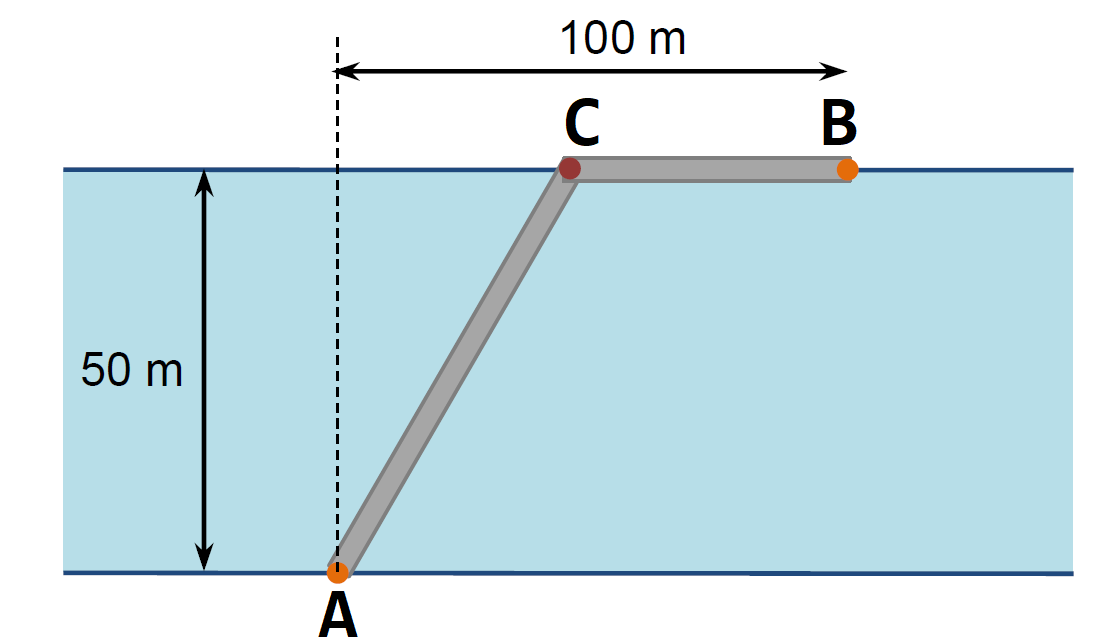
\includegraphics[width=0.45\textwidth]{figures/Behaviour/fig_behaviour_33}}
\caption{Schematic representation of the pipeline from Exercise~\ref{oef_pijpleiding}.}
\label{fig_behaviour_33}

\end{figure}

\end{Exercise}

\begin{Answer}\phantom{}
    The minimum cost is achieved for a distance of 83.32 m between the point $B$ and the point $C$.
\end{Answer}

%%%%%%%%%%%%%%%%%
%Oefening 9 Ings
%%%%%%%%%%%%%%%

\begin{Exercise}[difficulty = 2, label = oef_lodenbuis] A lead pipe is transported horizontally through a corridor that is 3 m wide (Figure~\ref{fig_behaviour_34}). At the end of the corridor, there is a 90-degree turn and the corridor narrows to 2 m. What is the length of the largest tube that can be carried horizontally around the corner?

%Uit: Bocher H3 
\begin{figure}[H]
\centerline{
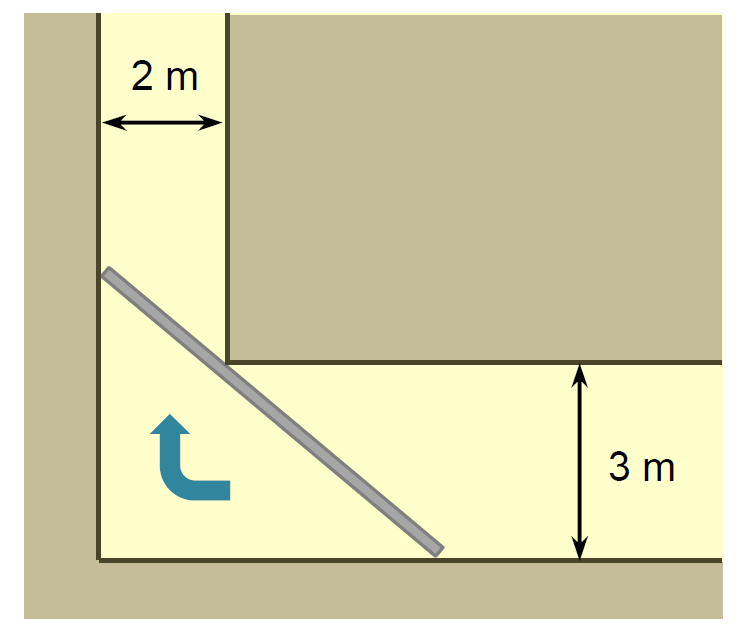
\includegraphics[width=0.35\textwidth]{figures/Behaviour/fig_behaviour_34}}
\caption{Schematic representation of the lead pipe from Exercise~\ref{oef_lodenbuis}.}
\label{fig_behaviour_34}
\end{figure}

\end{Exercise}

\begin{Answer}\phantom{}
    The length of the largest tube that can be carried horizontally around the corner is 7.02 m.
\end{Answer}

%%%%%%%%%%%%%%%%%
%Oefening 10 Ings
%%%%%%%%%%%%%%%
%Uit: Bocher H3 
\begin{Exercise}[difficulty = 2, label = oef_melkdoos] A cardboard box of capacity 0.5 l is formed from a piece of plasticized cardboard as shown in Figure~\ref{fig_behaviour_35}. The base is a square with side $B$, the dotted lines indicate the fold lines and the gray strips are for gluing. Determine the height $H$ and the base $B$ to obtain 0.5 l as a volume with a minimum amount of cardboard. 

\begin{figure}[H]
\centerline{
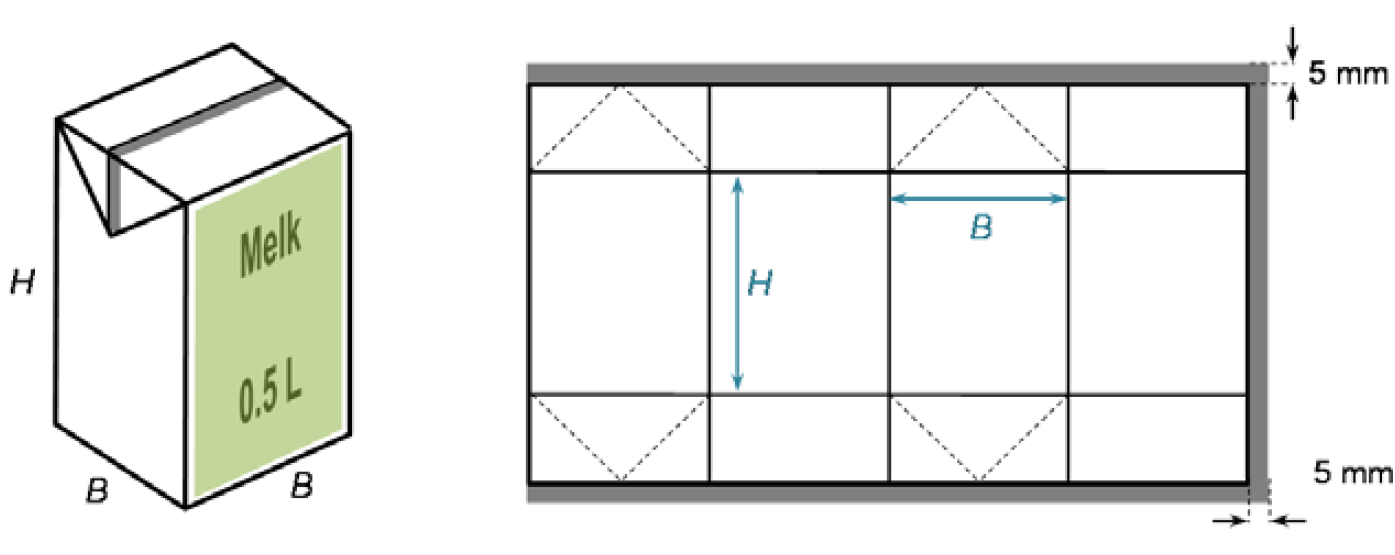
\includegraphics[width=0.75\textwidth]{figures/Behaviour/fig_behaviour_35}}
\caption{Schematic representation of the milk box from Exercise~\ref{oef_melkdoos}.}
\label{fig_behaviour_35}
\end{figure}

\end{Exercise}

\begin{Answer}\phantom{}
    A minimal amount of cardboard is consumed if $B=6.2$ cm and $H=13$ cm.
\end{Answer}

%%%%%%%%%%%%%%%%%
%Oefening 11 Ings
%%%%%%%%%%%%%%%
%Uit: Bocher H3 
\begin{Exercise}[difficulty = 3] A conical solid of revolution lies completely inside a sphere of radius $R$ cm. The top of the cone lies on the sphere and its axis is a diameter of the sphere. The volume of a cone is given by
$$
V=\dfrac{\pi r^2h}{3}\,,
$$
where $r$ is the radius of the base and $h$ is the height of the cone.

Calculate $r$ and $h$ such that the volume of the cone is maximal. 

\end{Exercise}

\begin{Answer}\phantom{}
    The volume of the cone is maximal for $h=4/3R$ and $r=2\sqrt{2}/3R$.
\end{Answer}
\fi


\subsection*{Review exercises}
%%%%%%%%%%%%%%%%%
%Oefening 1
%%%%%%%%%%%%%%%%%
\begin{Exercise}[difficulty = 2, label = oef_functie_afgeleiden] Figure \ref{fig_behaviour_31} shows the graph of a function $f$, its derivative functions $f'$ and $f''$ and a function $g$. Which graph corresponds to which function? 
\begin{figure}[H]
\centerline{
\subfigure[]{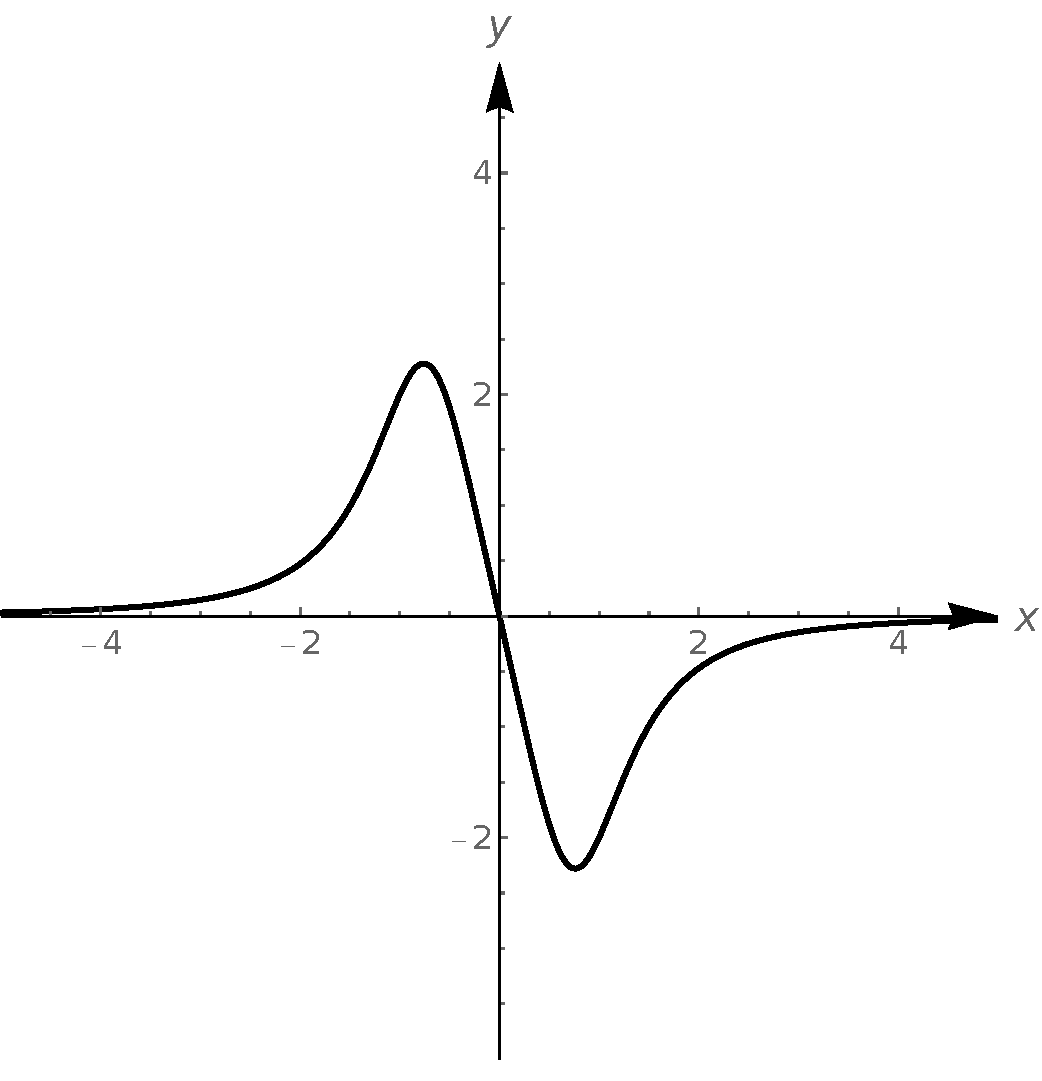
\includegraphics[width=0.25\textwidth]{fig_behaviour_31a}}
\hspace{0.1cm}
\subfigure[]{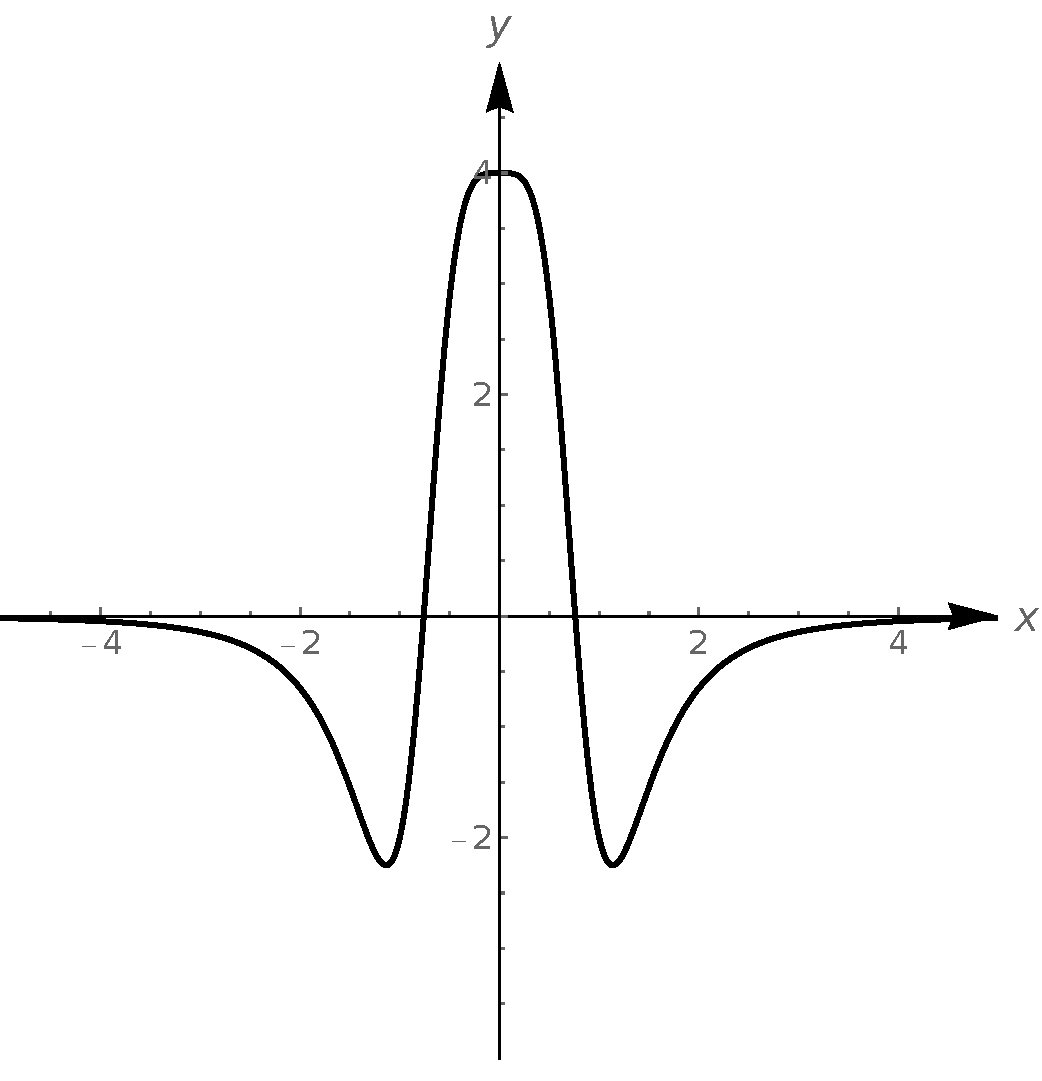
\includegraphics[width=0.25\textwidth]{fig_behaviour_31b}}}
\centerline{
\subfigure[]{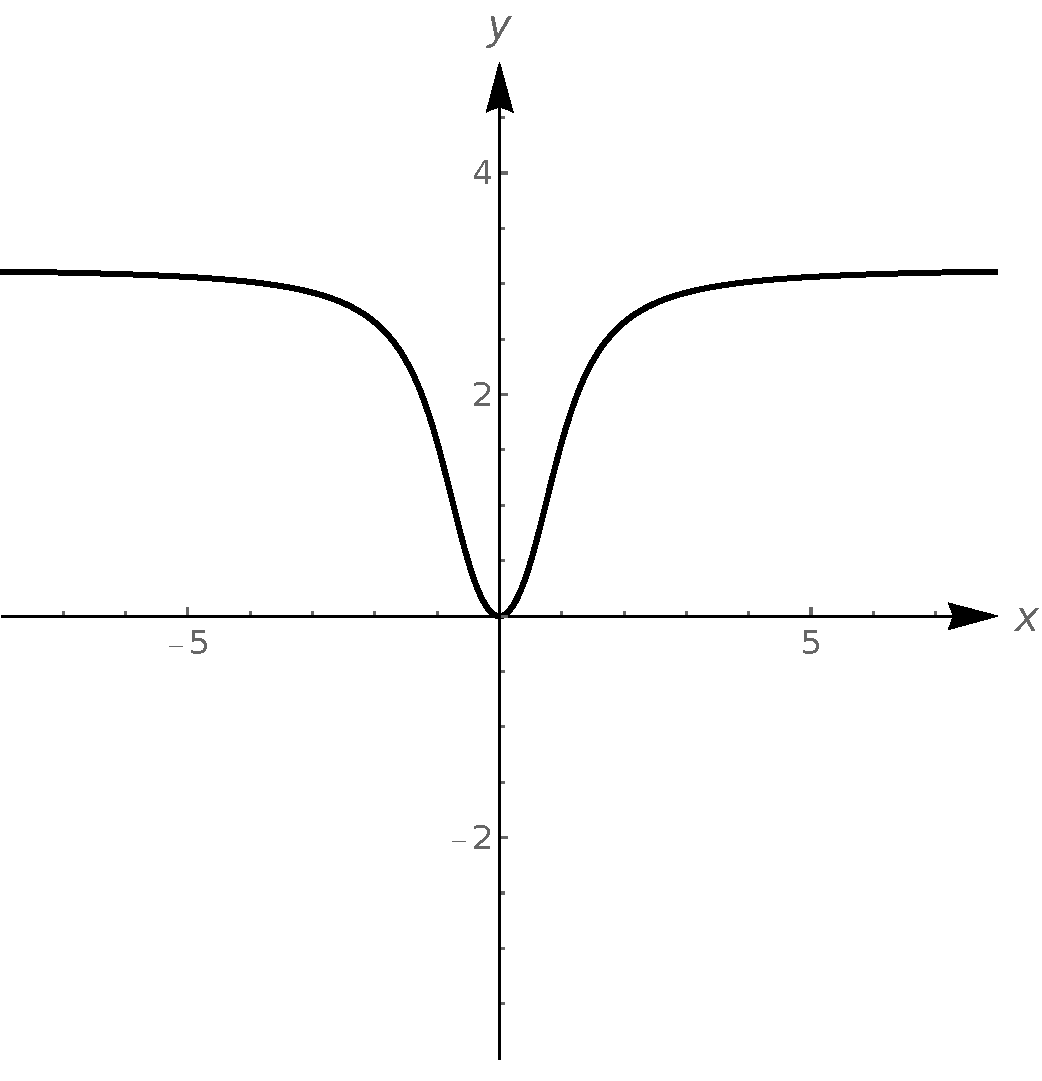
\includegraphics[width=0.25\textwidth]{fig_behaviour_31c}}
\hspace{0.1cm}
\subfigure[]{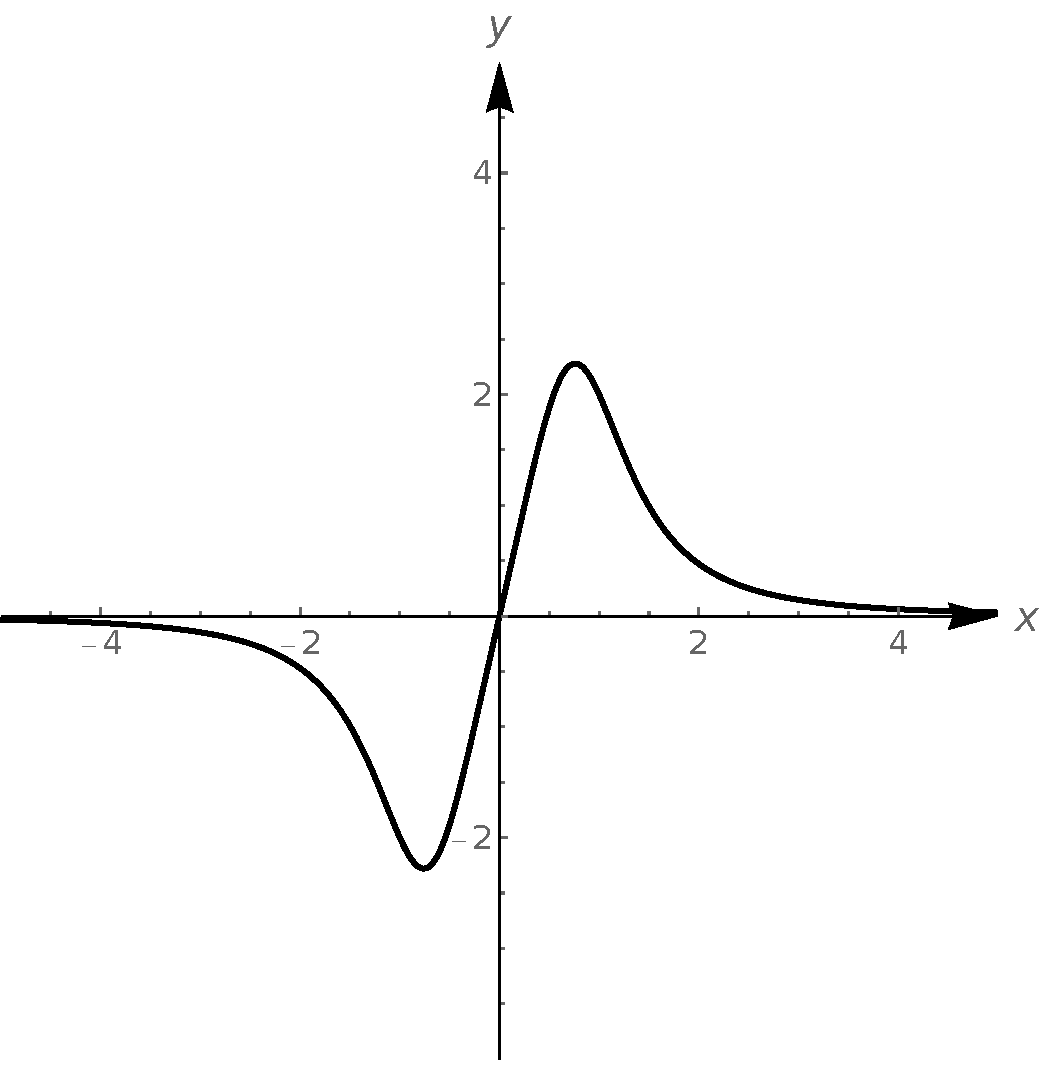
\includegraphics[width=0.25\textwidth]{fig_behaviour_31d}}
}
\caption{Figure belonging to Exercise~\ref{oef_functie_afgeleiden}}
\label{fig_behaviour_31}
\end{figure}
\end{Exercise}

%\setboolean{firstanswerofthechapter}{true}
\begin{Answer}\phantom{}
    Graph (c) is the graph of $f$, (d) is the graph of $f'$, (b) is the graph of $f''$ and (a) is that of the function $g$.
\end{Answer}
%\setboolean{firstanswerofthechapter}{false}

%%%%%%%%%%%%%%%%%
%Oefening 2
%%%%%%%%%%%%%%%
\ifanalysis\begin{Exercise}[difficulty = 1, label = oef_functieverloop]\fi \ifcalculus\begin{Exercise}[difficulty = 2, label = oef_functieverloop]\fi 
Figure \ref{fig_behaviour_32} shows the graphs of four functions:
\[ f(x) = \dfrac{x}{1-x^2}, \qquad g(x) = \dfrac{x^3}{1-x^4}, \qquad h(x) = \dfrac{x^3 - x}{\sqrt{x^6+1}} \qquad \text{ and } \qquad k(x) = \dfrac{x^3}{\sqrt{|x^4-1|}}.\]

Which graph corresponds to which function?
\begin{figure}[H]
\centerline{
\subfigure[]{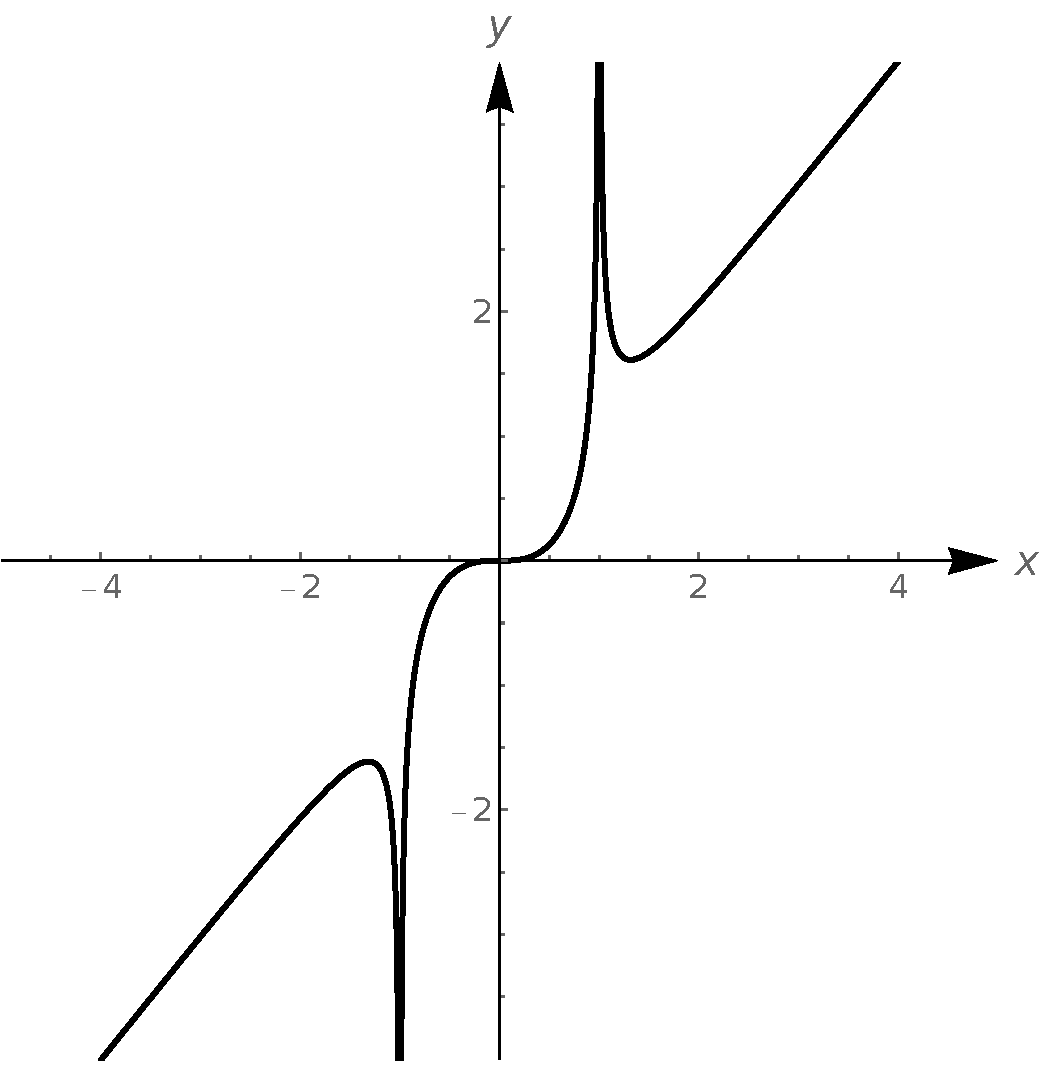
\includegraphics[width=0.25\textwidth]{figures/Behaviour/fig_behaviour_32a}}
\hspace{0.1cm}
\subfigure[]{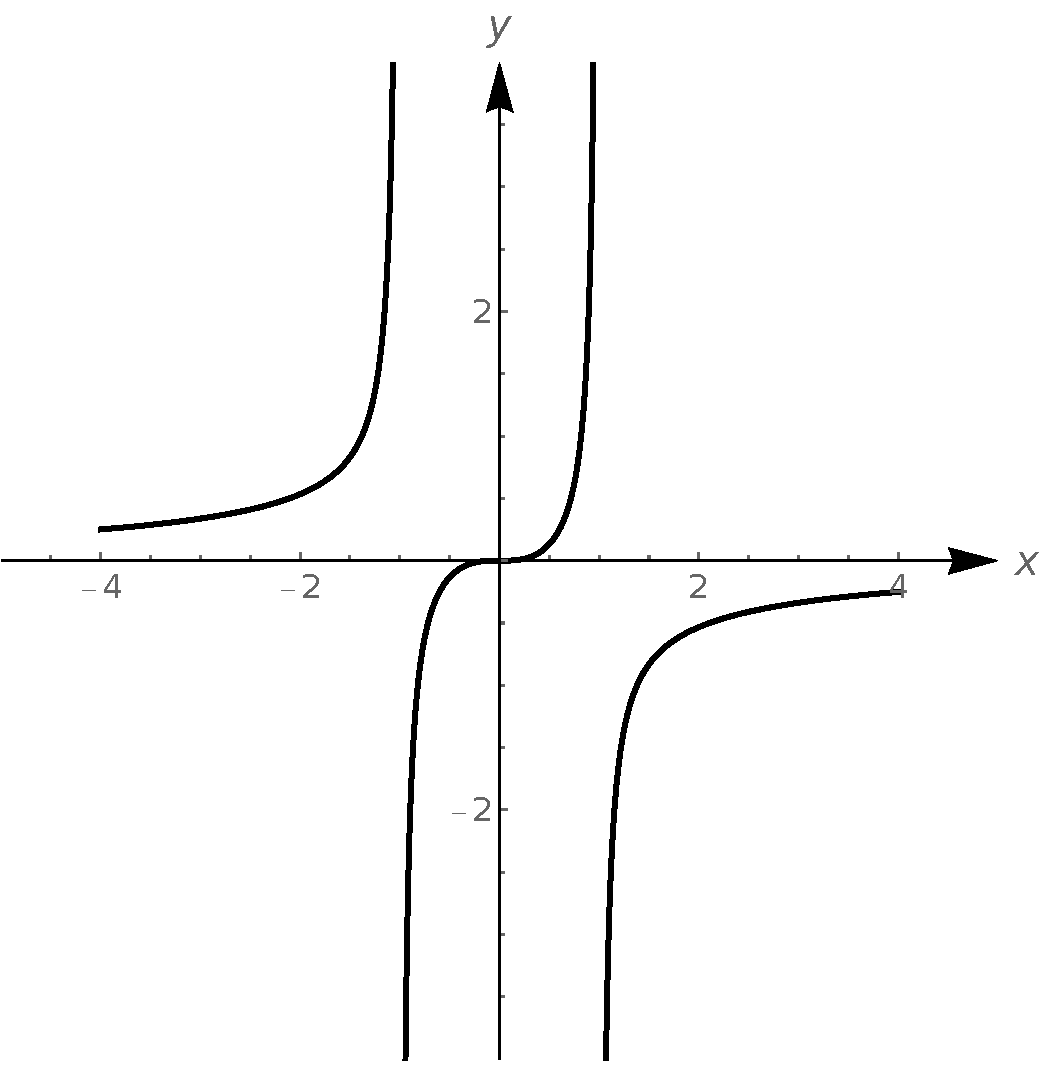
\includegraphics[width=0.25\textwidth]{figures/Behaviour/fig_behaviour_32b}}}
\centerline{
\subfigure[]{\includegraphics[width=0.25\textwidth]{figures/Behaviour/fig_behaviour_32c}}
\hspace{0.1cm}
\subfigure[]{\includegraphics[width=0.25\textwidth]{figures/Behaviour/fig_behaviour_32d}}
}
\caption{Figure corresponding to exercise~\ref{oef_functieverloop}.}
\label{fig_behaviour_32}

\end{figure}

\ifanalysis\end{Exercise}\fi\ifcalculus\end{Exercise}\fi

\begin{Answer}\phantom{}
    Graph (c) is the graph of $f(x) = \dfrac{x}{1-x^2}$, graph (b) is the graph of $g(x) = \dfrac{x^3}{1-x^4}$, graph (d) is the graph of $h(x) = \dfrac{x^3 - x}{\sqrt{1+x^6}}$ graph (a) is the graph of $k(x) = \dfrac{x^3}{\sqrt{|x^4-1|}}$.
\end{Answer}


%%%%%%%%%%%%%%%%%
%Oefening 5
%%%%%%%%%%%%%%%
\begin{Exercise} For the functions below, if possible, determine the local maxima and/or minima and any inflection points. Also determine the intervals where the function is convex or concave.
\begin{multicols}{2}
    \Question[difficulty = 1] $f(x) = 2x^3-3x^2+9x+5 $
    \ifcalculus\Question[difficulty = 1] $f(x) = (x-1)^2(x+2) $\fi
    \ifanalysis\Question[difficulty = 1]\fi\ifcalculus\Question[difficulty = 2]\fi $f(x) = \dfrac{1}{x^2+1}$
    \Question[difficulty = 1] $f(x) = \sin (x) + \cos (x), \qquad x \in ]-\pi,\pi[$ 
    \Question[difficulty = 1] $f(x) = x^2 \ln (x) $ 
    \EndCurrentQuestion
\end{multicols}

\end{Exercise}

\begin{Answer}\phantom{}
    
        \Question 
            \begin{itemize}
                \item local maxima/minima: none,
                \item infliction points: $x=1/2$,
                \item concave over $]-\infty, 1/2[$, convex over $] 1/2, +\infty[$.
             \end{itemize}
             \ifcalculus
        \Question 
            \begin{itemize}
                \item local maxima/minima: local max. in $(-1,4)$, local min. in $(1,0)$,
                \item infliction points: $x=0$,
                \item concave over $]-\infty, 0[$, convex over $] 0, +\infty[$.
             \end{itemize}
             \fi
        \Question 
           \begin{itemize}
                \item local maxima/minima: global max. in $(0,1)$,
                \item infliction points: $x=\pm \sqrt{3}/3$,
                \item concave over $]-\sqrt{3}/3, \sqrt{3}/3[$, convex over $]-\infty, -\sqrt{3}/3[ \cup ]\sqrt{3}/3, +\infty[$.
             \end{itemize}
             
        \Question 
            \begin{itemize}
                \item local maxima/minima: global max. in $(\pi/4,\sqrt{2})$, global min. in $(-3\pi/4,-\sqrt{2})$,
                \item infliction points: $x=- \pi/4, 3\pi/4$,
                \item concave over $]- \pi/4, 3\pi/4[$, convex over $]-\pi, -\pi/4[ \cup ]3\pi/4, \pi[$.
            \end{itemize}
            
        \Question 
            \begin{itemize}
                \item local maxima/minima: global min. in $(e^{-1/2},-e/2)$,
                \item infliction points: $x=1/e^{3/2}$,
                \item concave over $]0, 1/e^{3/2}[$, convex over $]1/e^{3/2}, + \infty[$.
            \end{itemize}
   
\end{Answer}


\ifanalysis
%%%%%%%%%%%%%%%%%
%Oefening 7 Bio-irs
%%%%%%%%%%%%%%%
\begin{Exercise} Describe the critical points and possible inflection points of the function $f$ as a function of $a$ and $b$. 
\begin{multicols}{2}
	\Question[difficulty = 1] $f(x) = \dfrac{a}{x^2+b^2}$
	\Question[difficulty = 2] $f(x) = \sin (ax+b)$
    \EndCurrentQuestion
\end{multicols}

\end{Exercise}

\begin{Answer}\phantom{}
    
	\Question 
	Critical points: $x=0$  \\
	Infliction points: $x=\pm \sqrt{\dfrac{b^2}{3}}$
	\Question 
	Critical points: $x=\dfrac{n \pi/2-b}{a},$ with $n \in \mathbb{Z}$ odd \\
	Infliction points: $x=\dfrac{n \pi-b}{a},$ with $n \in \mathbb{Z}$
   
\end{Answer}

\fi